\documentclass[%
%%% PARA ESCOLHER O ESTILO TIRE O SIMBOLO %(COMENTÁRIO)
%SemVinculoColorido,
%SemFormatacaoCapitulo,
%SemFolhaAprovacao,
%SemImagens,
%CitacaoNumerica, %% o padrão é citação tipo autor-data
PublicacaoDissOuTese, %% (é também o "default") com ficha catal. e folha de aprovação em branco. Caso tenha lista de símbolos e lista de siglas e abreviaturas retirar os comentários dos arquivos siglas.tex e abreviaturasesiglas.tex. Retirar também os comentários indicados nesse arquivo, nos includes
%PublicacaoArtigoOuRelatorio, %% texto sequencial, sem quebra de páginas nem folhas em branco
%PublicacaoProposta, %% igual tese/dissertação, mas sem ficha catal. e fol. de aprov.
%PublicacaoLivro, %% com capítulos
%PublicacaoLivro,SemFormatacaoCapitulo, %% sem capítulos
%english,portuguese %% para os documentos em Português com abstract.tex em Inglês
portuguese,english %% para os documentos em Inglês com abstract.tex em Português
,LogoINPE% comentar essa linha para fazer aparecer o logo do Governo (Ex.: LogoINPE usado em ano eleitoral). Caso deseje alterar o logo governo verificar a pasta .template/logo/logoverno.png
,CCBYNC	% as opções de licença são: CCBY, CCBYSA, CCBYND, CCBYNC, CCBYNCSA, CCBYNCND, GPLv3 e INPECopyright
]{./template/tdiinpe}
%\documentclass[english,portuguese,LogoINPE,CCBYNC]{http://urlib.net/iconet.com.br/banon/2008/03.25.01.19/tdiinpe}

% PARA EXIBIR EM ARIAL TIRAR O COMENTÁRIO DAS DUAS LINHAS SEGUINTES
%\renewcommand{\rmdefault}{phv} % Arial
%\renewcommand{\sfdefault}{phv} % Arial

%%%%%%%%%%%%%%%%%%%%%%%%%%%%%%%%%%%%%%%%%%%%%
%%% Pacotes já previamente carregados:      %
%%%%%%%%%%%%%%%%%%%%%%%%%%%%%%%%%%%%%%%%%%%%%%%%%%%%%%%%%%%%%%%%%%%%%%%%
%%% ifthen,calc,graphicx,color,inputenc,babel,hyphenat,array,setspace, %
%%% bigdelim,multirow,supertabular,tabularx,longtable,lastpage,lscape, %
%%% rotate,caption2,amsmath,amssymb,amsthm,subfigure,tocloft,makeidx,  %
%%% eso-pic,calligra,hyperref,ae,fontenc                               %
%%%%%%%%%%%%%%%%%%%%%%%%%%%%%%%%%%%%%%%%%%%%%%%%%%%%%%%%%%%%%%%%%%%%%%%%
%%% insira neste campo, comandos de LaTeX %%%
%%% \usepackage{_exemplo_}
% etc.
%%%%%%%%%%%%%%%%%%%%%%%%%%%%%%%%%%%%%%%%%%%%%

%\watermark{Revisão No. ##} %% use o comando \watermark para identificar a versão de seu documento
%% comente este comando quando for gerar a versão final
\usepackage{rotating}
\usepackage{dsfont}
\usepackage{booktabs}
\usepackage{comment}
\usepackage{pdfpages}
\usepackage{makecell} 
\usepackage{longtable}
\usepackage{array}  % no preâmbulo


%%%%%%%%%%%%%%%%%%%CAPA%%%%%%%%%%%%%%%%%%%%%%%%%%%%%%%%
%\serieinpe{INPE-NNNNN-TDI/NNNN} %% não mais usado

\titulo{Exploring Cold Pool Dynamics in MONAN: Insights from Hurricanes}
\title{Explorando a Dinâmica de \textit{Cold Pools} no MONAN: Perspectivas a partir de Furacões} %% 
\author{Bianca Fusinato} %% coloque o nome do(s) autor(es)
\descriccao{Master's Dissertation from the Graduate Program in Meteorology, supervised by Dr. Saulo R. Freitas, approved on [day] of [month] [year].}
\repositorio{aa/bb/cc/dd} %% repositório onde está depositado este documento - na omissão, será preenchido pelo SID
\tipoDaPublicacao{TDI}	%% tipo da publicação (NTC, RPQ, PRP, MAN, PUD, TDI, TAE e PRE) na ausência do número de série INPE, caso contrário deixar vazio
\IBI{xx/yy} %% IBI (exemplo: J8LNKAN8PW/36CT2G2) quando existir, caso contrário o nome do repositório onde está depositado o documento

\date{2025}%ano da publicação

%%%%%%%%%%%%%%%%%%%%%%%%%%VERSO DA CAPA%%%%%%%%%%%%%%%%%%%%%%%%%%%%%%%%%%%%%%%%%%%%%%%
\tituloverso{\vspace{-0.9cm}\textbf{\PublicadoPor:}}
\descriccaoverso{Instituto Nacional de Pesquisas Espaciais - INPE\\
Coordenação de Ensino, Pesquisa e Extensão (COEPE)\\
Divisão de Biblioteca (DIBIB)\\
CEP 12.227-010\\
São José dos Campos - SP - Brasil\\
Tel.:(012) 3208-6923/7348\\
%Fax: (012) 3208-6919\\
E-mail: {pubtc@inpe.br}
}
\descriccaoversoA{\textbf{\ConselhoDeEditoracao:}\\
\textbf{\Presidente:}\\
Dra. Marley Cavalcante de Lima Moscati -  Coordenação-Geral de Ciências da Terra (CGCT)\\
\textbf{\Membros:}\\
Dra. Ieda Del Arco Sanches - Conselho de Pós-Graduação (CPG)\\
Dr. Evandro Marconi Rocco - Coordenação-Geral de Engenharia, Tecnologia e Ciência Espaciais  (CGCE)\\
Dr. Rafael Duarte Coelho dos Santos - Coordenação-Geral de Infraestrutura e Pesquisas Aplicadas (CGIP)\\
Simone Angélica Del Ducca Barbedo - Divisão de Biblioteca (DIBIB)\\
\textbf{\BibliotecaDigital:}\\
Dr. Gerald Jean Francis Banon \\
Clayton Martins Pereira - Divisão de Biblioteca (DIBIB)\\
%Jefferson Andrade Ancelmo - Divisão de Biblioteca (DIBIB)\\
%Simone A. Del-Ducca Barbedo - Divisão de Biblioteca (DIBIB)\\
%Deicy Farabello - Centro de Previsão de Tempo  e Estudos Climáticos (CGCPT)\\
\textbf{\RevisaoNormalizacaoDocumentaria:}\\
Simone Angélica Del Ducca Barbedo - Divisão de Biblioteca (DIBIB) \\
%Marilúcia Santos Melo Cid - Divisão de Biblioteca (SID)\\
%Yolanda Ribeiro da Silva Souza - Divisão de Biblioteca (DIBIB)\\
André Luis Dias Fernandes - Divisão de Biblioteca (DIBIB)\\
\textbf{\EditoracaoEletronica:}\\
Ivone Martins - Divisão de Biblioteca (DIBIB)\\
André Luis Dias Fernandes - Divisão de Biblioteca (DIBIB)\\
}

%%%%%%%%%%%%%%%%%%%FOLHA DE ROSTO

%%%%%%%%%%%%%%%FICHA CATALOGRÁFICA
%% NÃO PREENCHER - SERÁ PREENCHIDO PELO SID

\cutterFICHAC{Cutter}
\autorUltimoNomeFICHAC{Sobrenome, Nomes} %% exemplo: Fuckner, Marcus André
\autorFICHAC {Nome Completo do Autor1; Nome Completo do Autor2} %% Campo opcional (se não usado prevalece \author)
\tituloFICHAC{Titulo da publicação}
\instituicaosigla{INPE}
\instituicaocidade{São José dos Campos}
\paginasFICHAC{\pageref{numeroDePáginasDoPretexto} + \pageref{LastPage}} %% número total de páginas
%\serieinpe{INPE-00000-TDI/0000} %% não mais usado
\palavraschaveFICHAC{1.~Palavra chave. 2.~Palavra chave 3.~Palavra chave. 4.~Palavra chave. 5.~Palavra chave  I.~\mbox{Título}.} %% recomenda-se pelo menos 5 palavras-chaves - \mbox{} é para evitar hifenização 
\numeroCDUFICHAC{000.000} %% número do CDU 

% Nota da ficha (para TD)
\tipoTD{Dissertação ou Tese} % Dissertação ou Tese
\cursoFA{Mestrado ou Doutorado em Nome do Curso}
\instituicaoDefesa{Instituto Nacional de Pesquisas Espaciais}
\anoDefesa{AAAA} % ano de defesa 
\nomeAtributoOrientadorFICHAC{Orientador}	% pode ser: Orientador, Orientadora ou Orientadores
\valorAtributoOrientadorFICHAC{José da Silva} % nome(s) completo(s)

%%%%%%%%%%%%%%%FOLHA DE APROVAÇAO PELA BANCA EXAMINADORA
\tituloFA{\textbf{ATENÇÃO! A FOLHA DE APROVAÇÃO SERÁ INCLUIDA POSTERIORMENTE.}}
%\cursoFA{\textbf{}}
\candidatoOUcandidataFA{}
\dataAprovacaoFA{}
\membroA{}{}{}
\membroB{}{}{}
\membroC{}{}{}
\membroD{}{}{}
\membroE{}{}{}
\membroF{}{}{}
\membroG{}{}{}
\ifpdf

%%%%%%%%%%%%%%NÍVEL DE COMPRESSÃO {0 -- 9}
\pdfcompresslevel 9
\fi
%%% define em 80% a largura das figuras %%%
\newlength{\mylenfig} 
\setlength{\mylenfig}{0.8\textwidth}
%%%%%%%%%%%%%%%%%%%%%%%%%%%%%%%%%%%%%%%%%%%

%%%%%%%%%%%%%%COMANDOS PESSOAIS
\newcommand{\vetor}[1]{\mathit{\mathbf{#1}}} %% faça as modificações pertinentes no arquivo configuracao.tex

\makeindex  %% não alterar, gera INDEX, caso haja algum termo indexado no texto

\begin{document} %% início do documento %% não mexer

%\marcaRegistrada{}	% comando opcional usado para informar abaixo da ficha catalográfica sobre marca registrada
\marcaRegistrada{Informar aqui sobre marca registrada (a modificação desta linha deve ser feita no arquivo publicacao.tex).}
%\financiamento{}	% comando opcional usado para informar abaixo da ficha catalográfica sobre fontes financiadoras
\financiamento{Informar aqui sobre fontes financiadoras (a modificação desta linha deve ser feita no arquivo publicacao.tex).}
%\financiamento{O presente trabalho foi realizado com apoio da Coordenação de Aperfeiçoamento de Pessoal de Nível Superior - Brasil (CAPES) - Código de Financiamento 001.}
%\financiamento{This study was financed in part by the Coordenação de Aperfeiçoamento de Pessoal de Nível Superior - Brasil (CAPES) - Finance Code 001.}

\maketitle  %% não alterar, gera páginas obrigatórias (folha de rosto, ficha catalográfica e folha de aprovação), automaticamente

%%% Comente as linhas opcionais abaixo caso não as deseje
%%%%%%%%%%%%%%%%%%%%%%%%%%%%%%%%%%%%%%%%%%%%%%%%%%%%%%%%%%%%%%%%%%%%%%%%%%%%%%%%%
% Epígrafe %% opcional

\begin{epigrafe} %% insira sua epígrafe abaixo; estilo livre

%\hypertarget{estilo:epigrafe}{} %% uso para este Guia
 
\textit{\large``A vida será mais complicada se você possuir uma curiosidade ativa, além de aumentarem as chances de você entrar em apuros, mas será mais divertida''.}

\vspace{1cm}

\hspace{4cm} \emph{\textsc{Edward Speyer}} \hspace{4cm} em \textsl{``Seis Caminhos a Partir de Newton''}, 1994

\end{epigrafe} %% Opcional
%%%%%%%%%%%%%%%%%%%%%%%%%%%%%%%%%%%%%%%%%%%%%%%%%%%%%%%%%%%%%%%%%%%%%%%%%%%%%%%%%
% Dedicatória %% opcional

\begin{dedicatoria} %% insira sua dedicatória abaixo; estilo livre

%\hypertarget{estilo:dedicatoria}{} %% uso para este Guia
 
%% use 'a meus' em vez de 'aos meus', isto é, não use o artigo definido com pronomes possessivos

\newcommand{\mytext}{A meus pais \textbf{Nicanor} e \textbf{Jaci}, à minha irmã \textbf{Luciana} e ao meu esposo \textbf{William}}

\begin{comment}
%%% sugestão de estilo
\ifcalligra %% fonte calligra presente nas versões mais novas do MiKTeX (>= 2.4)
  \calligra\Large \mytext %% exemplo usando estilo de fonte caligráfica, caso haja
\else
	\itshape\Large \mytext 
\fi
\end{comment}

	\itshape\Large \mytext 

\end{dedicatoria} %% Opcional
%%%%%%%%%%%%%%%%%%%%%%%%%%%%%%%%%%%%%%%%%%%%%%%%%%%%%%%%%%%%%%%%%%%%%%%%%%%%%%%%
% AGRADECIMENTOS %% opcional

\begin{agradecimentos}  %% insira abaixo seus agradecimentos

%\hypertarget{estilo:agradecimentos}{} %% uso para este Guia

acknowledges 

\end{agradecimentos}


 %% Opcional
%%%%%%%%%%%%%%%%%%%%%%%%%%%%%%%%%%%%%%%%%%%%%%%%%%%%%%%%%%%%%%%%%%%%%%%%%%%%%%%%
% RESUMO %% obrigatório

\begin{resumo}

%% neste arquivo resumo.tex
%% o texto do resumo e as palavras-chave têm que ser em Português para os documentos escritos em Português
%% o texto do resumo e as palavras-chave têm que ser em Inglês para os documentos escritos em Inglês
%% os nomes dos comandos \begin{resumo}, \end{resumo}, \palavraschave e \palavrachave não devem ser alterados

%\hypertarget{estilo:resumo}{} %% uso para este Guia

Structure:
GCMs and the need of parameterization, including sub-grid phenomena

Explain about the cold pools and the parameterization

Explain the dissertation’s goal: explore this cold pool parameterization and select the best bulk of features to configure the CPTEC model

How are we going to do it? 

Since we are working with hurricanes propagating in the ocean, we test other parameterization to take into account - How does it work?

Leave a paragraph to insert the results.


Inside Global Circulation Models (GCMs), precipitation can be modeled through cloud microphysics or convection schemes. Despite advancements in computational capabilities, computational constraints still imply the need for parameterizations for processes not explicitly resolved at the model's grid-scale.%, especially in Earth System or climate models. 


% I need to changes this
It has been shown that to improve large-scale numerical representation it can be started by improving the sub-grid scale process representation. %For example, a significant way to generate the propagating convection on squall lines, essential for the Amazon rain patterns, is through cold pools, which is the subject matter of this proposal.



Cold Pools correspond to a cold air mass descending within the downdraft. Recent studies show that cold pools are divided into two structures: the cold and dry centers and a moist ring on the edge. When it reaches the surface, it spreads out horizontally, and the high values of moist static energy on the rings combined with the gust front speed can lift the air thermodynamically and mechanically, respectively. 

The spatial scale of this phenomenon is translated into sub-grid numerical representations inside the GCMs. It has been shown that cold pools can organize the formation of new convective cells, promoting their aggregation and leading to the development of mesoscale convective systems.  

An investigation of the impact of the cold pool parameterization using simulations performed with the Model for Ocean-LaNd-Atmosphere PredictionN (MONAN) is proposed. %The experiments are composed by the 2024 Hurricane Beryl, from June 28 to July 13; and three periods in 2014 over the Amazon Rainforest, each lasting 10 days: the wet season (15–24 FEB), the dry season (01–10 SEP), and the transition from dry to wet (01–10 OCT). Alongside this, an investigation of the performance of the cold pool parameterization during sensitivity test inside the hurricane and over the Amazon diurnal cycle of precipitation aimed to be accomplished. Finally, to quantify the effect of cold pool parameterization on convective organization, the $L_{\text{org}}$ index will be employed. All the results were compared with GPM-IMERG precipitation data and ERA5 data.

% Não fica claro a importância medição da organização convectiva induzida por cold pools.

\palavraschave{%
	\palavrachave{GCM}%
        \palavrachave{Cold Pool}%
	\palavrachave{MONAN}%
	\palavrachave{Hurricanes}%
	\palavrachave{Sea Spray}%
}
 
\end{resumo} %% obrigatório
%%%%%%%%%%%%%%%%%%%%%%%%%%%%%%%%%%%%%%%%%%%%%%%%%%%%%%%%%%%%%%%%%%%%%%%%%%%%%%%%
% ABSTRACT

\begin{abstract}

%% neste arquivo abstract.tex
%% o texto do resumo e as palavras-chave têm que ser em Inglês para os documentos escritos em Português
%% o texto do resumo e as palavras-chave têm que ser em Português para os documentos escritos em Inglês
%% os nomes dos comandos \begin{abstract}, \end{abstract}, \keywords e \palavrachave não devem ser alterados

\selectlanguage{portuguese}	%% para os documentos escritos em Português
%\selectlanguage{portuguese}	%% para os documentos escritos em Inglês

%\hypertarget{estilo:abstract}{} %% uso para este Guia

Traduzir o resumo para português

\keywords{%
	\palavrachave{}%
	\palavrachave{}%
	\palavrachave{}%
	\palavrachave{}%
	\palavrachave{}%
}

\selectlanguage{portuguese}	%% para os documentos escritos em Português
%\selectlanguage{english}	%% para os documentos escritos em Inglês

\end{abstract} %% obrigatório

\includeListaFiguras %% obrigatório caso haja mais de 3 figuras, gerado automaticamente
\includeListaTabelas %% obrigatório caso haja mais de 3 tabelas, gerado automaticamente

%%%%%%%%%%%%%%%%%%%%%%%%%%%%%%%%%%%%%%%%%%%%%%%%%%%%%%%%%%%%%%%%%%%%%%%%%%%%%%%%
%abreviaturas e siglas  %% opcional, mas recomendado

\begin{abreviaturasesiglas}  %% insira abaixo suas abreviaturas conforme o modelo.

%% sigla (separador: &--&) significado (quebra de linha: \\)
%\\

% WETAMC   &--&   Campanha de Mesoescala Atmosférica na Estação Úmida \\
% IBGE   &--& Instituto Brasileiro de Geografia e Estatística\\
% MC    &--&  Método das Covariâncias\\
% EDO   &--&  Equações Diferenciais Ordinárias\\
% EDP   &--&  Equações Diferenciais Parciais\\
% ECT   &--&  Energia Cinética Turbulenta\\
% FDP   &--&  Função de Distribuição de Probabilidade\\
% PR    &--&  Plot de Recorrência\\
% FFT   &--&  Fast Fourier Transform \\
% tS1200  &--&  Temperatura medida no nível superior às 12 horas \\
% tS2300  &--&  Temperatura medida no nível superior às 23 horas \\
% tM1200  &--&  Temperatura medida no nível médio às 12 horas \\
% tM2300  &--&  Temperatura medida no nível médio às 23 horas \\
% tI1200  &--&  Temperatura medida no nível inferior às 12 horas \\
% tI2300  &--&  Temperatura medida no nível inferior às 23 horas \\

\end{abreviaturasesiglas}
 %% opcional %% altere o arquivo siglaseabreviaturas.tex

%%%%%%%%%%%%%%%%%%%%%%%%%%%%%%%%%%%%%%%%%%%%%%%%%%%%%%%%%%%%%%%%%%%%%%%%%%%%%%%%
% simbolos

\begin{simbolos}

%% o comando: \hypertarget{estilo:simbolos}{} abaixo é de uso para este Guia
%% e pode ser retirado

\hypertarget{estilo:simbolos}{}

% a   &--& primeira contante \\
% b   &--& segunda constante \\
% $\rho$  &--& densidade de um fluido\\
% $\nu$   &--& viscosidade cinemática\\
% $R_{e}$  &--& número de Reynolds\\
% $\alpha$  &--& constante de Kolmogorov\\
% $k$ &--&  número de onda\\
% $K$ &--&  curtose\\
% $D_{0}$ &--& dimensão de contagem de caixas\\
% $D_{1}$ &--& dimensão de informação\\
% $D_{2}$  &--& dimensão de correlação\\
% $\lambda_{1}$  &--& expoente de Lyapunov dominante\\
 

\end{simbolos}

 %% opcional %% altere o arquivo simbolos.tex

\includeSumario  %% obrigatório, gerado automaticamente

\inicioIntroducao %% não altere este comando

%%%%%%%%%%%%%%%%%%%%%%%%%%%%%%%%%%%%%%%%%%%%%%%%%%%%%%%%%%%%%%%%%%%%%%%%%%%%%%%

\chapter{INTRODUCTION}

% Background and Context
% Reserach Problem
% Significance of Study

\section{General objective}

To explore a cold pool parameterization coupled with the Grell-Freitas convection parameterization within the Model for Ocean-laNd-Atmosphere predictioN (MONAN).


\section{Specific objectives}

\begin{enumerate}
    \item Assess the impact of the cold pool parameterization scheme on hurricane forecasted trajectory, intensity and rainfall;
    \item Perform sensitivity experiments within a hurricane case study, investigating the influence of initial conditions, cold pool duration, the displacement of the maximum mass flux height, type of initial condition and resolution;
    \item Identify the optimal parameter configuration for the cold pool parameterization to be used in MONAN;
    \item Evaluate the performance of this optimal configuration in other hurricane case study.
\end{enumerate}

\section{Scientific questions}

This work builds upon the findings and open issues identified in \citeonline{freitas2024parameterization}. The following scientific questions are proposed:

\begin{itemize}
    \item Does the GF-Cold Pool (GF-CP) scheme improve the forecast of hurricane trajectory, intensity, and rainfall in MONAN?
    \item Which parameters within the GF-CP have the most significant influence on hurricane representation in MONAN?
    \item How robust is the optimal GF-CP configuration when applied to a different hurricane event?
    \item Can improvements in cold pool representation lead to better rainfall predictions in tropical cyclones?
\end{itemize}
%% Think maybe in other two scientifics questions

\section{Thesis organization}

% This thesis is structured into seven chapters. Chapter 1 introduces the research, presenting its background, general and specific objectives, guiding scientific questions, and the overall structure of the work. Chapter 2 provides a review of the relevant literature, including the theoretical foundations of convective cloud dynamics, the mass-flux parameterization, cold pools, and the modeling of hurricanes. Chapter 3 describes the observational datasets and outlines the MONAN model configuration used throughout the study. Chapter 4 details the methodology, focusing on the diagnostic metrics and the workflow adopted to evaluate the cold pool parameterization scheme and its impact on hurricane forecasts. Chapter 5 presents a detailed case study of Hurricane Beryl, including a series of sensitivity experiments that lead to the identification of an optimal parameter configuration for the cold pool scheme. Chapter 6 applies this optimal setup to a second case, Hurricane Helene, in order to assess the robustness and generalization of the proposed configuration. Finally, Chapter 7 summarizes the main findings, addresses the initial scientific questions, discusses the scientific contributions and limitations of the work, and outlines recommendations for future research.




 %% 1o capítulo, começo do texto
%%%%%%%%%%%%%%%%%%%%%%%%%%%%%%%%%%%%%%%%%%%%%%%%%%%%%%%%%%%%%%%%%%%%%%%%%%%%%%%

\chapter{LITERATURE REVIEW}
\label{ch:convection}

% Theoretical Framework
% Current State of Knowledge
% Research Gaps
% Key Concepts and Definitions


%General aspects for understanding the Cold Pool (CP) phenomenon and its modeling aspects are presented in this chapter. Starting with the general convective structure, we provide a glimpse of atmospheric convection to characterize better the main features involved with CPs. The development of CPs and interaction features are explained next, focusing on Cloud Resolving Models (CRMs) and observational information. These features are crucial for understanding how CPs can trigger and organize new convection, subsequently upscaling them into Mesoscale Convective Systems (MCSs). Further on, a brief review of the Mass-Flux approach and the CP parameterization is outlined. Some aspects of the CP interacting with the selected study cases are described, to elucidate CP interacting with Hurricanes and their presence over the Amazon Basin. Finally, we conclude with the chosen convective organization metric.

\section{Overview of convective cloud dynamics}

\section{Cold pools}

\section{The mass-flux approach}

\section{The cold pool parameterization}

\section{Hurricanes - a model forecast view}

\section{Key points recall}




 %% 2o capítulo
\chapter{DATA AND MODEL}
\label{ch:data}

\section{Data}

This section presents the observational datasets used as a reference for evaluating the model forecasts. The selected datasets, described in detail in Sections \ref{section311} to \ref{section315}, are commonly employed in tropical cyclone studies and provide reliable information on storm trajectory, intensity, and precipitation. They have been used in several studies \cite{zhou2021regionalization, bopape2021sensitivity, dulac2024assessing, yang2024evaluation, may2024cnn} and support a robust assessment of the model's performance

\subsection{IBTrACS}
\label{section311}

The International Best Track Archive for Climate Stewardship (IBTrACS) \cite{knapp2010international} offers comprehensive data on the location and intensity of global tropical cyclones. It emphasizes parameters such as geographic position (latitude and longitude), maximum sustained wind speed (measured in knots), and minimum central pressure (in millibars). A complete list of variables and their definitions can be found at the provided link \footnote{\url{https://www.ncei.noaa.gov/sites/g/files/anmtlf171/files/2025-04/IBTrACS_version4r01_Technical_Details.pdf}}.

This dataset features a spatial resolution of 0.1° (approximately 10 km) and primarily reports data at a temporal resolution of 6 hours, although it can be interpolated to intervals of 3 hours; for our purposes, we will be utilizing the 6-hour data. The dataset covers the period from 1841 to the present, allowing users to explore it by searching for specific oceanic basins, including the North Atlantic, South Atlantic, Eastern North Pacific, Western North Pacific, South Pacific, South Indian, and North Indian.

The dataset is built upon information from various agencies. According to the documentation, the sources of this information include all available resources utilized by forecasters, such as surface observations, aircraft reconnaissance flights, and satellite observations.

\subsection{ERA5}

ERA5 \cite{hersbach2020era5} represents the fifth generation of atmospheric reanalysis conducted by the European Centre for Medium-Range Weather Forecasts (ECMWF), serving as a vital resource for both global climate and weather studies. This reanalysis integrates a forecast model with an advanced data assimilation scheme. Specifically, ERA5 employs the ECMWF Integrated Forecast System (IFS) CY41R2 forecast model, executing twice-daily short-term forecasts (18 hours) derived from analyses conducted at 06:00 and 18 UTC. Check the link \footnote{\url{https://www.ecmwf.int/en/elibrary/79697-ifs-documentation-cy41r2-part-iv-physical-processes}}
for a comprehensive understanding of the physical parameters encompassed within the model. The 4D-Var data assimilation method assimilates a diverse array of observations, including satellite data, ground station measurements, instrumented buoy data, and reconnaissance aircraft information. This process utilizes 12-hour time windows from 09 UTC to 21 UTC and from 21 UTC to 09 UTC (the subsequent day).

The initial configuration of the product involves 137 hybrid sigma/pressure levels in the vertical, with the uppermost level being at 0.01 hPa, and it maintains a horizontal resolution of 0.28125° (approximately 30km). Atmospheric data are accessible across interpolated 37 pressure levels. Consequently, the dataset comprises four primary subsets for download: hourly and monthly products, available on pressure levels (restricted to 37 levels) and single levels that encompass atmospheric, ocean-wave, and land surface quantities.

Reanalyses are not constrained by the necessity for timely forecasts, which allows for an extended period to collect observations. Furthermore, when assessing historical data, enhanced versions of the original observations can be integrated, thereby enhancing the quality of the reanalysis product. As a result, reanalyses provide a physically and dynamically consistent global representation of the atmospheric state at each time step. The major advantage of atmospheric reanalysis, particularly in the context of studying tropical cyclones, lies in its capacity to facilitate the analysis of the internal three-dimensional structure of contemporary TCs, alongside the large-scale environmental conditions surrounding them \cite{dulac2024assessing}.

The ERA5 data is accessible via the Climate Data Store and downloadable through the Climate Data Store (CDS) Application Program Interface (API). The variables under investigation are highlighted in the table below.



\begin{center}
	\captionof{table}{List of ERA5 Variables Used} \label{tab:era5_variables}
\end{center}

\begin{longtable}{p{3cm} p{8cm} p{2.5cm}}
	\toprule
	\textbf{Variable name} & \textbf{Long name} & \textbf{Unit} \\
	\midrule
	\endfirsthead
	
	\toprule
	\textbf{Variable name} & \textbf{Long name} & \textbf{Unit} \\
	\midrule
	\endhead
	
	\multicolumn{3}{r}{\textit{Table continued on next page}} \\
	\endfoot
	
	\bottomrule
	\endlastfoot
	
	msl *     & Mean sea level pressure                         & Pa \\
	i10fg *   & Instantaneous 10 metre wind gust                & m s\textsuperscript{-1} \\
	tp *      & Total precipitation                             & m \\
	sst *     & Sea Surface Temperature                          & K \\
	press **  & Pressure                                         & Pa \\
	u **      & U component of wind (Zonal Wind)                 & m s\textsuperscript{-1} \\
	v **      & V component of wind (Meridional Wind)            & m s\textsuperscript{-1} \\
	% Adicione mais linhas se necessário
\end{longtable}

\vspace{-1em}
\noindent\small Legend: * single levels; ** pressure levels.

\vspace{1em}
\begin{center}
	Source: Made by the author (2025).
\end{center}

\subsection{GPM-IMERG}

NASA’s Integrated Multi-satellite Retrievals for GPM (Global Precipitation Measurement) (IMERG) \cite{huffman2019gpm} algorithm synthesizes information from the GPM satellite constellation. Satellite data are particularly valuable to get information in areas of the Earth where ground-based precipitation-measuring instruments are limited, such as the Atlantic’s Main Development Region.

According to the Technical Documentation %\footnote{\url{https://arthurhou.pps.eosdis.nasa.gov/Documents/IMERG_TechnicalDocumentation_final.pdf}}
, estimates from various precipitation-relevant passive microwave (PMW) sensors within the GPM constellation are processed using an algorithm. These estimates are then gridded, intercalibrated with the GPM Combined Radar Radiometer Analysis product, and integrated into half-hourly fields with a horizontal resolution of 0.1° × 0.1°, covering latitudes from 60°S to 60°N. This data is provided to the Climate Prediction Center (CPC) Morphing-Kalman Filter (CMORPH-KF) quasi-Lagrangian time interpolation procedure, as well as undergoing a re-calibration that applies to the Precipitation Estimation from Remotely Sensed Information using Artificial Neural Networks (PERSIANN) Dynamic Infrared–Rain Rate (PDIR) infrared precipitation retrievals.

The product is offered in three stages: Early Run, Late Run, and Final Run. Researchers are encouraged to utilize the Final Run data for comprehensive analyses, as this stage incorporates monthly gauge data to create research-level products. However, it is important to note that the Final Run data has a latency period of approximately 3.5 months from the time of observation. Accordingly, we will employ the Final Run product, specifically using the NASA Goddard Earth Sciences (GES) Data and Information Services Center (DISC) V07 data, accessible through the link 
\footnote{\url{https://gpm.nasa.gov/data/directory}}
, last accessed on 16 May 2025, which offers precipitation data in netCDF format.

Lastly, concerning temporal distribution, this dataset, which covers the period from June 2000 to September 2021, is available for download every half-hour, daily, or monthly. For our analysis, we intend to concatenate the data to create hourly aggregates from the half-hourly product, which will subsequently be extrapolated to a resolution of approximately 30 km (our forecast resolution).


\subsection{GPM-MERGIR}

In the context of convective cloud modeling, it is essential to evaluate the model's capability to accurately represent cloud morphology. This assessment can be achieved through the analysis of infrared (IR) brightness temperature (Tb), also known as equivalent blackbody temperature, using satellite data. The observational dataset we are currently employing comes from the NASA GES DISC GPM Merged 4-Km IR Tb data set (GPM-MERGIR) \cite{janowiak2017ncep}, which is sourced from the NOAA Climate Prediction Center (CPC)/NCEP/NWS. The satellites contributing to this dataset include the Geosynchronous Operational Environmental Satellites (GOES) from the United States, the Geosynchronous Meteorological Satellite (GMS), followed by the Multi-functional Transport Satellite (MTSat) and Himawari from Japan, as well as the Meteorological Satellite (Meteosat) from the European Community, which forwards infrared (IR) imagery to the CPC. A complete list of these satellites can be found at this link %\footnote{\url{https://docserver.gesdisc.eosdis.nasa.gov/public/project/GPM/CPC-4kmIR-Sats.pdf}}.

The data is made available periodically in half-hour increments, covering latitudes from 60°S to 60°N with a pixel resolution of 4 km, dating back to 1 January 1998. In addition to direct downloads of netCDF-4 format data, GES DISC also provides data in binary, ASCII, and netCDF-3 formats via the OPeNDAP interface.

\subsection{GSMaP}
\label{section315}

Another satellite-based combined microwave-IR precipitation dataset will be utilized to evaluate precipitation generated by tropical cyclones. The Global Satellite Mapping of Precipitation (GSMaP), supported by the JAXA Precipitation Measuring Mission (PMM) Science Team, offers a multi-satellite global precipitation map as part of the Global Precipitation Measurement (GPM) Mission. It employs the Dual-frequency Precipitation Radar (DPR) onboard GPM core satellites, along with other GPM constellation satellites and geostationary satellites (website). Additionally, in the GSMaP products, apart from GSMaP\_NOW, the Globally-merged, full-resolution ($\sim$ 4km) infrared data produced by NOAA/CPC has also been utilized %\footnote{These details were obtained from the documentation available at \url{https://sharaku.eorc.jaxa.jp/GSMaP/guide.html\#01}.}.
The original data used for this product have been supplied by JAXA’s GSMaP.

The key feature of the GSMaP algorithm is its use of various attributes derived from the spaceborne precipitation radar, including TRMM/PR and GPM/DPR. This algorithm generates a rainfall rate product (in mm/hr) that covers a global extent (60°N to 60°S) with a horizontal resolution of 0.1° (latitude/longitude) and is available on an hourly basis.

The differences, features, and performance of this dataset compared to GPM-IMERG in tropical cyclone cases are widely discussed in the literature \cite{reddy2022accurately, bagtasa2022assessment, yang2024evaluation}.

\section{Numerical model: MONAN}

The model utilized for this study is part of the next generation of numerical models currently under development. The Model for Ocean-LaNd-Atmosphere Prediction (MONAN) is an advanced project by the Brazilian Centre of Weather and Climate Prediction (CPTEC) to become the new standard for weather and climate forecasting, nowcasting, and hindcasting. MONAN is an adaptation of the Model for Prediction Across Scales (MPAS), and further details will be provided in the subsequent paragraphs. 

The MONAN is a collaborative initiative led by the National Institute for Space Research (INPE) and the Ministry of Science, Technology, and Innovation (MCTI). Its primary objective is to improve weather and climate forecasting in Brazil, South America, and the Caribbean at all spatial and temporal scales, particularly in climate change scenarios.

MONAN employs an MPAS (Model for Prediction Across Scales) dynamical core, supplemented by various physics innovations developed by the scientific community. The most recent version of MONAN is 1.0.0 (last seen on July 2, 2024) with ongoing enhancements available for review at https://monanadmin.github.io/.

Regarding the physics suite, MPAS offers two configurations: “Mesoscale Reference” and “Convection-permitting,” which vary based on resolution. The Mesoscale Reference is suitable for mesoscale resolutions (greater than 10 km cell spacing; i.e., dx > 10 km) but, as noted in the MPAS manual \footnote{https://www2.mmm.ucar.edu/projects/mpas/mpas\_atmosphere\_users\_guide\_7.0.pdf}, 
is not ideal for convective-scale simulations since the Tiedtke scheme can eliminate convective instability before the resolved-scale motions (convective cells) can effectively respond. On the other hand, the Convection-permitting option is designed for spatial resolutions that accommodate both explicitly resolved hydrostatic and nonhydrostatic motions. This suite is recommended for any MPAS applications employing convection-permitting meshes (dx < 10 km), including variable-resolution meshes that span hydrostatic to nonhydrostatic resolutions.

For our simulations (15km < dx < 60km), the current physics parameters are summarized in the table below:

\begin{table}[htbp]
	\centering
	\caption{Physics bulk configuration}
	\label{tab:physics-config}
	\begin{tabular}{@{}ll@{}}
		\toprule
		\textbf{Parameter} & \textbf{Configuration} \\
		\midrule
		Mesoscale reference (30 km) & \\
		Microphysics & WSM-6 \\
		Convection & Grell-Freitas MONAN \\
		Boundary layer (BL) & MYNN \\
		Gravity wave drag by orography & YSU \\
		Longwave radiation (LW) & RRTMG \\
		Shortwave radiation (SW) & RRTMG \\
		Cloud fraction for radiation & Cloud Fraction Monan \\
		Surface layer & MYNN \\
		Land surface & Noah \\
		\bottomrule
	\end{tabular}
	
	\vspace{2mm}
	{\centering Source: Made by the author (2025).\par}
	
\end{table}

The cloud microphysics utilizes the single-moment 6-class scheme as described by \citeonline{hong2006wrf}. The convection parameterization, based on the mass-flux approach developed by \citeonline{grell2014scale} and \citeonline{freitas2018assessing}, is implemented here along with the cold pool scheme proposed by \citeonline{freitas2024parameterization}. Both the Planetary Boundary Layer (PBL) and Surface Layer parameterizations employ the \citeonline{nakanishi2009development} level 2.5 closure turbulent kinetic energy (TKE) based scheme. Orographic gravity-wave drag is represented using the Yonsei University (YSU) PBL scheme. For solar (shortwave) and terrestrial (longwave) radiative transfers, the Rapid Radiative Transfer Model for GCMs \cite{iacono2008radiative} radiation scheme is utilized. Finally, the Land Surface parameterization is based on the \citeonline{mitchell2005community} model.

All simulations were conducted globally, utilizing a uniform horizontal grid spacing dependent on the specific experiment, which was set at 15 km, 30 km, and 60 km. The model has 55 vertical levels, with the ocean reference set at depths of 0 m and 30000 m (30 km). Due to the global scope, only a single initial condition was required, sourced from the ERA5 and GFS models. The duration of the model time integration varies according to the experiment and will be detailed in the results section, along with the initial time of integration. Figure \ref{fig:mpas-a} displays a map generated with MPAS-A and Figure \ref{fig:non-convective rainfall} a map of convective rain accumulated of 2 days forecasted by MONAN.

\begin{figure}[htbp]
	\centering
	\caption{MPAS-A meshes and the ability to configure the meshes at different resolutions.} 
	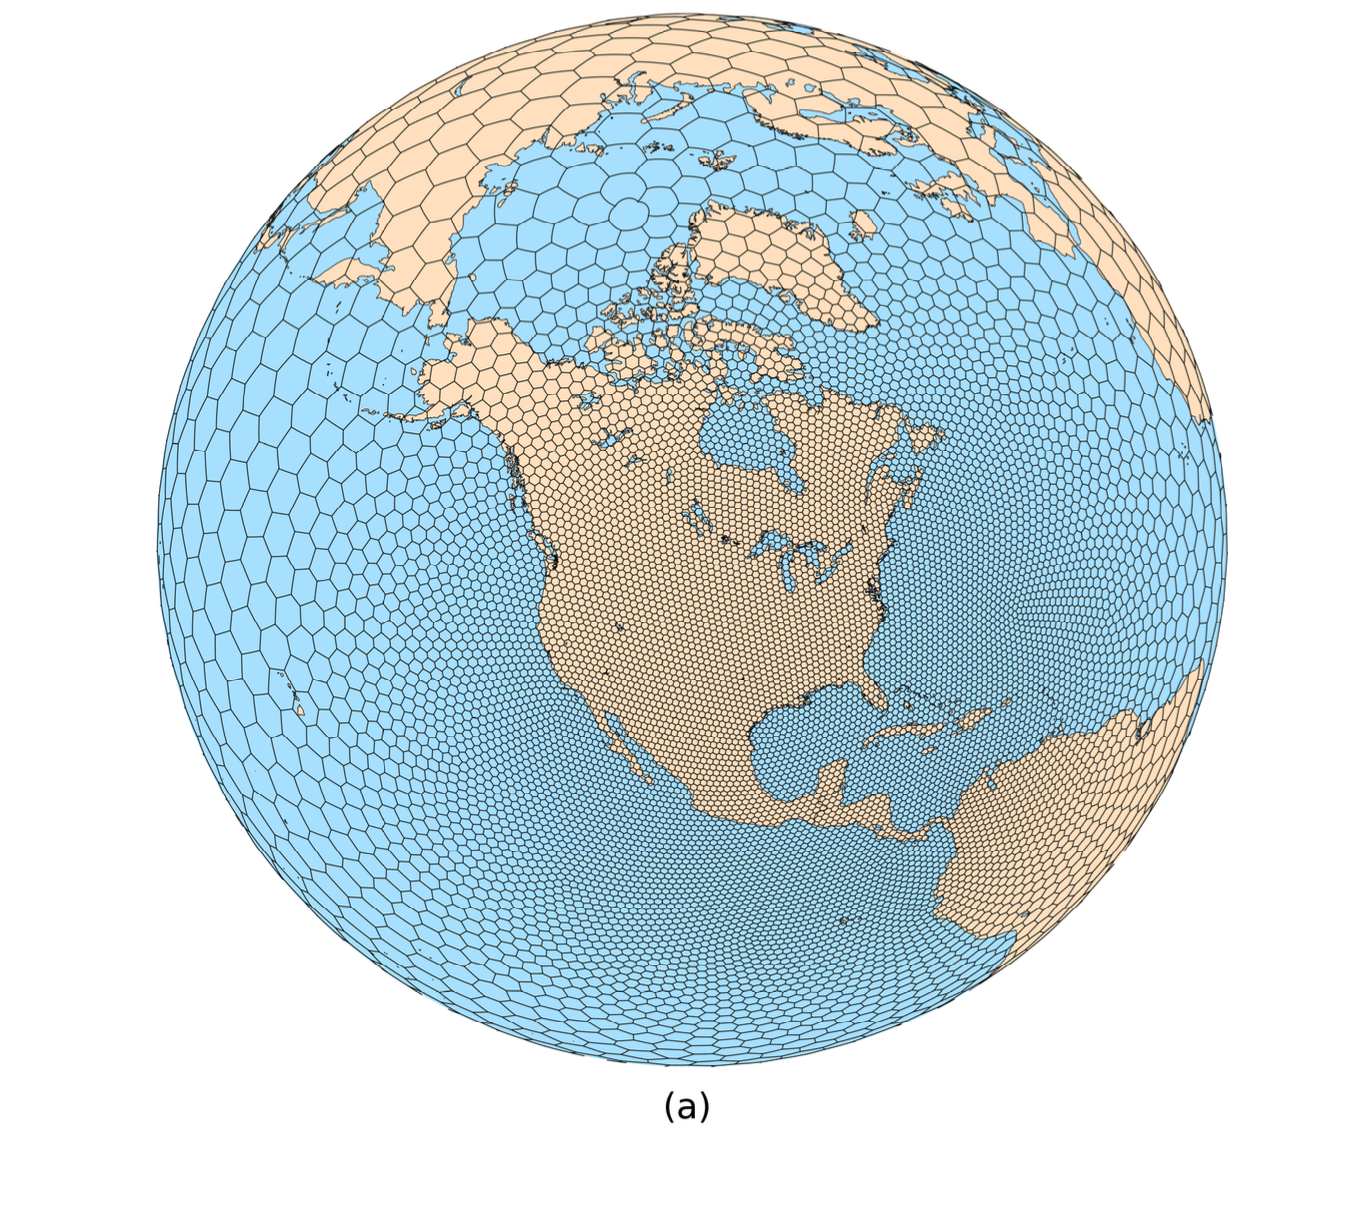
\includegraphics[width=0.7\textwidth, trim=10 70 10 0, clip]{docs/figuras/chapter3/ncl_plots_a.png} % Substitua pelo nome do seu arquivo
	\vspace{2mm}
	
	\centering 
	Source: \url{https://www2.mmm.ucar.edu/projects/mpas/site/visualization.html} (2025) .\par
	\label{fig:mpas-a} % Fonte centralizada
\end{figure}

\begin{figure}[htbp]
	\centering
	\caption{30km horizontal resolution at native mesh in MONAN.} 
	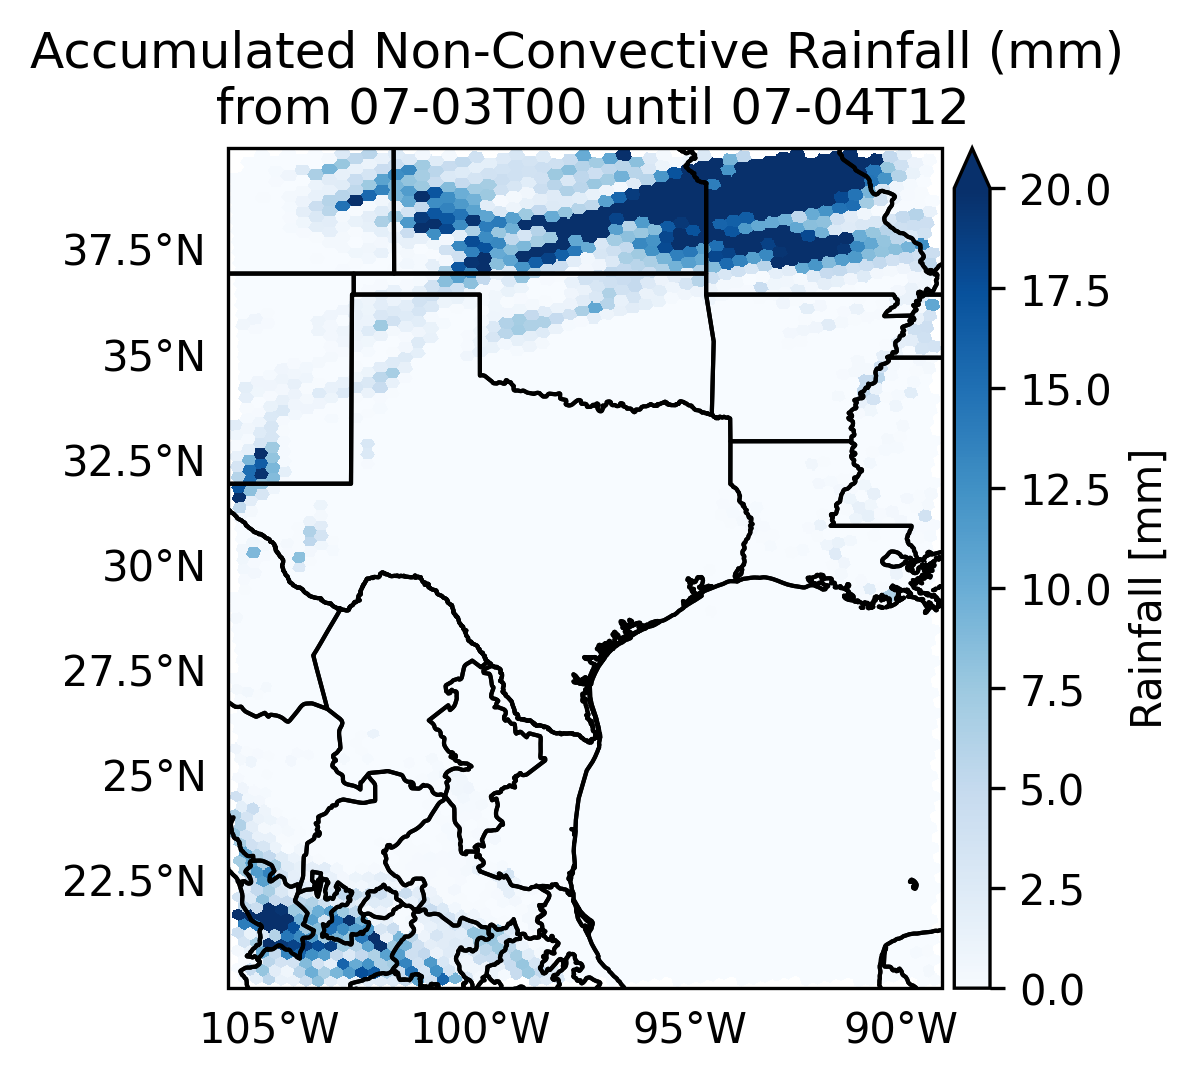
\includegraphics[width=0.7\textwidth, trim=0 0 0 0, clip]{docs/figuras/chapter3/rain_plot_native_grid.png} % Substitua pelo nome do seu arquivo
	\vspace{2mm}
	
	\centering 
	Source: Made by the author (2025) .\par
	\label{fig:non-convective rainfall} % Fonte centralizada
\end{figure}

As one can see, one of the big differences between MPAS and its predecessor, the WRF model, is that the model is discretized on centroidal Voronoi meshes using a C-grid staggering of the prognostic variables, allowing variable horizontal resolution, and also solving the equations of motion directly on these unstructured meshes \cite{skamarock2012multiscale}. 

For our study, a set of variables was chosen to perform it. Table \ref{tab:monan atmospheric variables} indicates the variable name inside MONAN, alongside with the long name and the unit.

\begin{table}[htbp]
	\centering
	\caption{MONAN Atmospheric Variables Selected for Model Evaluation}
	\vspace{2mm}
	\begin{tabular}{@{}lll@{}}
		\toprule
		\textbf{Variable name} & \textbf{Long name} & \textbf{Unit} \\
		\midrule
		rainc & Convective rainfall & mm/h \\
		rainnc & Not Convective rainfall & mm/h \\
		mslp & Mean sea level pressure & hPa \\
		wspd & Wind speed & m/s \\
		ctt & Cloud top temperature & °C \\
		\bottomrule
	\end{tabular}
	\label{tab:monan atmospheric variables}
	\vspace{2mm}
	
	{\centering Source: Made by the author, 2025.\par}
\end{table}

Total rainfall was computed by simply summing the variables rainnc and rainc for each lat/lon point. The wspd is the module of the squared sum of zonal and meridional winds at the first model level. From uzonal\_200hPa below, all variables are computed at the reference level pressure; for instance, uzona\_200hPa means the zonal wind at the pressure level of 200hPa.

\subsection{Initial condition generation}

To begin the integration process, Initial Conditions (IC) must be prepared by MPAS requirements, which can be found at the footnote of this page \footnote{\url{https://www2.mmm.ucar.edu/projects/mpas/site/documentation/users_guide/running.html}} \footnote{\url{https://www2.mmm.ucar.edu/projects/mpas/mpas_atmosphere_users_guide_7.0.pdf}}. We generated the initial conditions using the Weather Research \& Forecasting Model (WRF) Pre-Processing System (WPS), utilizing data obtained from ERA5, which we pre-processed with the WPS. These initial conditions were then uploaded into the MONAN IC folder and executed accordingly. For the IC sensitivity test, we also acquired a GRIB file from the Global Forecast System (GFS) model, a courtesy provided by Saulo R. Freitas, who already had the data available. The model will initially be set up with a global 30 km MPAS grid, with plans to modify this in future sections. It is important to note that a new IC will need to be created for each resolution.

\subsection{Post-processing}

Since the model output is generated on a non-structured grid, a post-processing step is necessary to map the native MPAS output to other meshes, enabling visualization on a standard lat/lon map. To achieve this, MONAN employs the convert-MPAS project \footnote{\url{https://github.com/mgduda/convert_mpas}}. This approach utilizes a nearest-neighbor scheme to remap integer fields to the target grid, with additional information available at this link.

In this study, the Climate Data Operators (CDO) were also utilized to remap various datasets, including ERA5, GPM-IMERG, GPM-MERGIR, and GSMaP, as well as several forecasts (such as those simulated at 15km and 60km horizontal resolutions) to the MONAN forecasts.

\chapter{METHODOLOGY: METRICS AND DIAGNOSTIC FIELDS}
\label{ch:methods}


%The analysis will focus on three main characteristics of cyclones commonly utilized \cite{deshpande2010impact, bopape2021sensitivity,  zarzycki2021metrics, nyongesa2024influence, mishra2024characteristics} in weather forecasting: track, intensity, and rainfall. The table below outlines the questions designed to guide the examination of each characteristic in alignment with the dissertation's objectives. This approach will help refine the metrics and outputs available in the existing literature.

Our methodology is designed based on three main characteristics of tropical cyclones commonly utilized in weather forecasting: track, intensity, and rainfall. The metrics that are currently used in similar studies will be described accordingly to each category. Then, for each hurricane, a table with addressed questions will be shown to guide the reader in the analysis and discussion of the results. This table will be part of the workflow, a diagram that shows the steps and figures/maps that will be created. 
All code made for this dissertation is available on the
\href{https://github.com/biancafusi/Dissertation}{GitHub - Dissertation Repository}, mainly written in Python.

%In the following subsections, the approaches and metrics used to evaluate each of these characteristics will be explained in detail. Finally, a workflow diagram will be presented, summarizing the described methods and indicating at which stage each question will be addressed.
%All code made for this dissertation is available on the git repository: \href{https://github.com/biancafusi/Dissertation}{GitHub - Dissertation Repository} mainly written in Python

\section{Trajectory}

A map illustrating the forecasted trajectories will be generated using a tracking algorithm developed by the author. A discussion regarding the performance of this tracking and guidance can be found in Appendix \ref{appendixB}. Additionally, a time series analysis will be conducted to evaluate the errors associated with each trajectory. These errors are defined as the distance between the central pressure reference points and the forecasted central pressure points, calculated using the GeoPy library\footnote{\href{https://geopy.readthedocs.io/en/stable/}{https://geopy.readthedocs.io/en/stable/}}. As noted in the literature, the calculations could be performed following the methodology proposed by \citeonline{moon2021five} but here we simply calculate the great-circle distance between two points. 

To quantitatively validate the results, a graphical representation will display the Mean Absolute Error (MAE) and Root Mean Square Error (RMSE) for each of the trajectories, regarding the reference dataset.

The MAE is widely employed \cite{ditchek2023improving, nyongesa2024influence} in the literature and can be defined as:

\begin{equation}
    \text{MAE} = \frac{1}{N}\sum_{i=1}^{N} |F_i -O_i|
\end{equation}

\noindent in this equation, $N$ represents the sample size (number of points in the trajectory), $F$ denotes the forecast outputs generated by the model, and $O$ refers to the observation outputs obtained from a reference dataset. The error values can range from 0 to $\infty$, with a perfect score indicated by 0. The aim is to calculate the average magnitude of the forecast errors. It is important to note that this error does not convey the direction of the deviations due to its absolute nature; this aspect will be examined using another method discussed later.

Along with the MAE, usually, RMSE is computed to seek a kind of average error, but now weighted according to the square of the error. As the same as before, it varies from 0 to $\infty$, and a perfect score means RMSE equal to 0. It is defined as:

\begin{equation}
    \text{RMSE} = \sqrt{\frac{1}{N}\sum_{i=1}^{N} (F_i -O_i)^2}
\end{equation}

The letters in this equation have the same meaning as in the previous equation. To better understand the potential trends in the trajectory, in addition to visual comparisons, one can utilize cross-track and along-track errors computed into a time series. The errors assess the deviation of the forecasted position from the observed path (cross-track) and the speed of the forecast from the observations (along-track). The cross-track error is measured perpendicularly to the observed trajectory, while the along-track error is measured along the actual course at a specified event. Together, these metrics\footnote{The equations used to compute those errors can be found at this website: \url{https://www.movable-type.co.uk/scripts/latlong.html}} can also indicate the directional error of each forecast. Figure~\ref{fig:cross-along-errors} more clearly illustrates the distinction between cross-track and along-track errors. 

\begin{figure}[htbp]
    \centering
    \caption{Illustration of cross-track and along-track errors. The definitions of Cross-Track Error (CTE) and Along-Track Error (ATE) are based on the distance between an observation (obs) and a forecast (fct) at the same valid time (T). This distance is computed as the great-circle distance.} % Título acima
    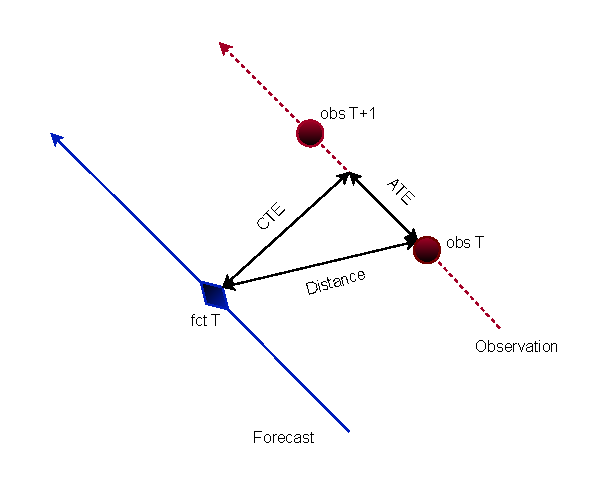
\includegraphics[width=0.8\textwidth]{docs/figuras/chapter4/cte_ate.pdf} 
    \label{fig:cross-along-errors}
    \vspace{0.5em}
    
    \centering
    Source: Made by the author (2025).
\end{figure}

In the context of our expected findings, negative (positive) values of cross-track errors indicate that the forecasted center of the hurricane is projected to be located to the west (east), while negative (positive) values of along-track errors suggest that the center is slower (faster) than its intended trajectory.

%Those errors can be clarified by examining the meteorological fields. Following the approach of \citeonline{gao2023regulating}, analyzing the 700 hPa geopotential height can reveal the large-scale features contributing to the bias in the trackings. For instance, in the authors' study, forecasts displaying significant eastward track bias for tropical cyclones often correspond with a noticeably weaker subtropical high over the North Atlantic. These fields can be computed easily using Python.

Such errors can be further investigated through the analysis of meteorological fields, as demonstrated by \citeonline{gao2023regulating}. For example, examining the 700 hPa geopotential height can help identify large-scale features that contribute to tracking biases. In their study, forecasts exhibiting a pronounced eastward track bias for tropical cyclones were often associated with a notably weaker subtropical high over the North Atlantic. Although this work does not include such an approach due to time constraints, it represents a different approach for future research and is highlighted here for reference.


In conclusion, utilizing a straightforward statistical mean of the errors (specifically the MAE and RMSE) can provide valuable insights into the overall performance of the MONAN simulations. The mean is defined as follows:

\begin{equation}
    \text{MEAN} = \frac{1}{E} \sum_{i=1}^{E} errors_i
\end{equation}

where E denotes the total number of experiments conducted using the MONAN framework. This approach facilitates a comprehensive understanding of the general behavior exhibited by the MONAN runs and can be compared with ERA5, for instance.

%%%%%%%%%%%%%%%%%%%%%%%%%%%%%%%%%%%%%%%%
\section{Intensity}

In reviewing the literature, tropical cyclone intensity is defined as the maximum surface wind speed associated with the central pressure \cite{demaria2007evaluation, landsea2013atlantic}. However, some studies argue that depending exclusively on wind speed does not fully capture the concept of intensity, suggesting that pressure can also serve as a significant indicator of forecasted intensity \cite{shepherd2017sensitivity, heming2017tropical}. This dissertation will adopt the latter approach by evaluating both pressure and wind as intensity indicators.

To conduct these evaluations, we will analyze time series data that includes the central pressure identified by the tracking system and the maximum wind speed, which is derived from the first level of the model. A discussion on how to determine this maximum wind speed in the model can be found in Appendix~\ref{appendixA}. The time series will serve as a measure of forecast performance, allowing us to assess how closely the computed values align with actual observations and where they occur.

In addition to a visual comparison, we will create a graph containing the MAE and RMSE to quantify the forecasts and rank them based on their effectiveness in illustrating intensity. Additionally, the mean of those errors can also be computed and compared with ERA5 to give us insights into the general MONAN performance. 

%To validate these results, we can examine meteorological fields such as the geopotential height between 850 hPa and 500 hPa, as well as the pressure and wind fields at 850 hPa, to gain insights into the forecast's impact on cyclone movement and intensity; all of the fields can easily be computed using Python. 

%%%%%%%%%%%%%%%%%%%%%%%%%%%%%%%%%%%%%%%%%%%
\section{Rainfall}

The analysis of rainfall for our runs is based on the methodology proposed by \citeonline{marchok2007validation}. According to these authors, evaluating forecasted rainfall requires examining three key aspects: the rainfall pattern, the mean and distribution of rain volume, and the extreme values.


To investigate the rainfall pattern, we will utilize the Equitable Threat Score (ETS; \citeonline{mesinger2008bias}) along with pattern correlation analysis (namely the Pearson Correlation Coefficient) and visual comparisons using selected snapshots, considering also the related bias of those fields. The mean and distribution of rain volume can be assessed through the computation of the Cumulative Density Function (CDF) and the Probability Density Function (PDF). Extreme rainfall values will be specifically analyzed by examining the 85th percentile computed at the CDF. Lastly, we will discuss a performance score for MONAN in comparison to ERA5 by averaging the results of all experiments. Table~\ref{tab:rainfall_metrics} summarizes the metrics to be computed, followed by a brief explanation of each metric and its intended purpose.

\begin{table}[H]
\centering
\caption{Metrics used to evaluate rainfall forecast performance}
\label{tab:rainfall_metrics}
\resizebox{\textwidth}{!}{
\begin{tabular}{lp{11cm}}
\toprule
\textbf{Metric} & \textbf{Definition} \\
\midrule
ETS (Equitable Threat Score) & Measures the skill of categorical forecasts by comparing the number of hits to what would be expected by chance:
\[
\text{ETS} = \frac{H - H_r}{H + F + M - H_r}
\]
where \(H\) is the number of hits, \(F\) is false alarms, \(M\) is misses, and \(H_r = \frac{(H+F)(H+M)}{total}\) is the expected number of hits due to chance. \\

Pearson Correlation Coefficient & Measures the spatial similarity between observed and forecasted rainfall fields:
\[
r = \frac{\sum_{i=1}^{n} (F_i - \bar{F})(O_i - \bar{O})}{\sqrt{\sum_{i=1}^{n} (F_i - \bar{F})^2 \sum_{i=1}^{n} (O_i - \bar{O})^2}}
\]
where \(F\) and \(O\) are forecasted and observed values, calculated over $n$ data points, where $i$ is the index running from 1 to $n$. \\

Bias & Quantifies the difference between forecast and observation:
\[
\text{Bias} = F - O
\] \\

CDF (Cumulative Distribution Function) & Represents the probability that a variable takes a value less than or equal to a given threshold:
\[
\text{CDF}(x) = P(X \leq x)
\] \\

PDF (Probability Density Function) & Describes the relative likelihood for a variable to take a specific value:
\[
\text{PDF}(x) = \frac{d}{dx} \, \text{CDF}(x)
\] \\
\bottomrule
\end{tabular}
}

\vspace{2mm}
{\centering Source: Made by the author (2025).\par}

\end{table}


The ETS evaluates how well forecasted “yes” events correspond to observed “yes” events, while accounting for agreements due to random chance. According to \citeonline{marchok2007validation}, this implies that the ETS penalizes a model for overproducing rainfall above a given threshold, even if the rainfall pattern is realistic. For this metric, a hit is defined as an event that was forecasted to occur and did occur; a miss is an event that was not forecasted but occurred; and a false alarm is an event that was forecasted but did not occur.

Pattern correlation is computed as the Pearson correlation coefficient (r) between the forecasted and observed rainfall fields. The correlation ranges from -1 to 1, where: ($i$) $r = 1$ indicates a perfect positive linear relationship; ($ii$) $r = -1$, a perfect negative linear relationship; and ($iii$) $r = 0$ implies no linear relationship between forecast and observation.

The bias is the difference between the forecast ($F$) and the observations ($O$), typically averaged over time or space. A negative bias indicates underestimation, while a positive bias indicates overestimation. The bias can range from negative to positive infinity, with 0 representing a perfect forecast.

Both the CDF and the PDF will be used to analyze rainfall distributions. The CDF shows the cumulative probability of rainfall values up to a certain threshold. For example, the corresponding x-axis value when the y-axis equals to 0.5 (or 50\%) on the CDF corresponds to the median rainfall amount. The CDF ranges from 0 to 1 on the y-axis, indicating the proportion of the data below a given threshold on the x-axis. For instance, the 0.85 mark on the CDF corresponds to the 85th percentile, meaning 85\% of the data falls below that threshold, and the remaining 15\% above it. This is a straightforward way to seek for rainfall extremes.

The PDF, similar to a histogram, describes the probability of observing values within a specific range. It is normalized such that the total area under the curve equals 1. To interpret the PDF, one can compute the area under the curve within a specified range, which represents the probability of a value falling in that interval. Mathematically, the CDF is the integral of the PDF. One should notice that both CDF and PDF can be computed empirically or theoretically. The difference between them is that when computing empirically, one will consider the natural distribution of data, and theoretically, one will consider a mathematical distribution (gamma, Gaussian, etc). In this study, we will utilize the empirical approach.



%%%%%%%%%%%%%%%%%%%%%%%%%%%%%%%%%%%%%%%%%%%%%
\section{Hurricane Beryl workflow}

With the hurricane Beryl event, the goal is to investigate the cold pool parameterization alongside sensitivity tests, and with those sensitivity tests, select an optimal parameter configuration for the parameterization. 

The table below outlines the questions designed to guide the examination of each characteristic in alignment with the dissertation's objectives. This approach will help refine the discussion and outputs available in the existing literature.

\begin{table}[H]
	\centering
	\caption{Key Research Questions for Track, Intensity, and Rainfall Assessment}
	\label{tab:research_questions}
	\resizebox{\textwidth}{!}{
		\begin{tabular}{lp{11cm}l}
			\toprule
			\textbf{Topic} & \textbf{Question} & \textbf{ID} \\
			\midrule
			\multirow{6}{*}{Trajectory} 
			& What is the overall performance of the parameterization and sensitivity tests in reproducing the hurricane's track? & T.1 \\
			& What is the error (in kilometers) associated with these tracks? & T.2 \\
			& Which configuration shows the best performance? & T.3 \\
			& After how many forecast hours do larger deviations begin to appear? & T.4 \\
			& Is there any observable trend in the tracks? & T.5 \\
			& What is the overall performance of MONAN? & T.6 \\
			\midrule
			\multirow{4}{*}{Intensity} 
			& What is the overall performance of the parameterization and sensitivity tests in reproducing the hurricane's intensity? & I.1 \\
			& How much bias is present in these results? & I.2 \\
			& How well does ERA5 perform in reproducing this intensity, and why? & I.3 \\
			& What is the overall performance of MONAN? & I.4 \\
			\midrule
			\multirow{7}{*}{Rainfall} 
			& What is the overall performance of the parameterization and sensitivity tests in reproducing the hurricane’s rainfall pattern? & R.1 \\
			& In which regions is there a negative (or positive) bias in the rainfall field? & R.2 \\
			& What is the overall performance of the parameterization and sensitivity tests in reproducing the hurricane’s cloud morphology? & R.3 \\
			& How much light, moderate, and heavy rainfall is being produced by the simulations? & R.4 \\
			& What is the average rainfall produced by the simulations? & R.5 \\
			& What is the bias between the extreme rainfall produced by the simulations and the reference data? & R.6 \\
			& What is the overall performance of MONAN? & R.7 \\
			\bottomrule
		\end{tabular}
	}
	\label{tab:questions}
	
	\vspace{2mm}
	{\centering Source: Made by the author (2025).\par}
	
\end{table}

The workflow below summarizes and organizes the upcoming steps. After a quick initial analysis, the results will be visually represented as trapezoidal shapes, while discussions will be depicted with rectangular shapes. This distinction helps clarify the types of information being presented at each stage of the process. Following this, the boxes containing question IDs, as outlined in Table\ref{tab:questions}, related to the three aspects under evaluation (trajectory, intensity, and rainfall) will be also displayed in the workflow.

\begin{figure}[p]
    \centering
    \caption{Workflow Overview of Hurricane Berryl}
    \label{fig:workflow}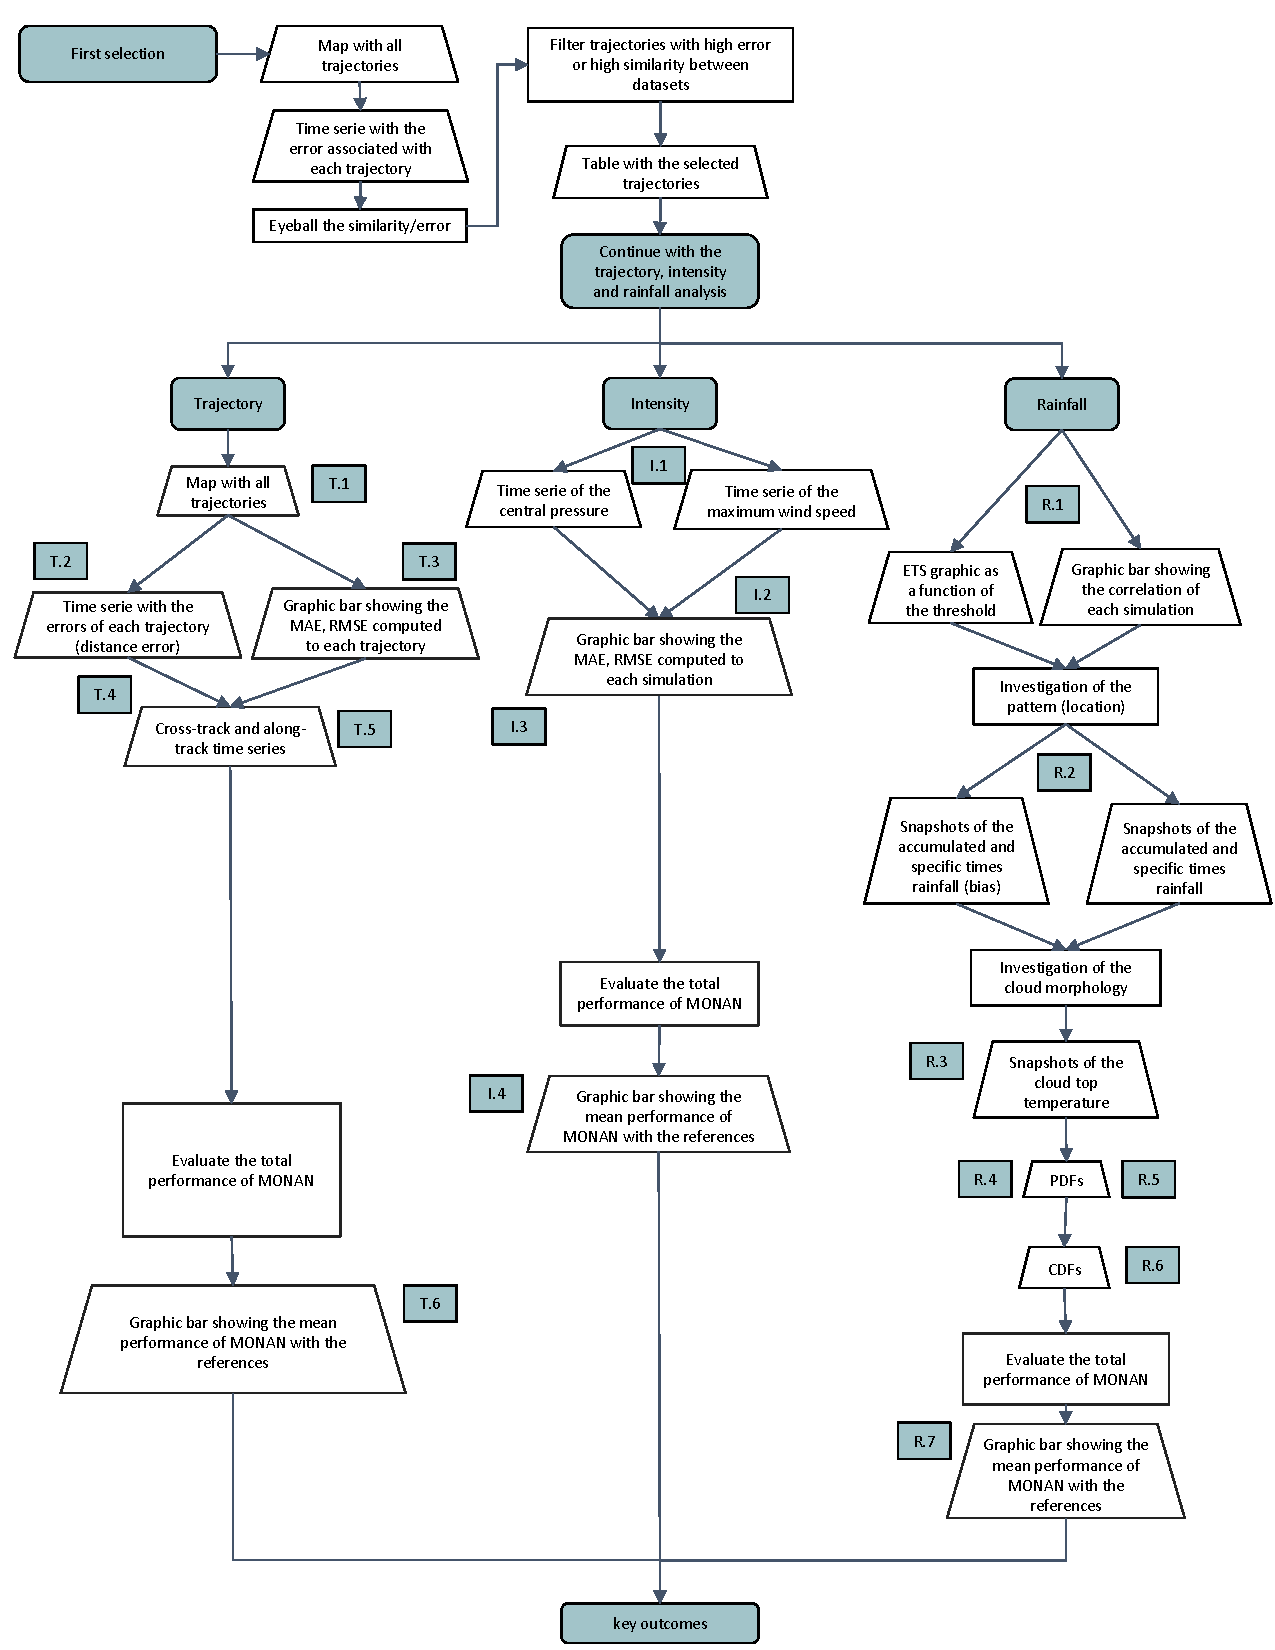
\includegraphics[width=\textwidth,height=\textheight,keepaspectratio]{docs/figuras/chapter4/BERYL_worflow_01.pdf}

    \vspace{0.5em}
    
    \centering
    Source: Made by the author (2025).
\end{figure}

The reader should note that an initial selection of the results will be conducted. As the diagram indicates, a trajectory map will be created, accompanied by distance errors. The selection criteria will focus on experiments that do not contribute significantly to the discussion, either because they are part of a set of similar experiments or due to excessively large errors that do not accurately represent the model state we aim to address.

\section{Hurricane Helene workflow}

Now we aim to test the best configuration alongside the cold pool effect and the highest resolution effect in another hurricane, Helene. Table \ref{tab:questions2} indicates the questions addressed for this investigation and futhermore, a similiar diagram as designed in the previous section were made here.

\begin{table}[H]
	\centering
	\caption{Key Research Questions for Track, Intensity, and Rainfall Assessment}
	\label{tab:research_questions_v2}
	\resizebox{\textwidth}{!}{
		\begin{tabular}{lp{11cm}l}
			\toprule
			\textbf{Topic} & \textbf{Question} & \textbf{ID} \\
			\midrule
			\multirow{4}{*}{Trajectory} 
			& What is the overall performance of the optimal configuration found, the parameterization, and the high-resolution effect in reproducing the hurricane's track? & T.1 \\
			& What is the error (in kilometers) associated with these tracks? & T.2 \\
			& After how many forecast hours do larger deviations begin to appear? & T.3 \\
			& Is there any observable trend in the tracks? & T.4 \\
			\midrule
			\multirow{2}{*}{Intensity} 
			& What is the overall performance of the optimal configuration found, the parameterization, and the high-resolution effect in reproducing the hurricane's intensity? & I.1 \\
			& How much bias is present in these results? & I.2 \\
			\midrule
			\multirow{6}{*}{Rainfall} 
			& What is the overall performance of the optimal configuration found, the parameterization, and the high-resolution effect in reproducing the hurricane’s rainfall pattern? & R.1 \\
			& In which regions is there a negative (or positive) bias in the rainfall field? & R.2 \\
			& What is the overall performance of the optimal configuration found, the parameterization, and the high-resolution effect in reproducing the hurricane’s cloud morphology? & R.3 \\
			& How much light, moderate, and heavy rainfall is being produced by the simulations? & R.4 \\
			& What is the average rainfall produced by the simulations? & R.5 \\
			& What is the bias between the extreme rainfall produced by the simulations and the reference data? Do the forecasts capture the extreme event in North Carolina? & R.6 \\
			\bottomrule
		\end{tabular}
	}
	\label{tab:questions2}
	
	\vspace{2mm}
	{\centering Source: Made by the author (2025).\par}
	
\end{table}

\begin{figure}[p]
	\centering
	\caption{Workflow Overview of Hurricane Helene}
	\label{fig:workflow}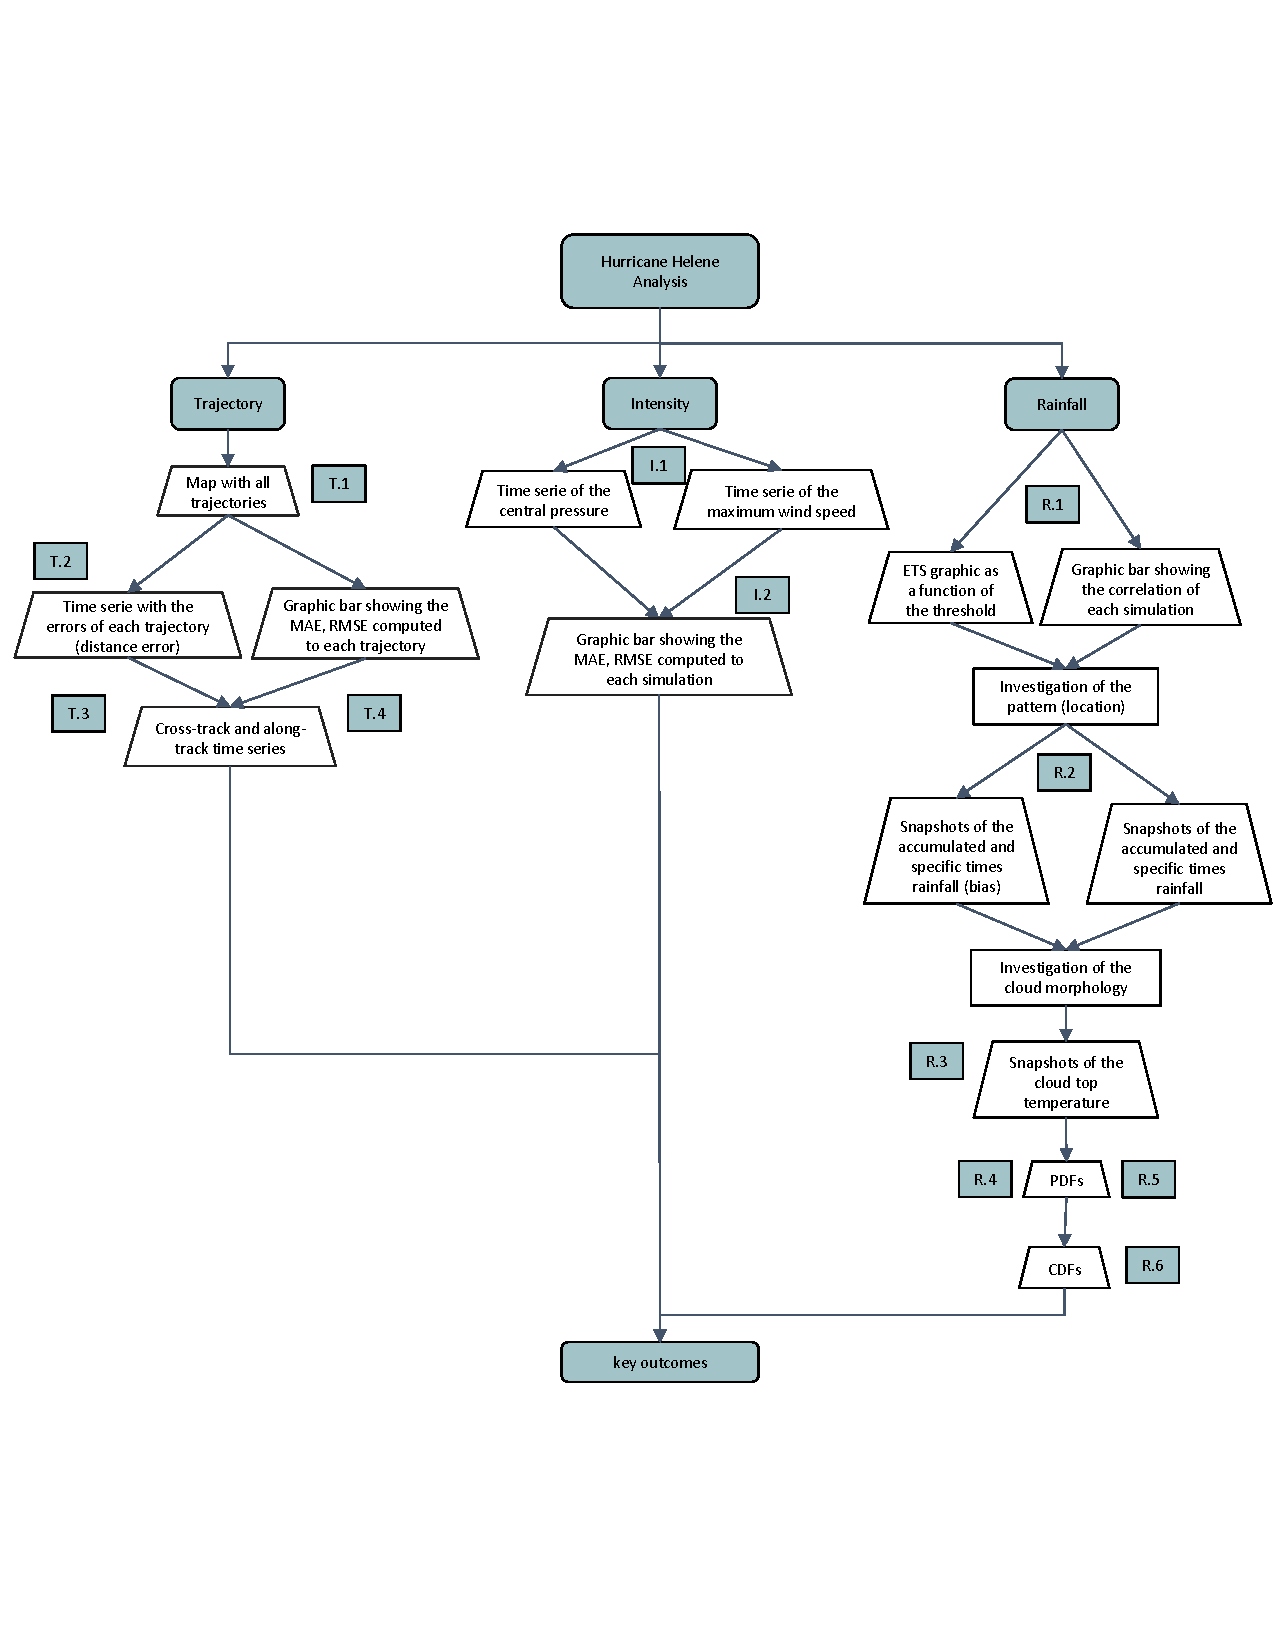
\includegraphics[width=\textwidth,height=\textheight,keepaspectratio]{docs/figuras/chapter4/HELENE_workflow_02.pdf}
	
	\vspace{0.5em}
	
	\centering
	Source: Made by the author (2025).
\end{figure}




 %% 4o capítulo
%%%%%%%%%%%%%%%%%%%%%%%%%%%%%%%%%%%%%%%%%%%%%%%%%%%%%%%%%%%%%%%%%%%%%%%%%%%%%%%

\chapter{CASE STUDY: HURRICANE BERYL}
\label{ch:beryl}

This chapter explores the results of implementing cold pool parameterization in the latest Brazilian numerical weather and climate prediction model, MONAN. It emphasizes the model's performance in predicting hurricane trajectory, intensity, and rainfall, using Hurricane Beryl as a case study, which occurred between June and July 2024 in the North Atlantic Basin. Following a brief introduction to the event, the chapter presents the results of the forecast and offers a direct comparison between ERA5 and MONAN. Finally, a discussion section will address the questions outlined previously in Table \ref{tab:questions}.
% VISTO

\section{Event description - hurricane Beryl}

Hurricane Beryl formed in the deep tropical Atlantic’s Main Development Region on June 28th, forming a tropical depression near 1200 UTC 28 June about 1200 nautical miles \footnote{In North American meteorology, it is common to use: pressure in millibars (mb), where 1 mb = 1 hPa; distance in nautical miles (nm), where 1 nm = 1.852 km; wind speed in knots (kt), where 1 kt = 1.852 km/h; and precipitation in inches (in), where 1 inch = 25.4 mm} east of Barbados, with a center at 1007 mb and wind speed of 30 kts. According to reports from the National Oceanic and Atmospheric Administration (NOAA), the storm rapidly intensified into a major hurricane, moving eastward and ultimately reaching Category 5 on the Saffir-Simpson Hurricane Wind Scale, making it the earliest Category 5 hurricane on record in the Atlantic Basin. Figure \ref{fig:hurricanepath} display all the trajectory computed with the best track dataset.

\begin{figure}[h!]
	\centering
	\caption{2024 Hurricane path according to best track analysis}
	\label{fig:hurricanepath}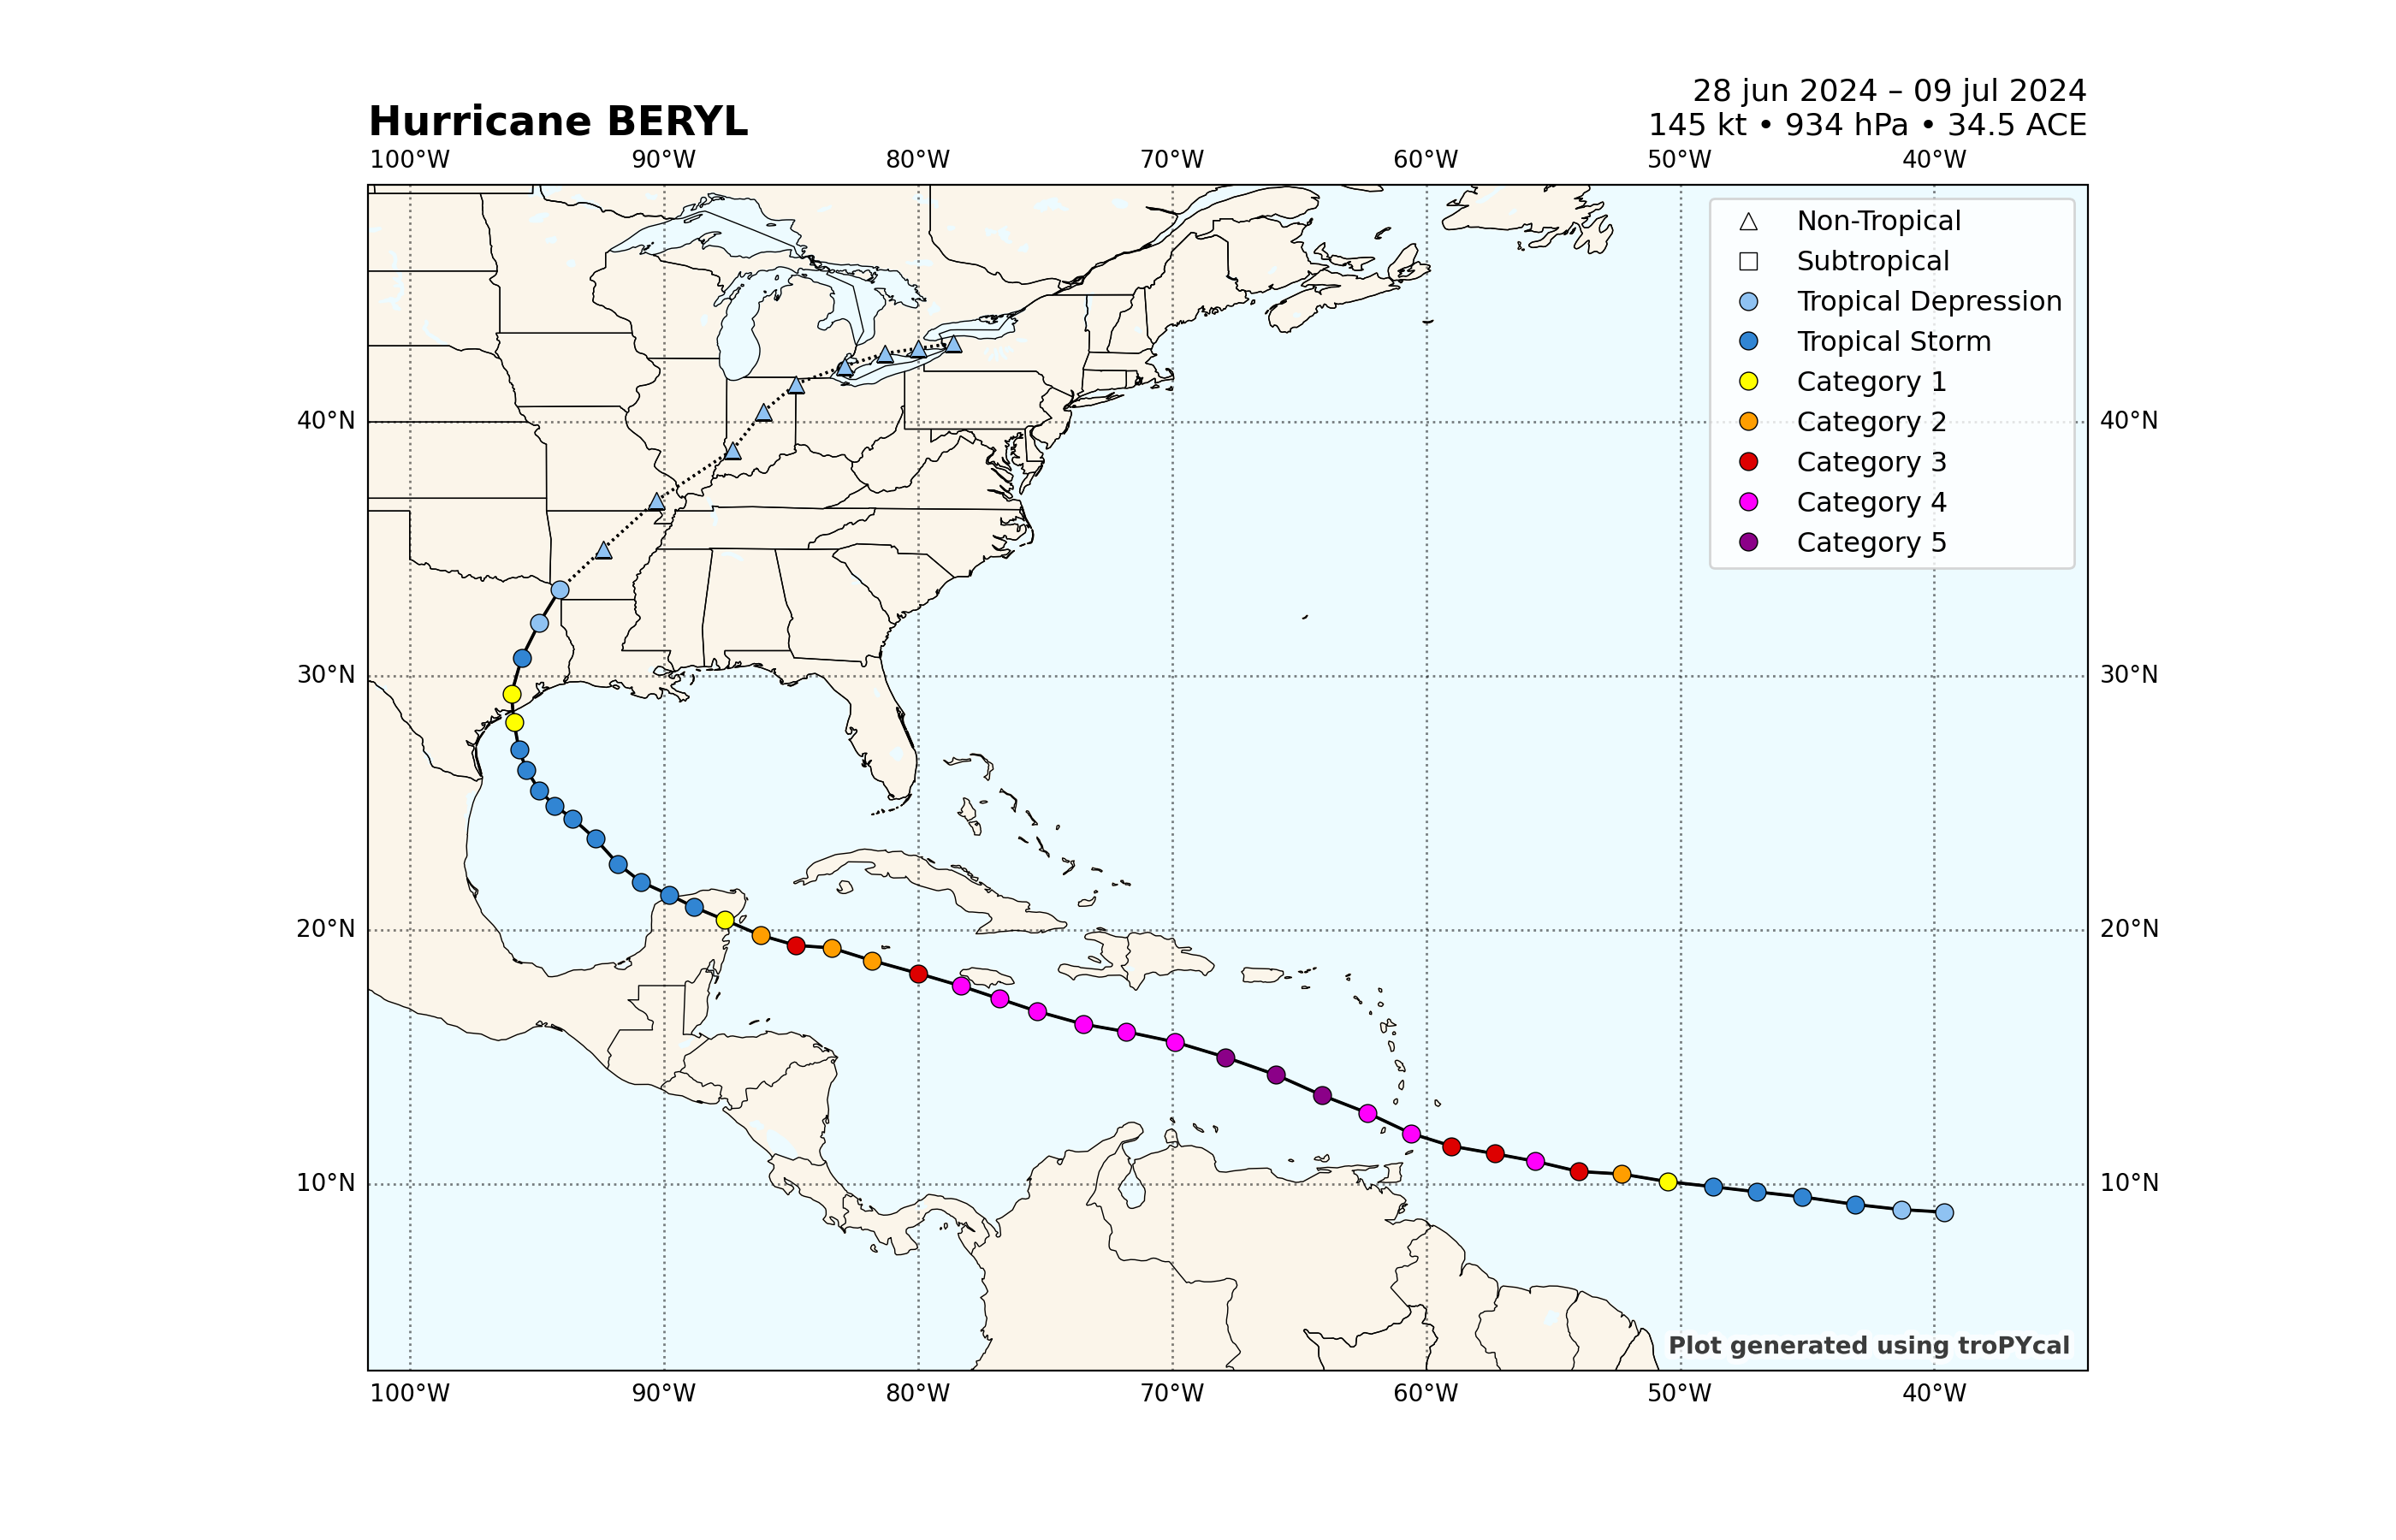
\includegraphics[width=\textwidth,height=\textheight,keepaspectratio]{docs/figuras/chapter5/beryl_2024.png}
	\centering
	Source: Made by the author (2025).
\end{figure}

It is important to note that the figure presented in the upper-right quadrant indicates critical meteorological parameters, including the peak wind speed recorded at 145 knots, the minimum mean sea level pressure of 934 hPa, and the Accumulated Cyclone Energy (ACE), which is quantified at 34.5. These values are derived directly from the best track dataset.

The first landfall of Hurricane Beryl occurred on the island of Carriacou in Grenada as a high-end Category 4 storm on July 1st, subsequently intensifying to a Category 5 in the Eastern Caribbean Sea. From a disaster perspective, the total damages in the Grenada Region are significant, with estimates of approximately US\$ 218.0 million, which accounts for about 16.5 percent of the GDP for 2023 \cite{gunasekera2024global}. Satellite images illustrating the hurricane's transition from Category 4 to Category 5, passing through the first landfall, are presented in Figure \ref{fig:HurricaneBerylBand13}.

\begin{figure}[h!]
	\centering
	\caption{Hurricane Beryl view from the GEOCOLOR composite (left) and Band 13 (right) when passing through the first landfall}
	
	\begin{minipage}{.48\textwidth}
		\centering
		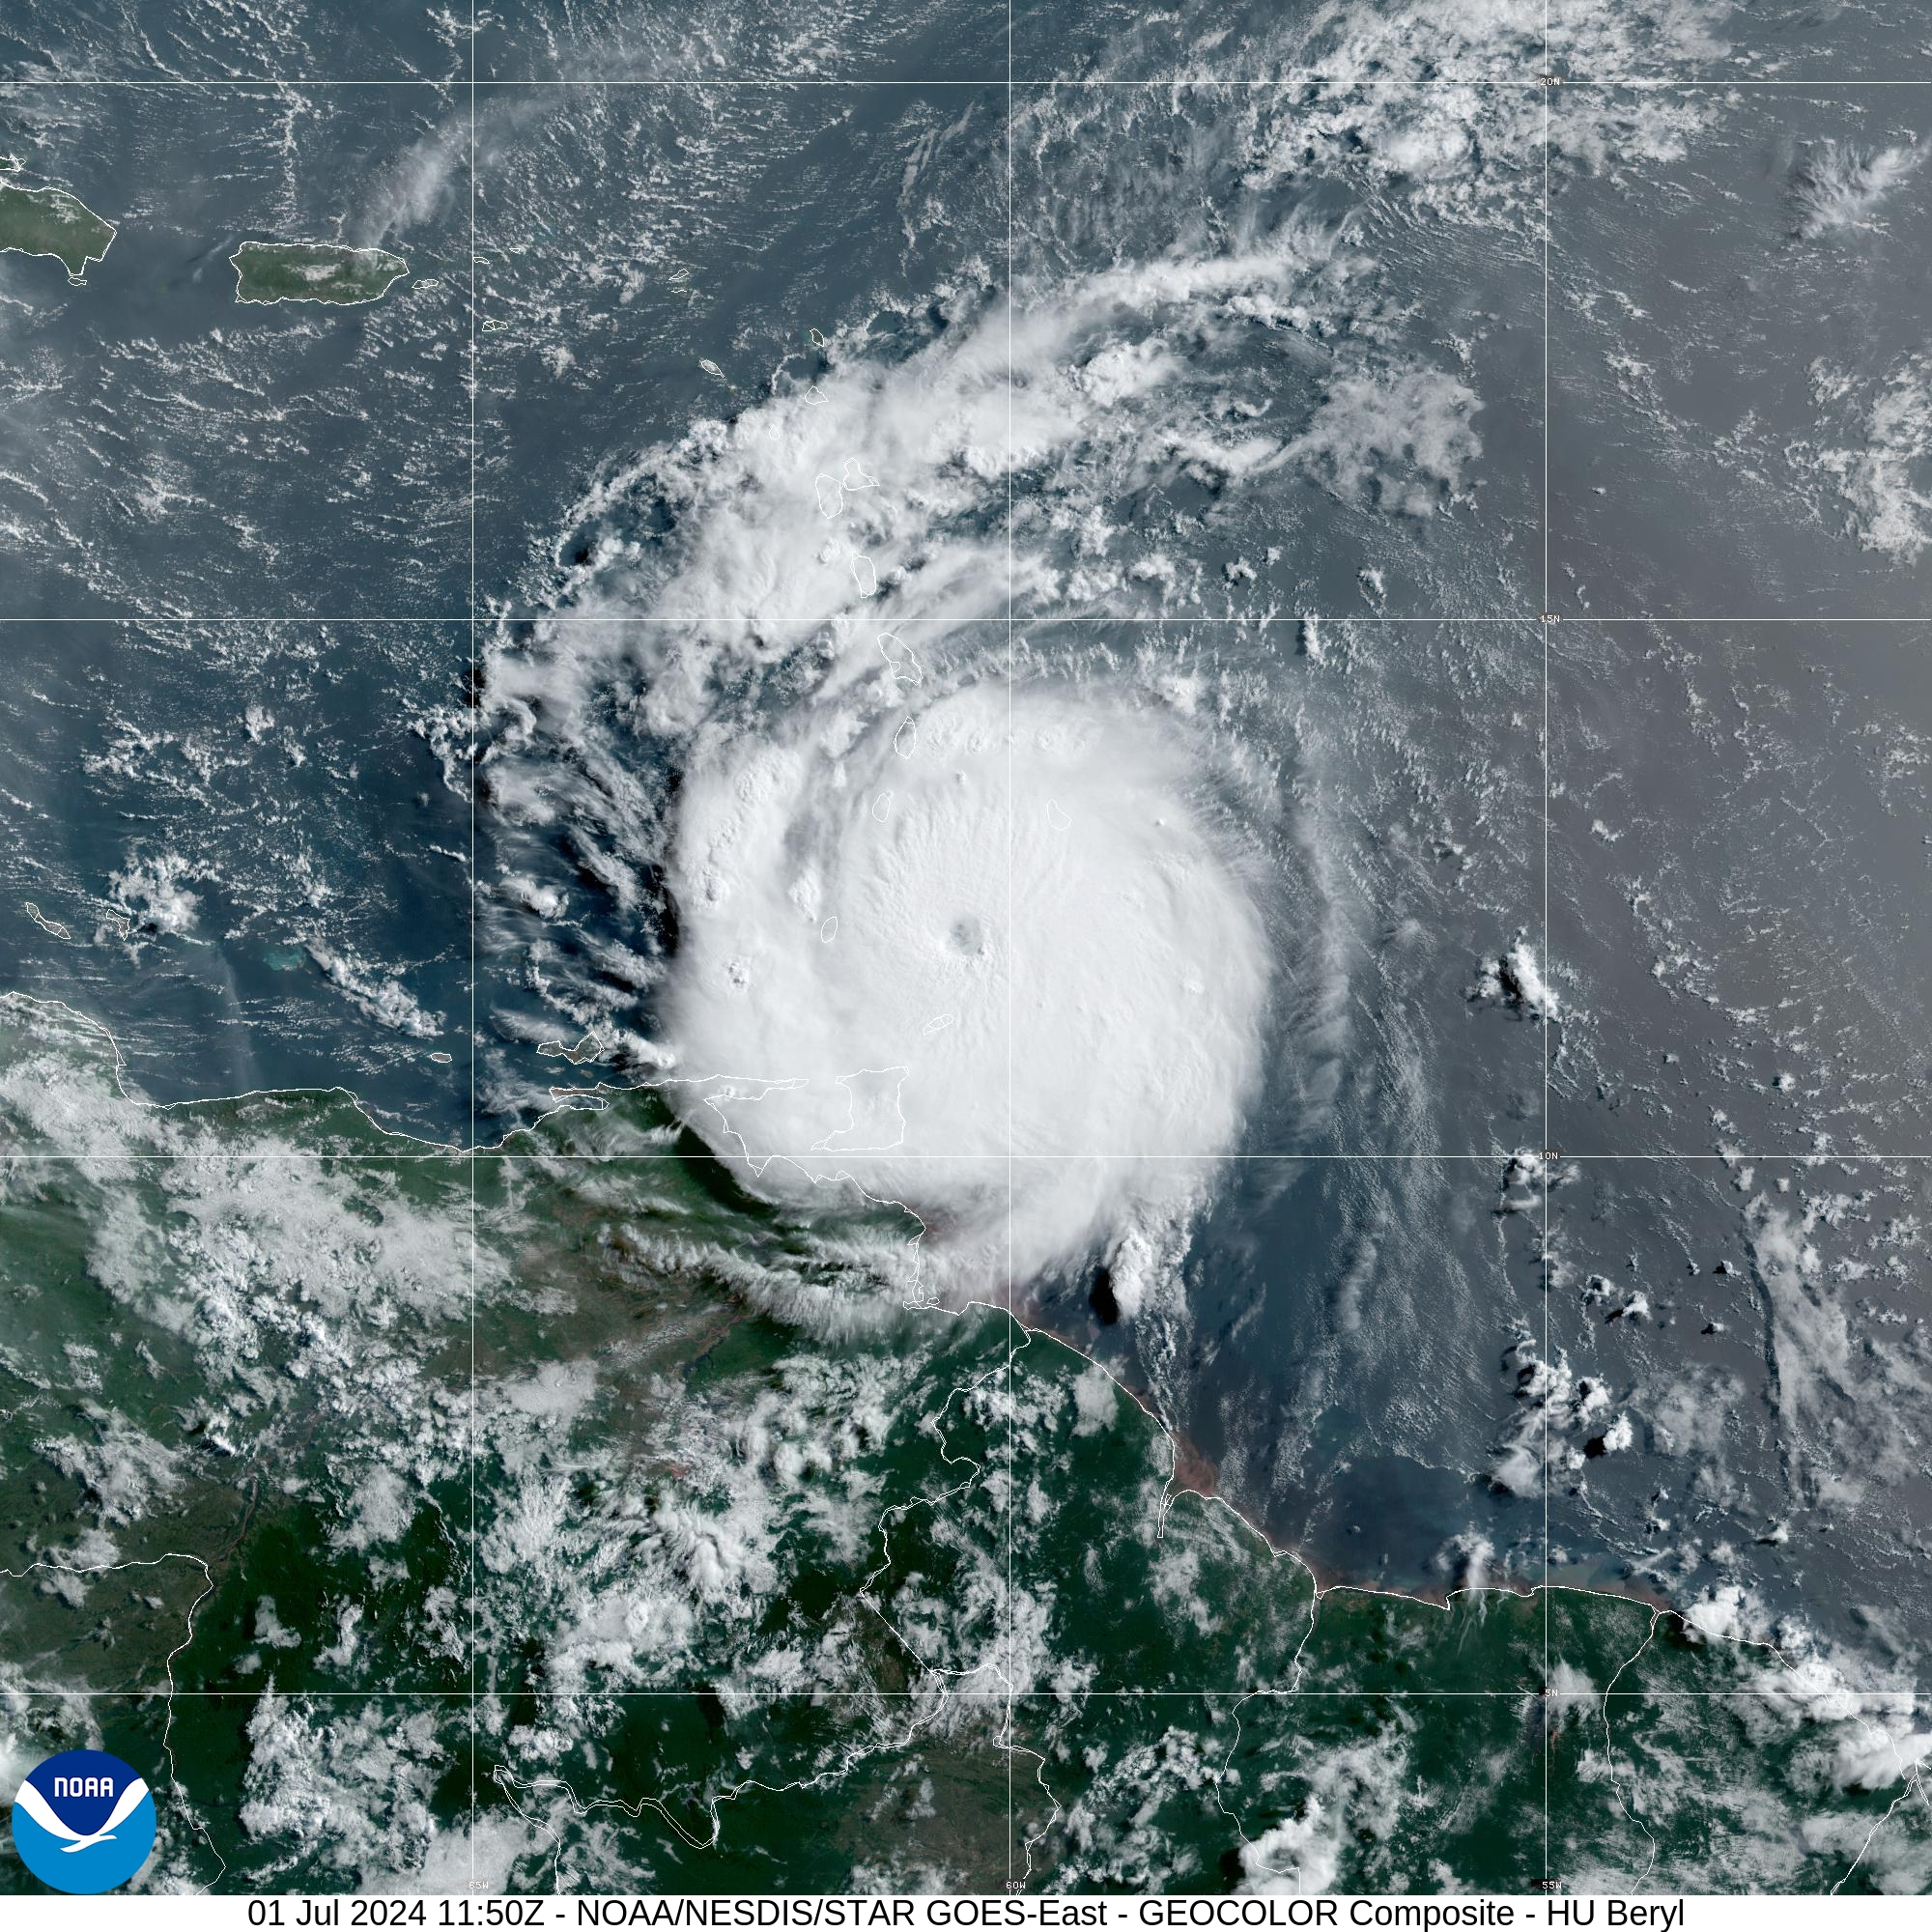
\includegraphics[width=\linewidth]{docs/figuras/chapter5/20241831150_GOES16-ABI-FL-GEOCOLOR-AL022024-2000x2000.jpg}
		\label{}
	\end{minipage}%
	\hfill
	\begin{minipage}{.48\textwidth}
		\centering
		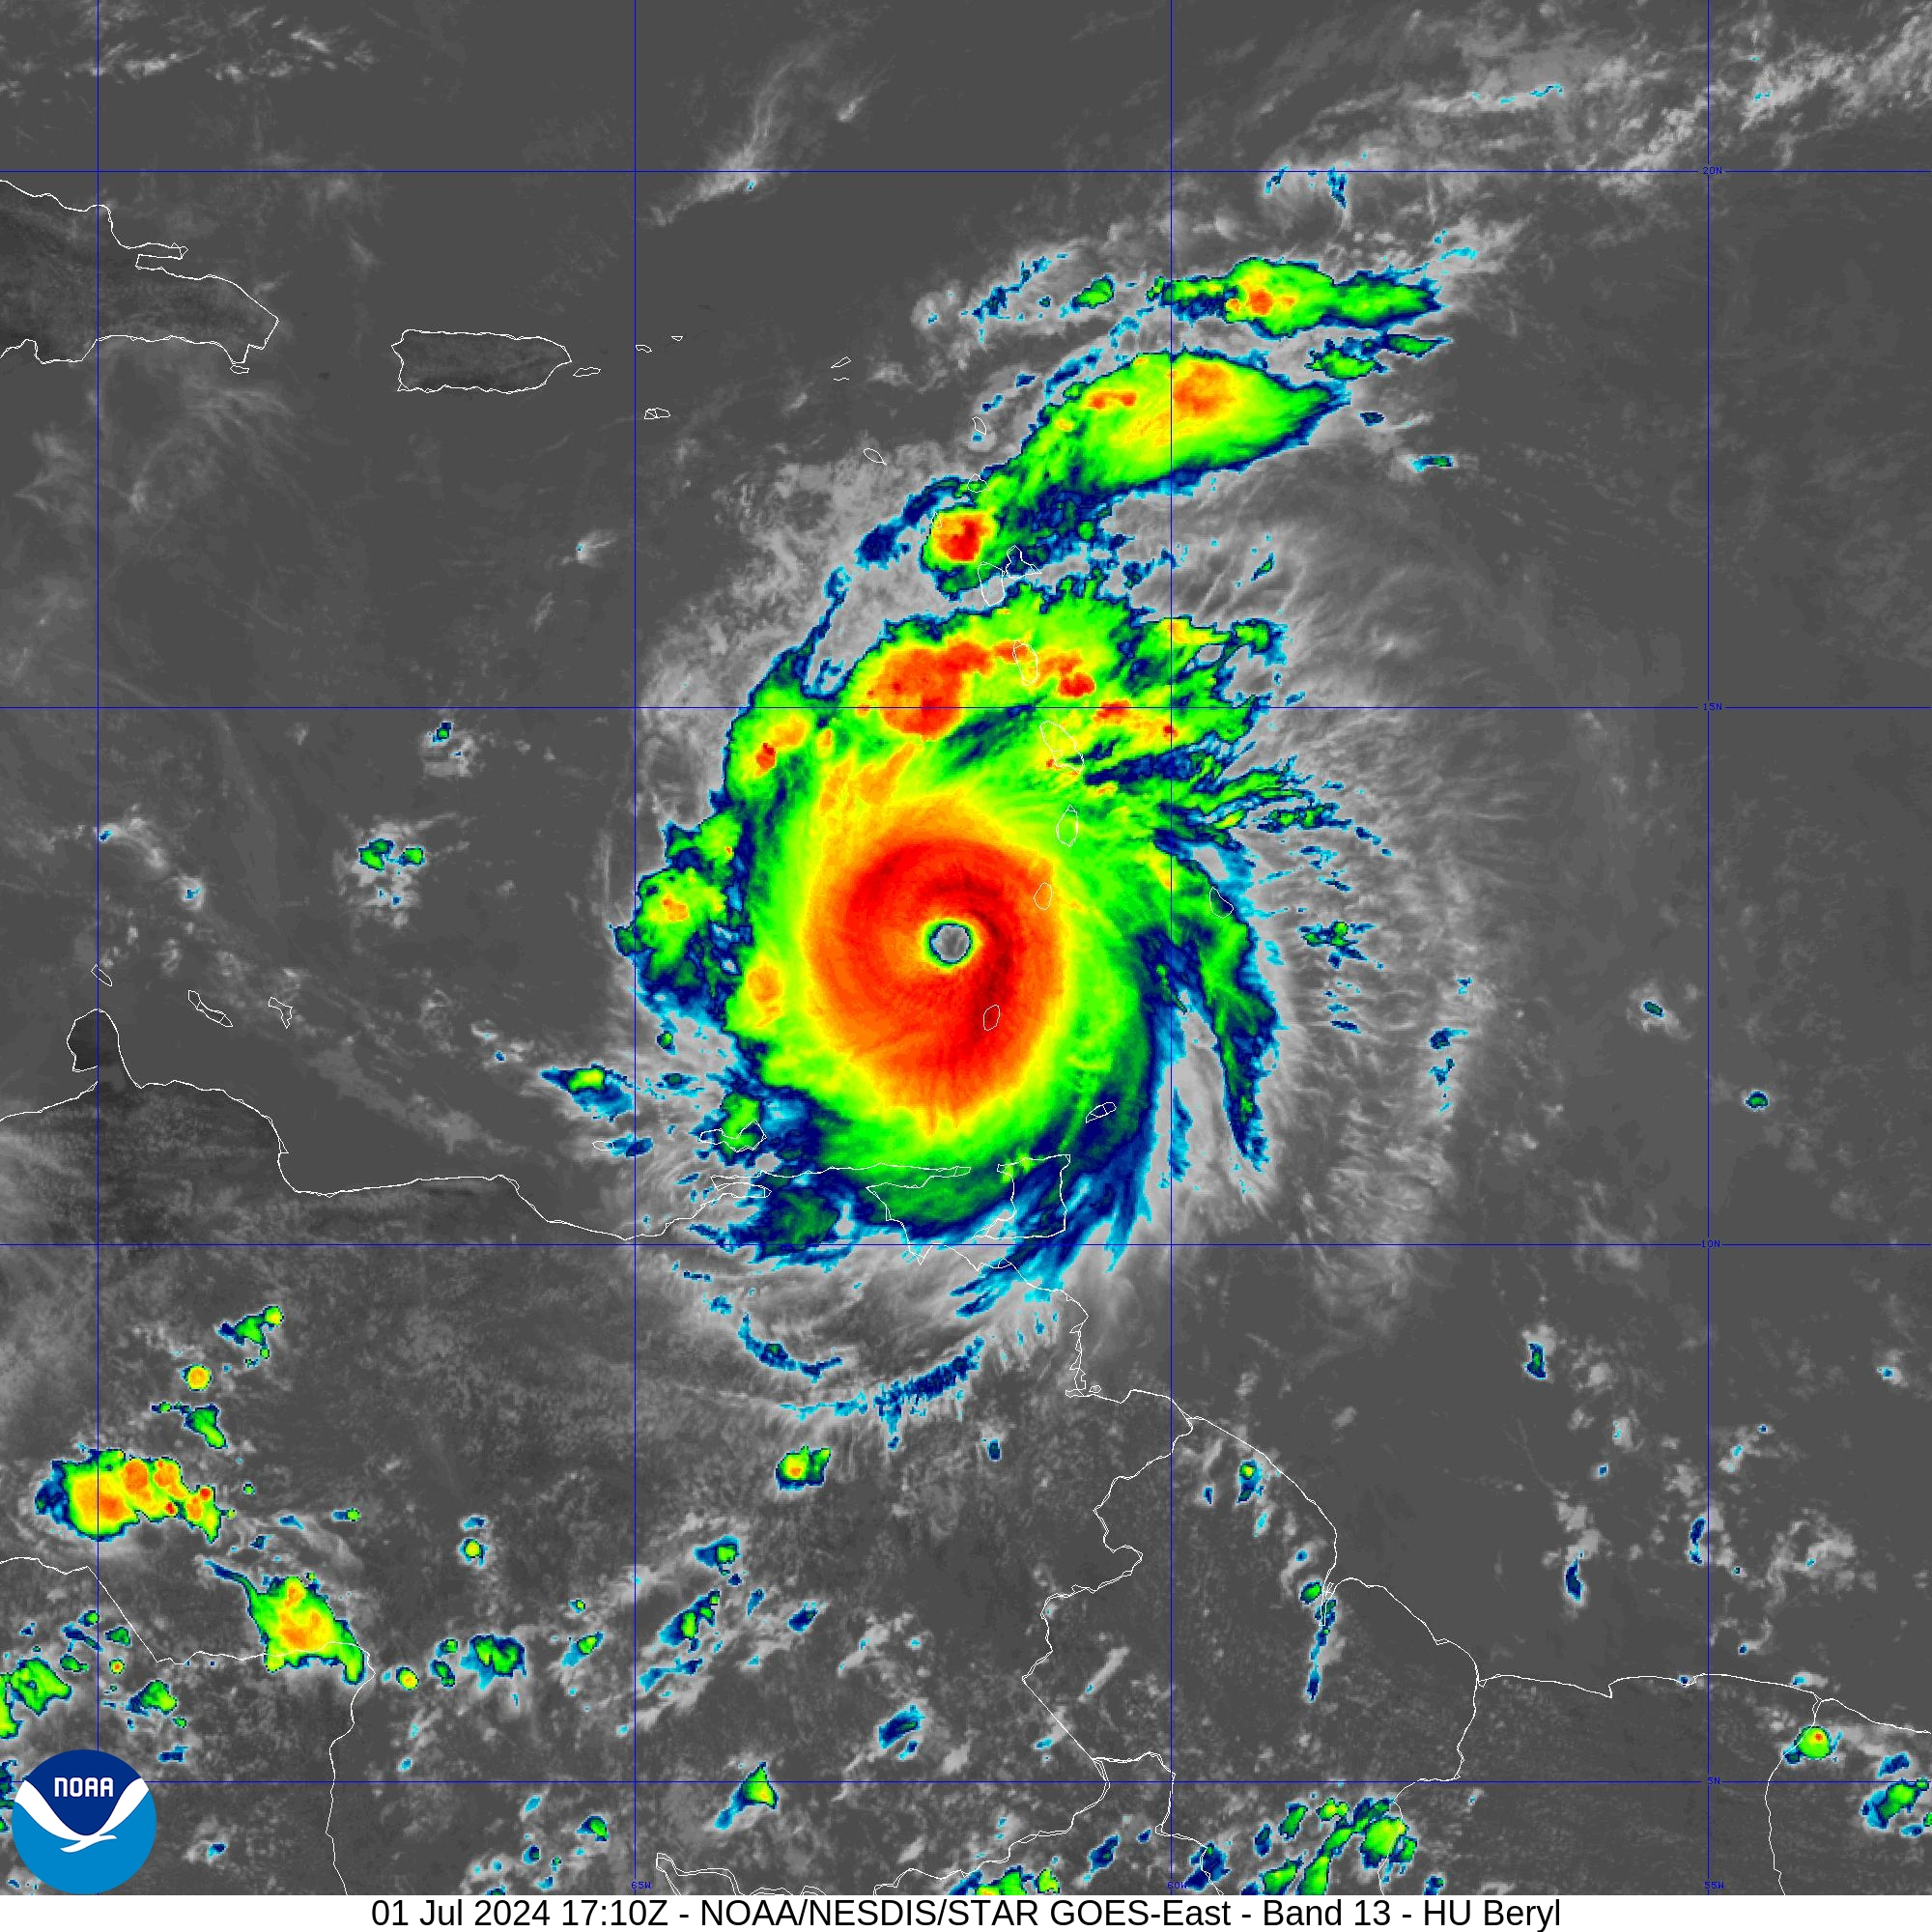
\includegraphics[width=\linewidth]{docs/figuras/chapter5/20241831710_GOES16-ABI-FL-13-AL022024-2000x2000.jpg}
		\label{fig:HurricaneBerylBand13}
	\end{minipage}
Source: \url{https://www.star.nesdis.noaa.gov/star/index.php.}
\end{figure}

At the passage through the Caribbean region, the rainfall was more intense in Jamaica, with widespread totals between 8 to 12 inches, and a peak of 13.62 inches observed at Knockpatrick in Manchester Parish, representing the highest storm-total rainfall reported.

The storm began to weaken before making a second landfall on the Yucatán Peninsula as a high-end Category 2 hurricane early on July 5th. Following its passage through the Peninsula, the hurricane continued to weaken while moving northwest, influenced by a large mid to upper-level trough of low pressure over the Central U.S., which eroded the robust ridge of high pressure over the Gulf of Mexico \cite{li2025generative}. The combination of increasing wind shear and dry air entrainment maintained a nearly steady state until dawn on July 7th. Later that morning, Hurricane Beryl progressed toward the Central Texas coast (northwest) as the mid to upper-level trough deepened to the north. An influx of moisture and decreased wind shear allowed the storm to become better organized, resulting in it being classified as a Category 1 hurricane by 11 PM CDT on July 7th (04:00 UTC on July 8th). A glimpse of this large scale environment is shown at Figure \ref{fig:mlsp}.

\begin{figure}[h!]
	\centering
	\caption{500 mb Geopotential Height and MSLP at July 8th, 00:00 UTC}
	\label{fig:mlsp}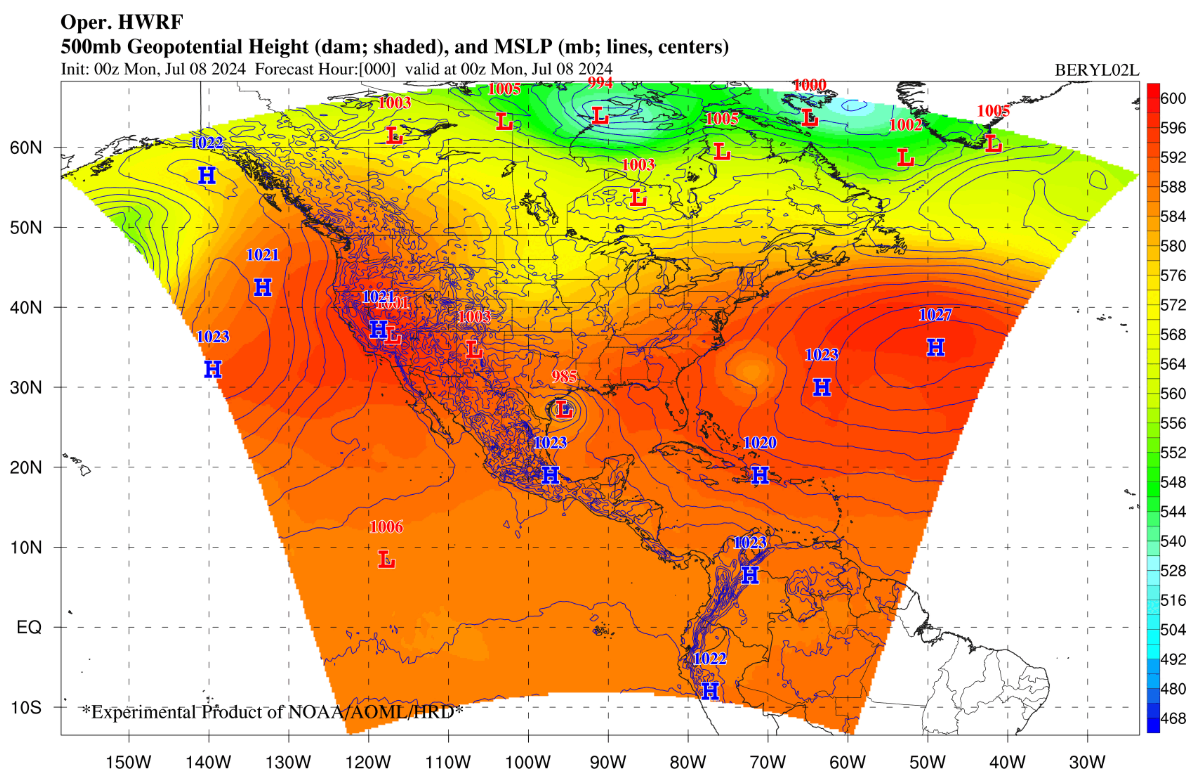
\includegraphics[width=\textwidth,height=\textheight,keepaspectratio]{docs/figuras/chapter5/beryl02l.png}
	\centering
	Source: \url{https://storm.aoml.noaa.gov/viewer/?projectName=BASIN}.
\end{figure}

At approximately 4 AM CDT on July 8th (09:00 UTC on July 8th), the hurricane made landfall near Matagorda along the Texas coast. Its maximum sustained winds were about 129 km/h (80 mph), and its minimum central pressure was 979 hPa. Figure 3 shows satellite and radar imagery capturing Hurricane Beryl's approach to the Texas coast.

\begin{figure}[h!]
	\centering
	\caption{HB view from NEXRAD (top) and GEOCOLOR composite (bottom) when reaching the Texas Coast.}
	\label{fig:nexradgeocolor}
	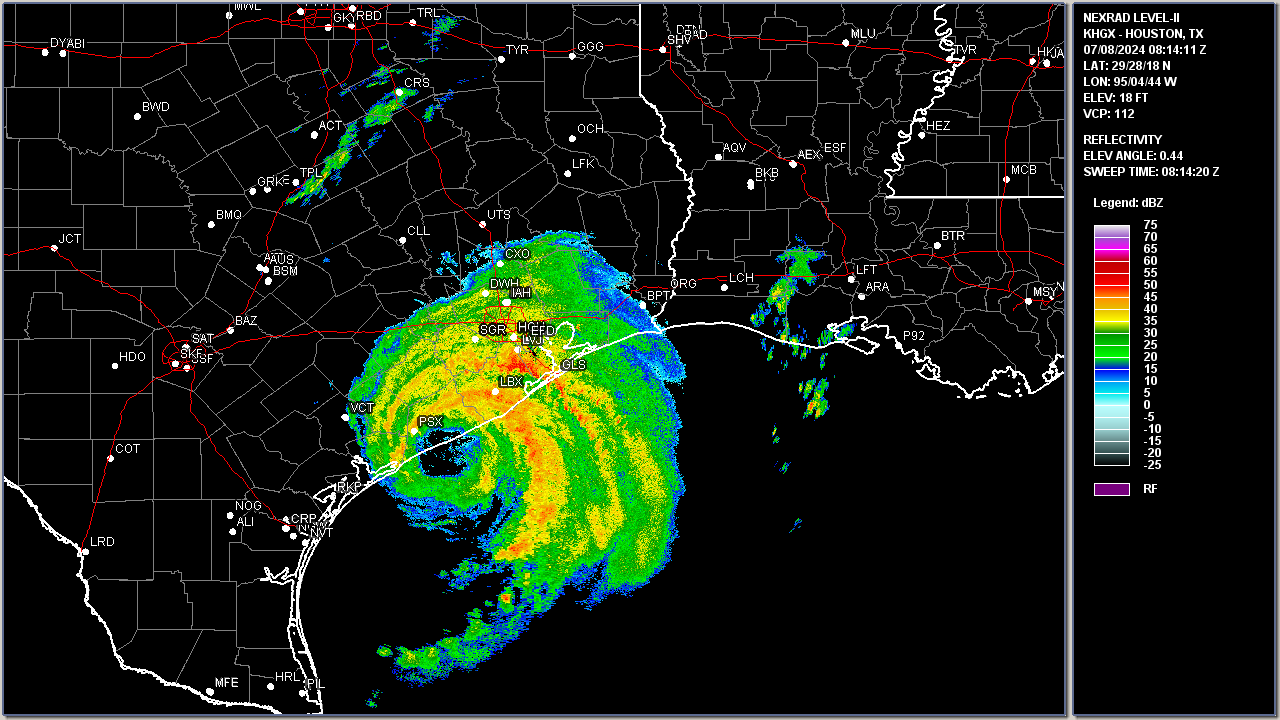
\includegraphics[width=0.8\textwidth]{docs/figuras/chapter5/20240708-0814Z-HGX.png}
	\vspace{3mm}
	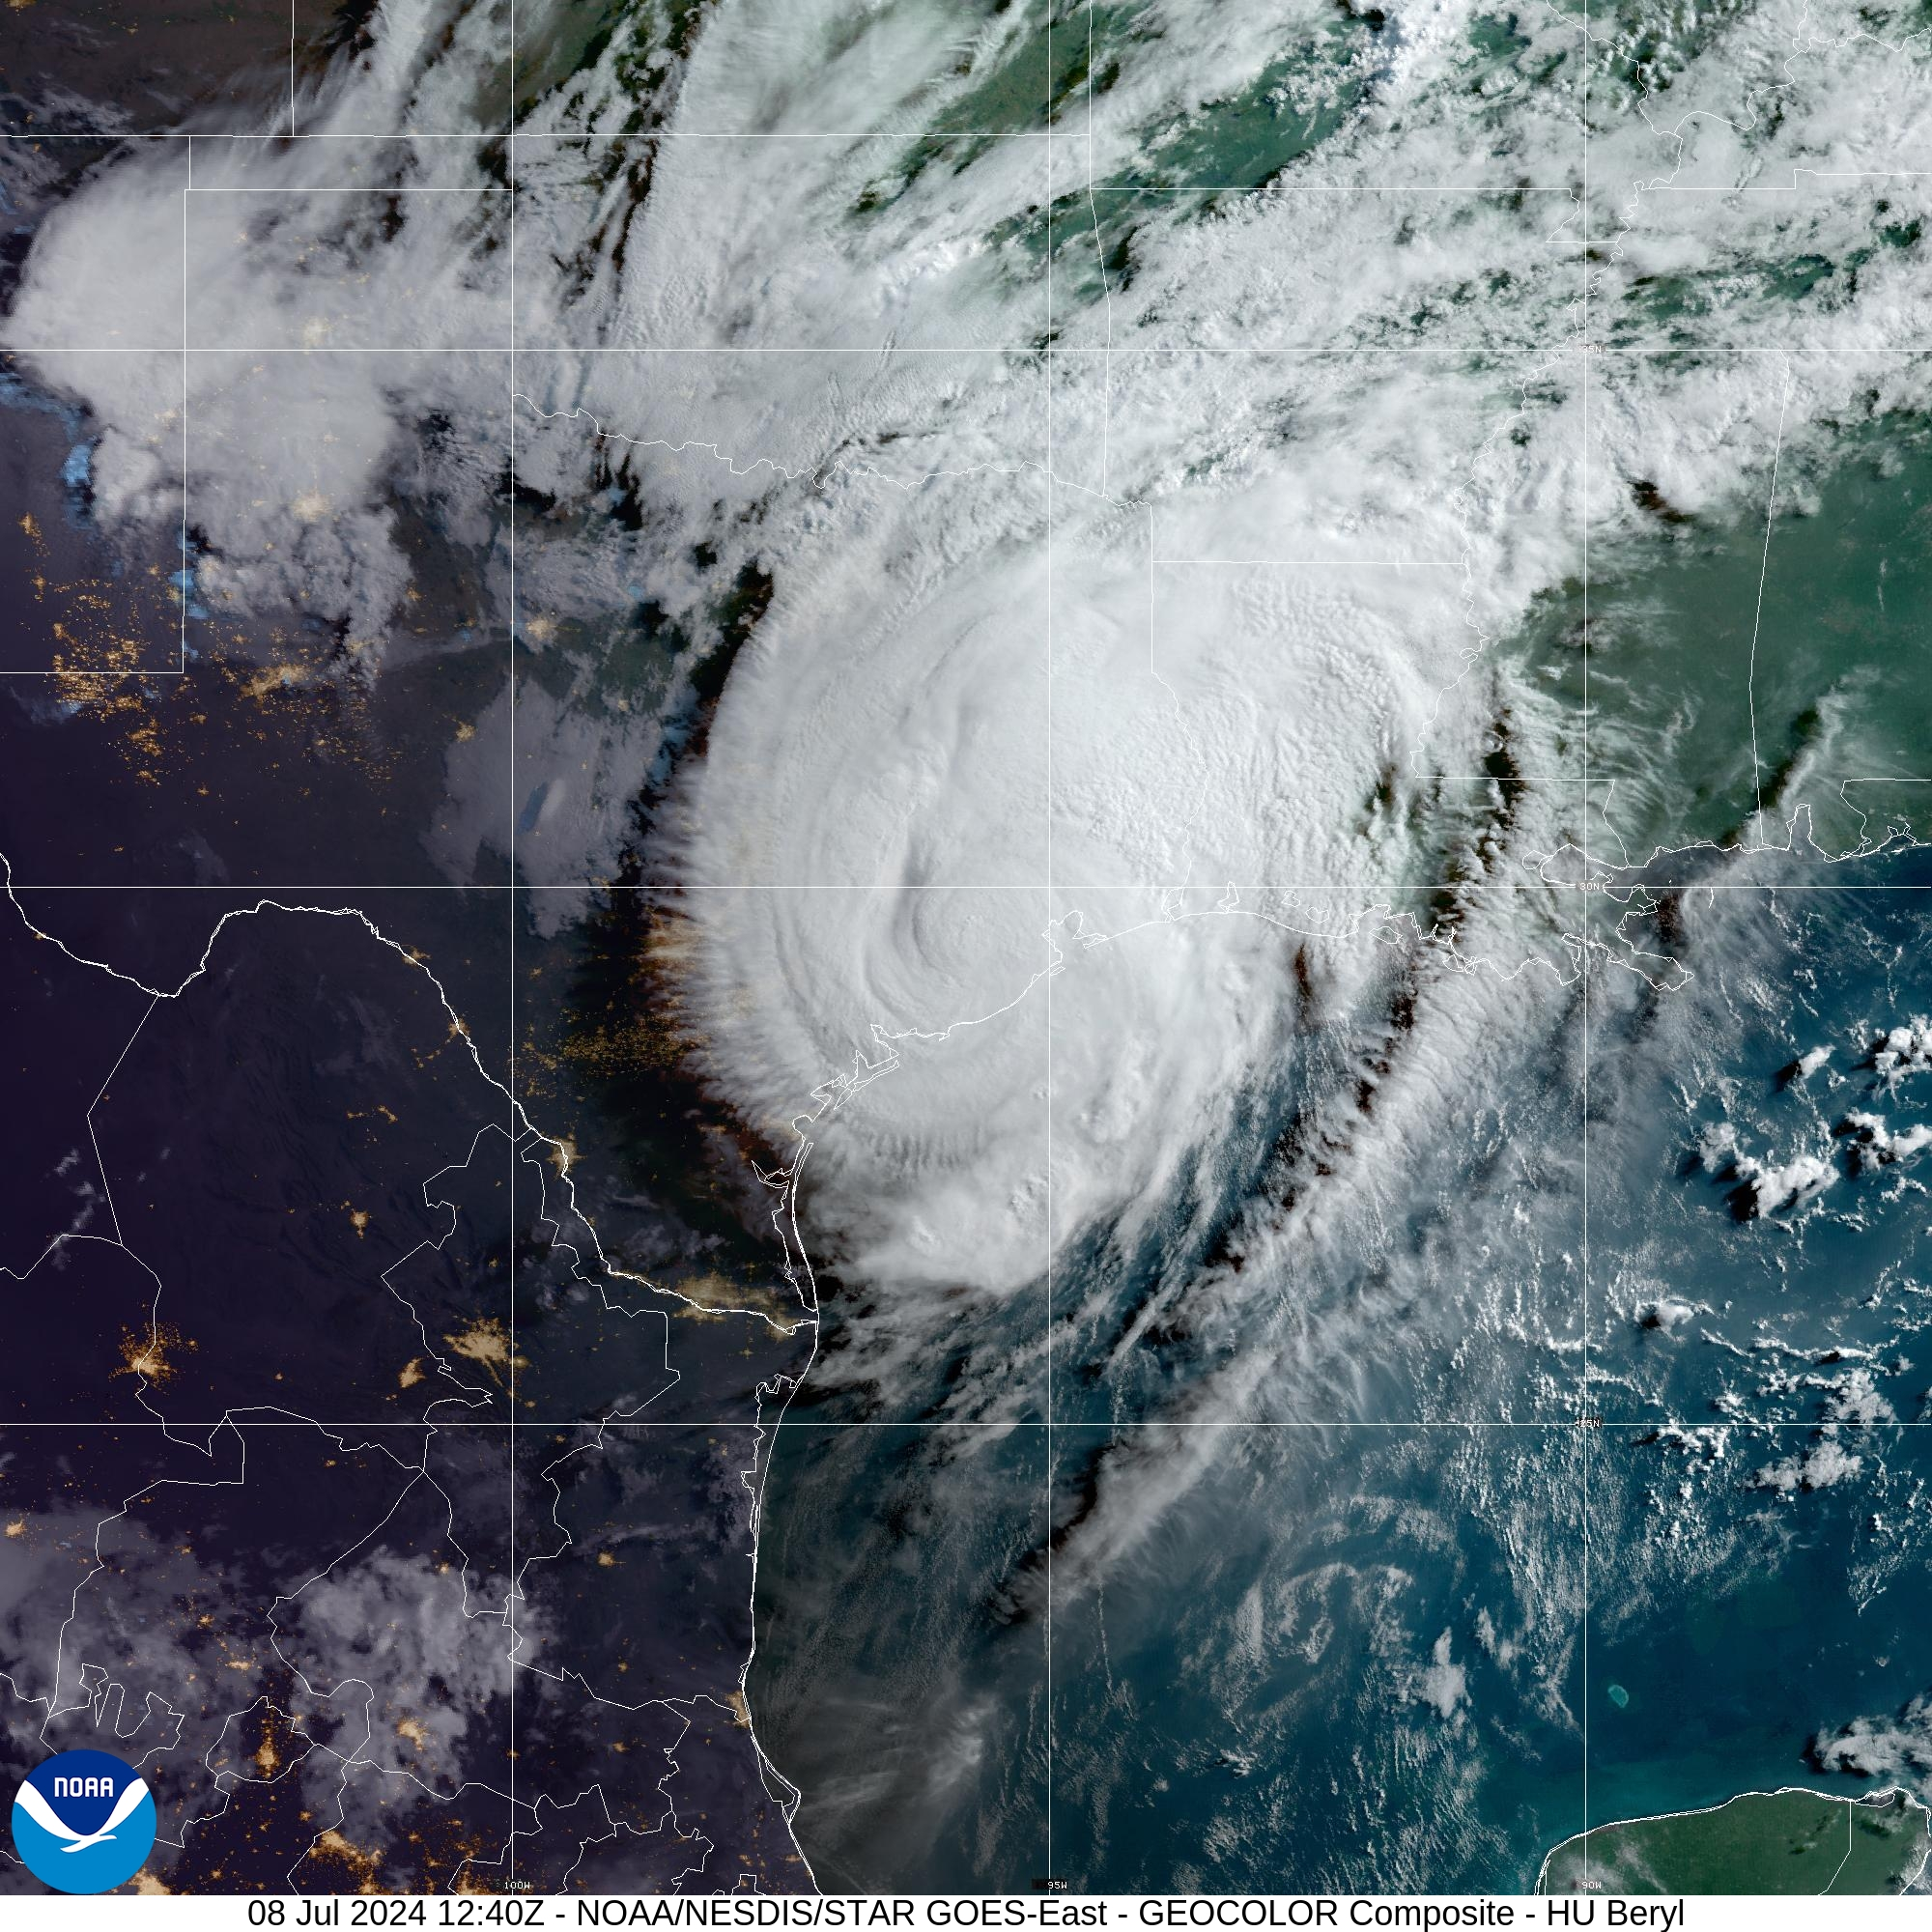
\includegraphics[width=0.6\textwidth]{docs/figuras/chapter5/20241901240_GOES16-ABI-FL-GEOCOLOR-AL022024-2000x2000.jpg}
	
	\centering
	Source: \url{https://www.star.nesdis.noaa.gov/star/index.php.}.
\end{figure}

Finally, the storm began to shift north-northeast, becoming a tropical storm by 10 AM CDT (15:00 UTC on July 8th). As it moved through the continental region, it weakened and transitioned to a tropical depression by 10 PM CDT (03:00 UTC on July 9th), just northwest of Shreveport, Louisiana.

Over the United States, the most intense rainfall occurred in the Houston metropolitan area in southeastern Texas, where widespread totals ranged from 8 to 12 inches, with local maxima of 14.99 inches in Thompsons and 14.88 inches at a HCFCD station in western Houston \cite{li2025generative}.

Based on this overview of the storm, Figure 4 has been created to illustrate the study area of interest, highlighting the significant landfalls made during its progression.

\begin{figure}[h!]
	\centering
	\caption{Spatial Domain of Hurricane Beryl's Development and Trajectory.}
	\label{fig:spatialdomainberyl}\includegraphics[width=\textwidth,height=\textheight,keepaspectratio]{docs/figuras/chapter5/map_with_cat_path.png}
	\centering
	Source: Made by the author (2025).
\end{figure}

The observational period for this study encompasses a six-day interval from 00 UTC on July 3 to 00 UTC on July 9, 2024, as illustrated by the gray bullet points in Figure \ref{fig:spatialdomainberyl}. Notably, this analysis will focus on a post-Category 5 storm. Whereas the system was active from June 28 to July 9, our analysis concentrates primarily on this specific timeframe. A sensitivity analysis regarding an earlier forecast of the observation period will be conducted and discussed in subsequent sections. This study encompasses significant geographical features, including the passage through Jamaica, which recorded the highest levels of rainfall in the Caribbean, the Yucatan landfall as denoted by the square E in Figure \ref{fig:spatialdomainberyl}, and the subsequent landfall in Texas, indicated by the square F in Figure \ref{fig:spatialdomainberyl}.

% ======================================================================================= %

\section{Results and analysis of hurricane Beryl}

In this section, we will present the results in alignment with the established workflow and engage in a discussion regarding the questions outlined in Table \ref{tab:questions}. The subsequent subsections will detail the trajectory, intensity, and rainfall analyses. To conclude, we will provide a summary discussion highlighting the key outcomes of the model and evaluating the overall performance of MONAN in comparison with ERA5 reanalysis.

By the workflow sequence, we will begin by addressing the selection process. Table~\ref{tab:experiments_long} illustrates all the experiments that were conducted.

\begin{table}[H]
	\centering
	\caption{All performed experiments}
	\label{tab:experiments_long}
	\renewcommand{\arraystretch}{1.2}
	\resizebox{\textwidth}{!}{
		\begin{tabular}{
				>{\centering\arraybackslash}m{3.5cm}
				>{\centering\arraybackslash}m{9cm}
				>{\centering\arraybackslash}m{4cm}
			}
			\toprule
			\textbf{Experiment} & \textbf{Description} & \textbf{ID} \\
			\midrule
			
			Cold Pool Effect 
			& Turn on and off the cold pool parameterization scheme 
			& \makecell[l]{CP-ON\\CP-OFF (Control)} \\
			\midrule
			
			Initial Condition Day 
			& Compares the effect of two initial conditions, June 29, July 2nd (noon), and July 3rd. Tested with 1st July 
			& \makecell[l]{CP-29\\CP-01\\CP-02T12\\CP-03} \\
			\midrule
			
			Cold Pool Lifetime 
			& Compares the effect of cold pool life time being 1h, 2h (default), 3h, and 6h 
			& \makecell[l]{CP-1H\\CP-2H\\CP-3H\\CP-6H} \\
			\midrule
			
			Maximum Downdraft Height 
			& Compares the effect of the maximum downdraft height, being 0.25, 0.35, and 0.50 
			& \makecell[l]{CP-D025\\CP-D035\\CP-D050} \\
			\midrule
			
			Resolution Experiment 
			& Evaluate the resolution effect on the results, degrading it into 60 km and enhancing it into 15 km 
			& \makecell[l]{CP-15km\\CP-30km (Control)\\CP-60km} \\
			\midrule
			
			Type of Initial Condition 
			& Changes the type of initial condition to be from the GFS model 
			& \makecell[l]{CP-ERA5 (Control) \\(CP-GFS)} \\
			\midrule
			
			Best Configuration Test 
			& A run with 2 changes inside the cold pool parameters 
			& \makecell[l]{CP-1HD050\\CP-1HD05015km} \\
			\bottomrule
		\end{tabular}
	}
	
	\vspace{2mm}
	{\centering Source: Made by the author (2025).\par}
\end{table}

The “ID” column serves as a reference for the names of the experiments. It is important to note that in the results, CP-ON represents the default configuration. In the sensitivity analyses conducted, the default values are specified in the labels. For instance, in the “Resolution Experiment,” the default configuration is set to a grid of 30 km (CP-30km), which is then changed to 60 km (CP-60km) and 15 km (CP-15km). To clarify, the following table emphasizes the default parameters:

\begin{table}[H]
	\centering
	\caption{Default values for the cold pool parameterization scheme}
	\label{tab:cp_def}
	\renewcommand{\arraystretch}{1.2}
	\resizebox{\textwidth}{!}{
		\begin{tabular}{
				>{\centering\arraybackslash}m{5.5cm} 
				>{\centering\arraybackslash}m{9cm}
			}
			\toprule
			\textbf{Parameter} & \textbf{Default value} \\
			\midrule
			Initial Condition Day & July 3rd, 2024 \\
			Cold Pool Lifetime & 2 h \\
			Maximum Downdraft Height & 0.35 \\
			Resolution Experiment & 30 km horizontal grid \\
			Type of initial condition & Coming from ERA5 \\
			\bottomrule
		\end{tabular}
	}
	
	\vspace{2mm}
	{\centering Source: Made by the author (2025).\par}
\end{table}




We investigate the impact of cold pools by enabling (CP-ON) and disabling (CP-OFF) the parameterization, with CP-OFF serving as the control experiment in this case. In the subsequent rows, we conducted a sensitivity analysis on the parameters within the parameterization. Now our control experiment is the CP-ON configuration, with the Table \ref{tab:cp_def} parameters. For the “Initial Condition Day” experiment, we varied the initial integration times: June 29 (00 UTC), 2024; July 1 (00 UTC), 2024; and July 2 (12 UTC), 2024 - comparing them with the default time. These periods were selected because they correspond to key moments in the storm’s evolution: shortly after HB was classified as a tropical storm, one day before it reached Category 5, and the day it reached Category 5, respectively.

The “Cold Pool Lifetime” was adjusted from the default to durations of 1 hour, 3 hours, and 6 hours. The height of the mass flux above the surface is described by a parabolic function, and the coefficient of this function can be manipulated to alter the maximum height, with lower (higher) values indicating proximity (distance) to the surface. The “Type of Initial Condition” was switched from ERA5 to GFS, both initialized on July 3 (00 UTC), 2024.

During the computation of the initial 13 experiments, we observed that setting the cold pool lifetime to 1 hour and adjusting the maximum downdraft height coefficient to 0.5 resulted in lower errors in the initial results. Consequently, we conducted the “Best Configuration Test” with these parameter adjustments and repeated this configuration at 15 km, bringing the total number of experiments to 15. The reference data here is the best track dataset, and hereafter this dataset will be referenced as “NOAA”. 

Keeping this in mind, Figure~\ref{fig:all_tracks_before} shows all the trajectories for the 15 experiments, plus ERA5 and the reference best-track dataset.

\begin{figure}[!htb]
    \centering
    \caption{Comparison of Storm Tracks Across All 15 Experiments} % Título acima da figura
    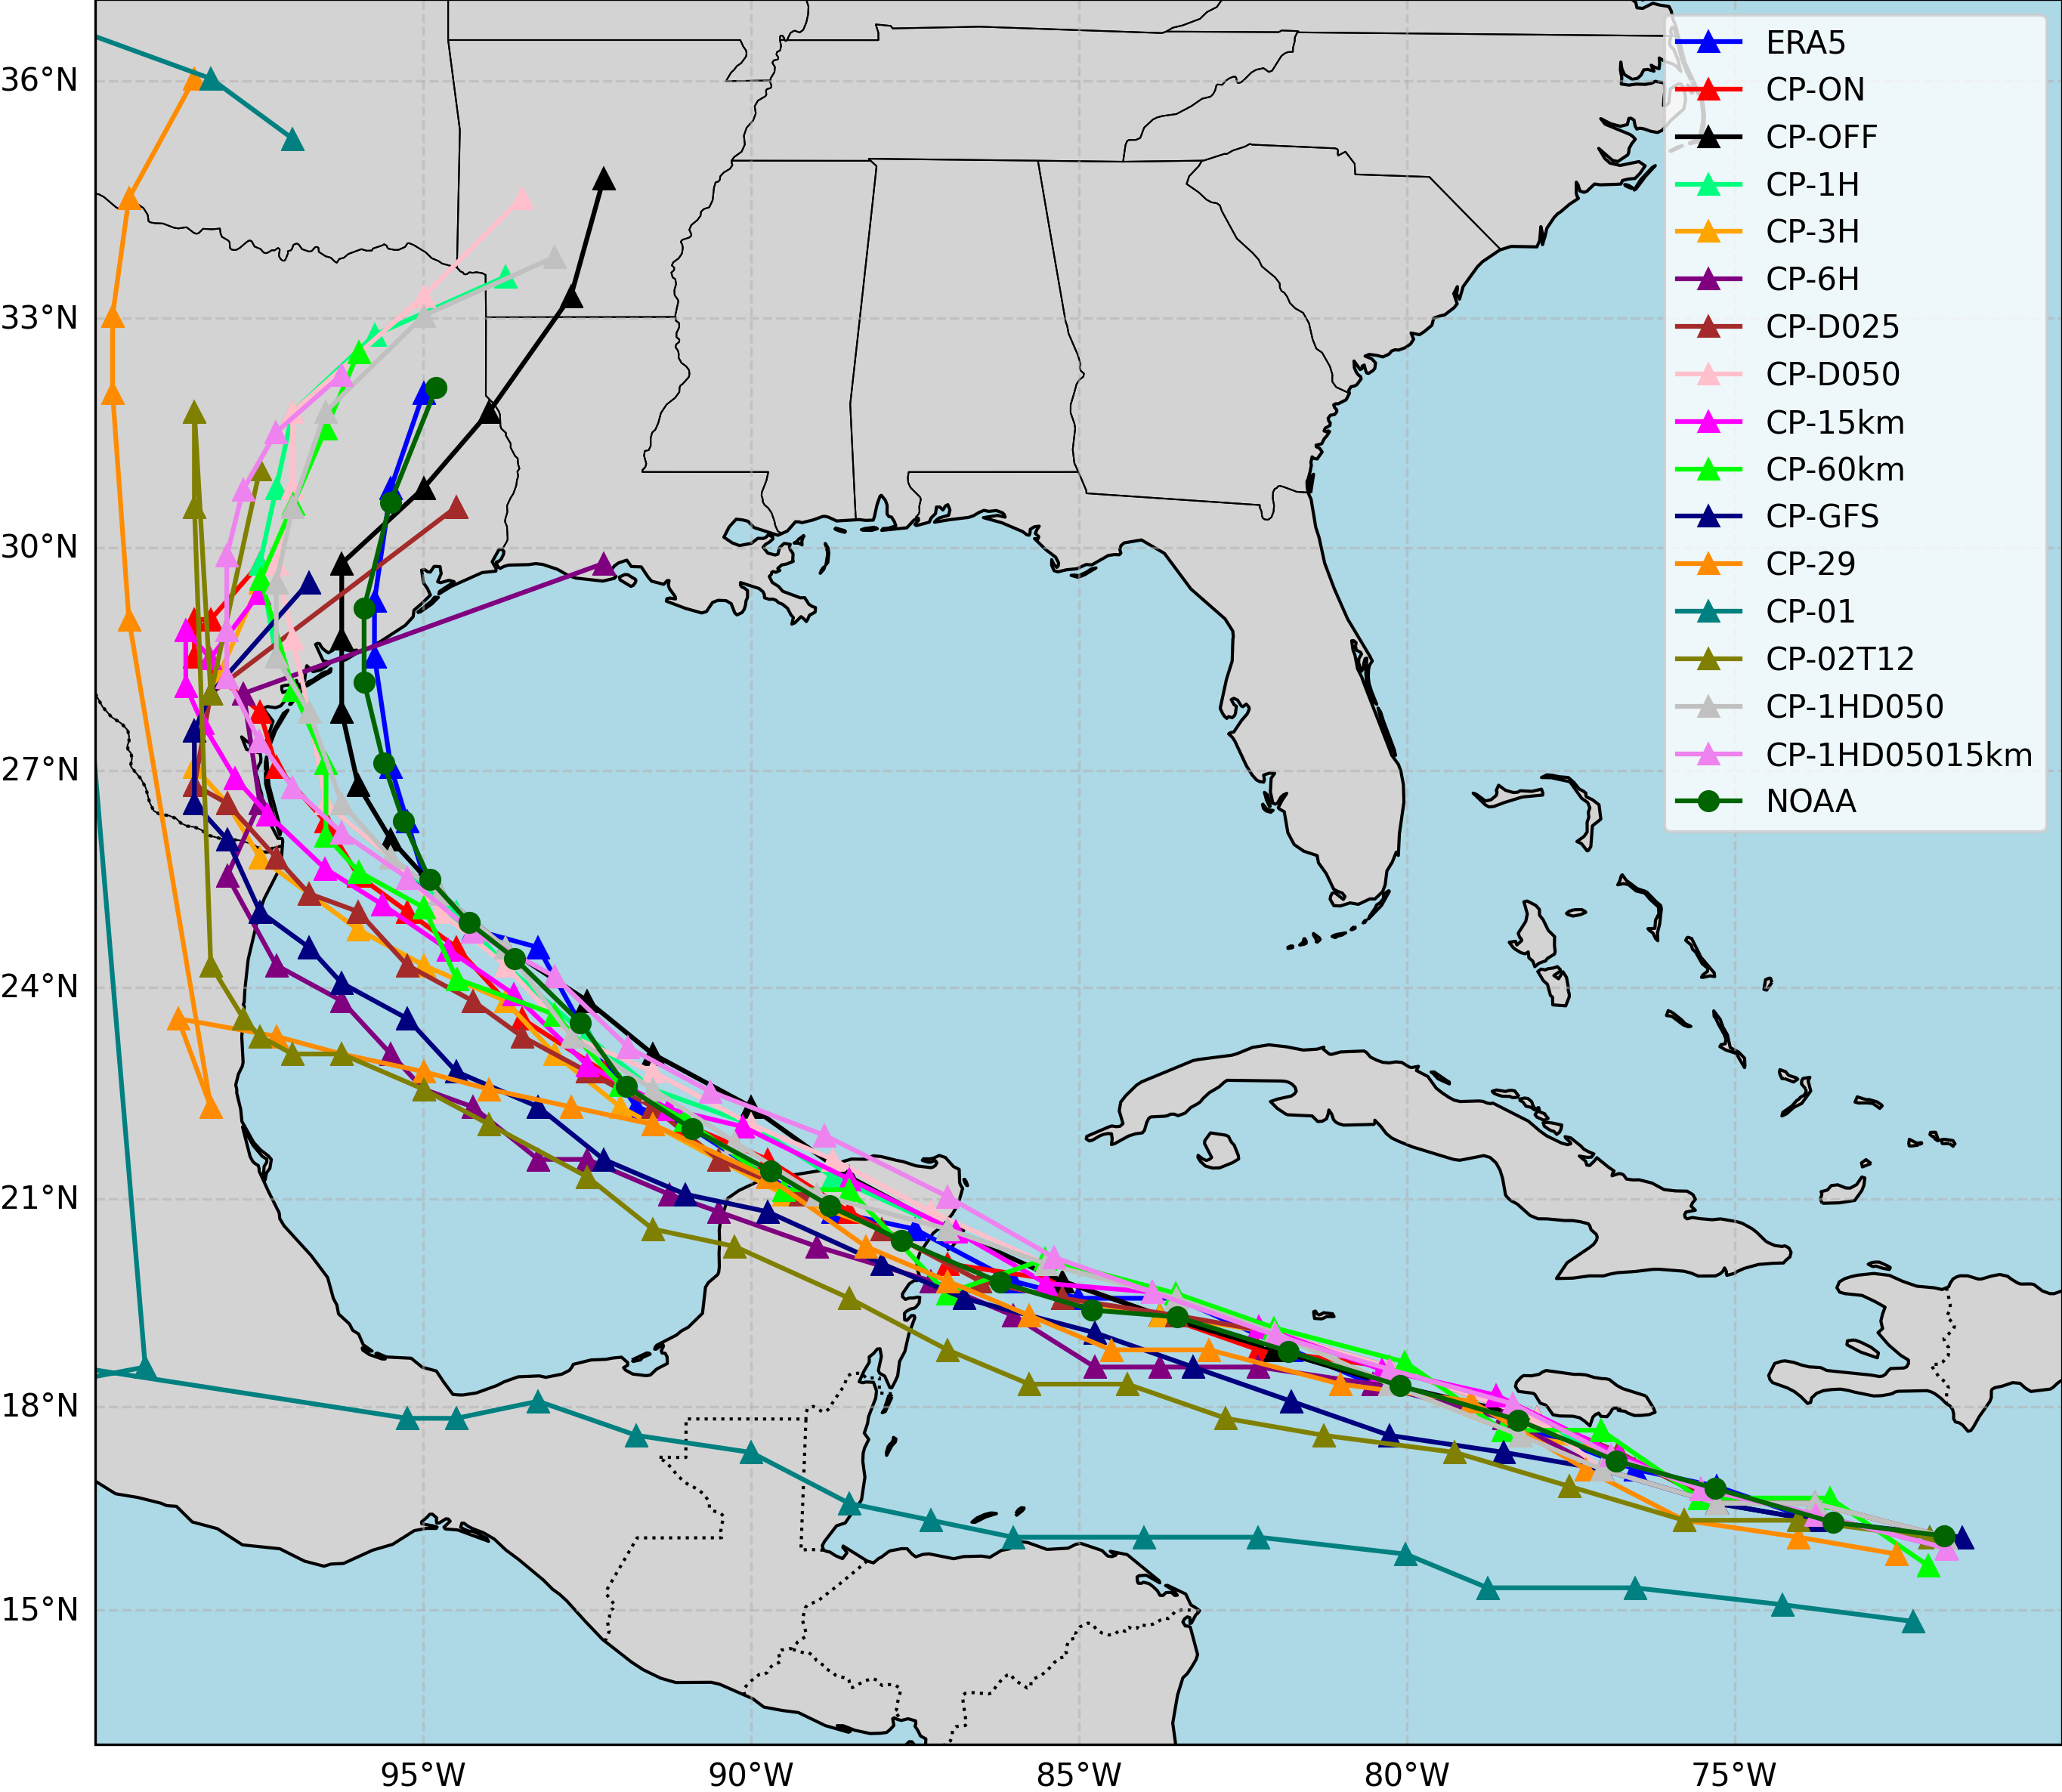
\includegraphics[width=\textwidth]{docs/figuras/chapter5/ALL_tracks_before_filter.png} % Substitua pelo caminho e extensão correta
    \vspace{0.5em}
    
    Source: Made by the author (2025). % Fonte abaixo da imagem
    \label{fig:all_tracks_before} % Label para referenciar no texto
\end{figure}

As one can see in Figure~\ref{fig:all_tracks_before}, the numerous experiments clutter the scene and make visual comparison difficult. But one could notice the deviation of CP-6H and CP-01, which could be candidates to be withdrawn. To better visualize the difference between the trajectories, the distance between each trajectory and the reference data (NOAA’s best track) was computed and shown in Figure~\ref{fig:panel_errors_before}.

\begin{figure}[!htb]
    \centering
    \caption{Errors (distance) between the trajectories} % Título acima da figura
    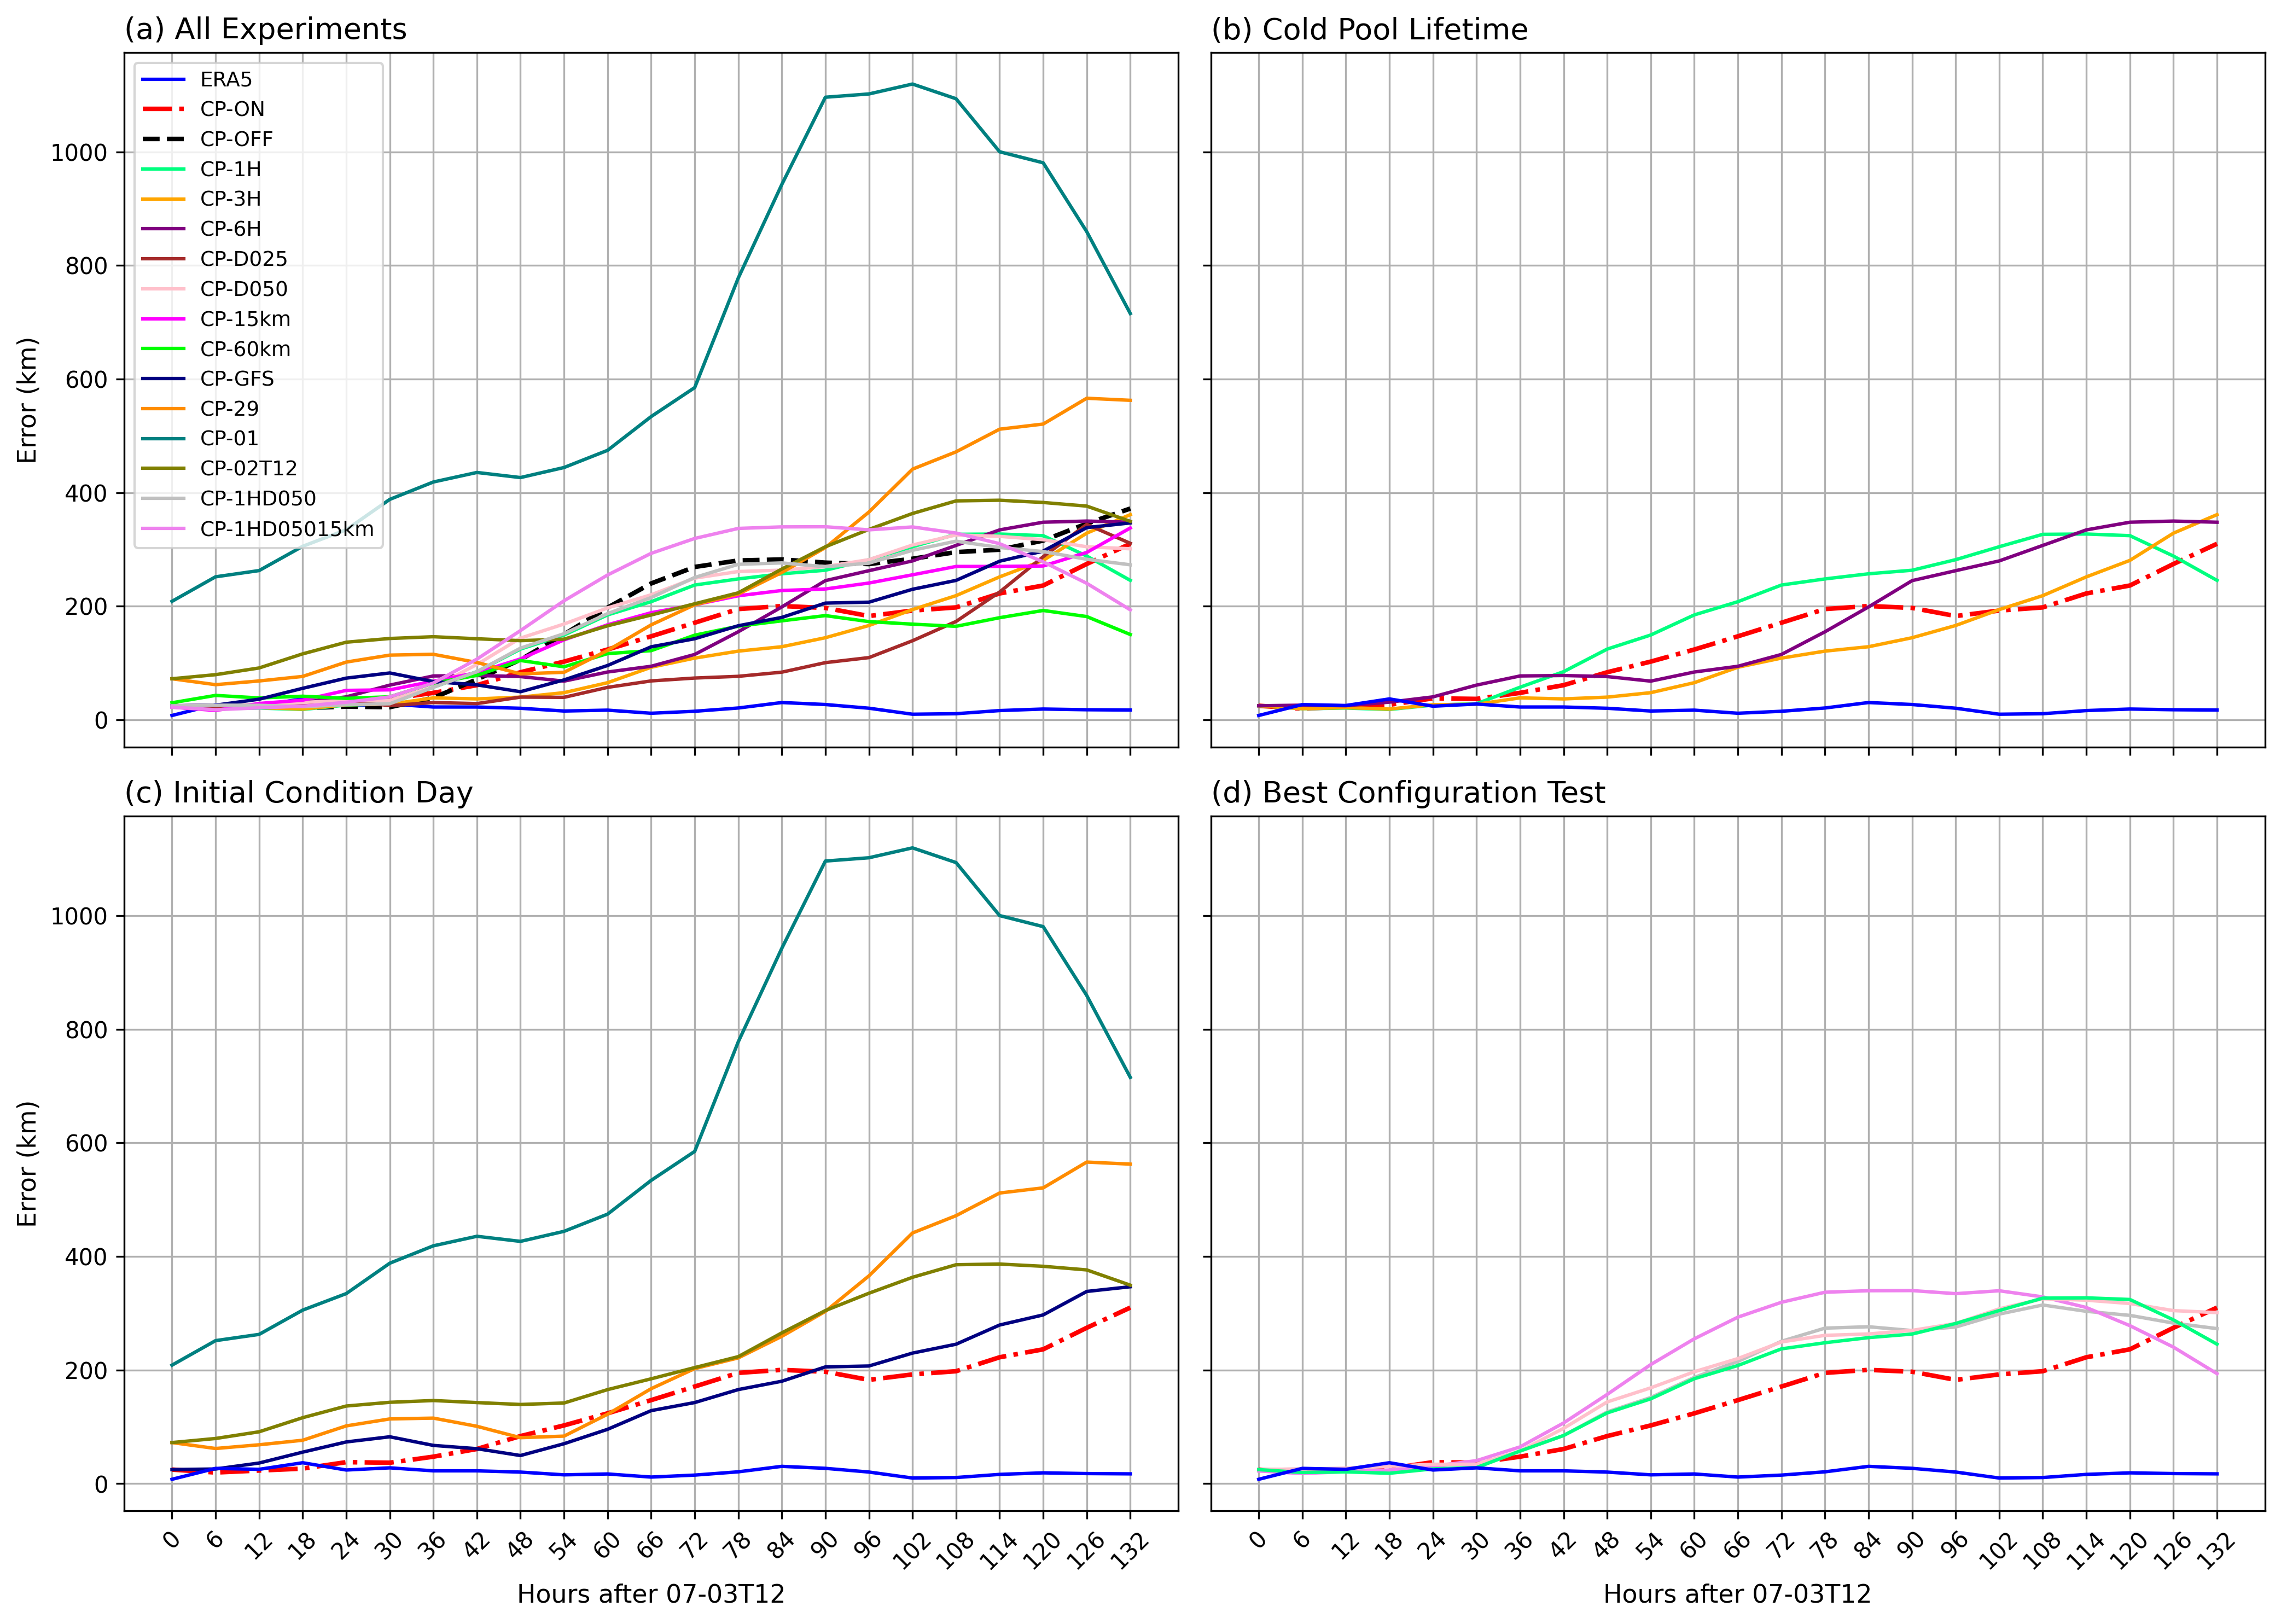
\includegraphics[width=\textwidth]{docs/figuras/chapter5/panel_2x2_error_comparison.png} % Substitua pelo caminho e extensão correta
    \vspace{0.5em}
    
    Source: Made by the author (2025). % Fonte abaixo da imagem
    \label{fig:panel_errors_before} % Label para referenciar no texto
\end{figure}

\pagebreak

It can be confirmed that CP-01 deviates significantly from the expected trajectory. Additionally, CP-6H offer limited discussion, as it is quite similar to the other experiments within their group. In Figure~\ref{fig:panel_errors_before} (d), CP-1HD05015km does not show a significant improvement and will consequently be withdrawn. We will retain CP-1HD050 to seek the effects related to this configuration in the context of other aspects of tropical cyclones.

To summarize the experiments we intend to keep, a new table has been created, similar to Table~\ref{tab:experiments_long}.

\pagebreak

\begin{table}[H]
	\centering
	\caption{Selected experiments}
	\label{tab:selected_experiments}
	\renewcommand{\arraystretch}{1.2}
	\resizebox{\textwidth}{!}{
		\begin{tabular}{
				>{\centering\arraybackslash}m{4cm}
				>{\centering\arraybackslash}m{9cm}
				>{\centering\arraybackslash}m{4cm}
			}
			\toprule
			Parameter & Description & ID \\
			\midrule
			
			Cold Pool Effect 
			& Turn on and off the cold pool parameterization scheme 
			& \makecell[l]{CP-ON\\CP-OFF (Control)} \\
			\midrule
			
			Initial Condition 
			& Compares the effect of two initial conditions, June 29, July 2nd (noon), and July 3rd. Tested with 1st July 
			& \makecell[l]{CP-29\\CP-02T12\\CP-03 (Control)} \\
			\midrule
			
			Cold Pool Lifetime 
			& Compares the effect of cold pool life time being 1h, 2h (default), 3h, and 6h 
			& \makecell[l]{CP-1H\\CP-2H (Control)\\CP-3H} \\
			\midrule
			
			Maximum Downdraft Height 
			& Compares the effect of the maximum downdraft height, being 0.25, 0.35, and 0.50 
			& \makecell[l]{CP-D025\\CP-D035 (Control)\\CP-D050} \\
			\midrule
			
			Resolution Experiment 
			& Evaluate the resolution effect on the results, degrading it into 60 km and enhancing it into 15 km 
			& \makecell[l]{CP-15km\\CP-30km (Control)\\CP-60km} \\
			\midrule
			
			Type of Initial Condition 
			& Changes the type of initial condition to be from the GFS model 
			& \makecell[l]{CP-ERA5 (Control)\\(CP-GFS)} \\
			\midrule
			
			Best Configuration Test 
			& A run with 2 changes inside the cold pool parameters 
			& CP-1HD050 \\
			\bottomrule
		\end{tabular}
	}
	
	\vspace{2mm}
	{\centering Source: Made by the author (2025).\par}
\end{table}


In the following subsection we will continue the results now keeping in mind the experiments listed at Table~\ref{tab:selected_experiments}.

%%%%%%%%%%%%%%%%%%%%%%%%%%%%%%%%%%%%%%%%%%

\subsection{Trajectory}


All trajectories are displayed in the Figure~\ref{fig:all_tracks_selected}. The trajectories of each group of the Table~\ref{tab:selected_experiments} can be found at Appendix B.

\begin{figure}[!ht]
    \centering
    \caption{All tracks with selected experiments from Table~\ref{tab:selected_experiments}} % Título acima da figura
    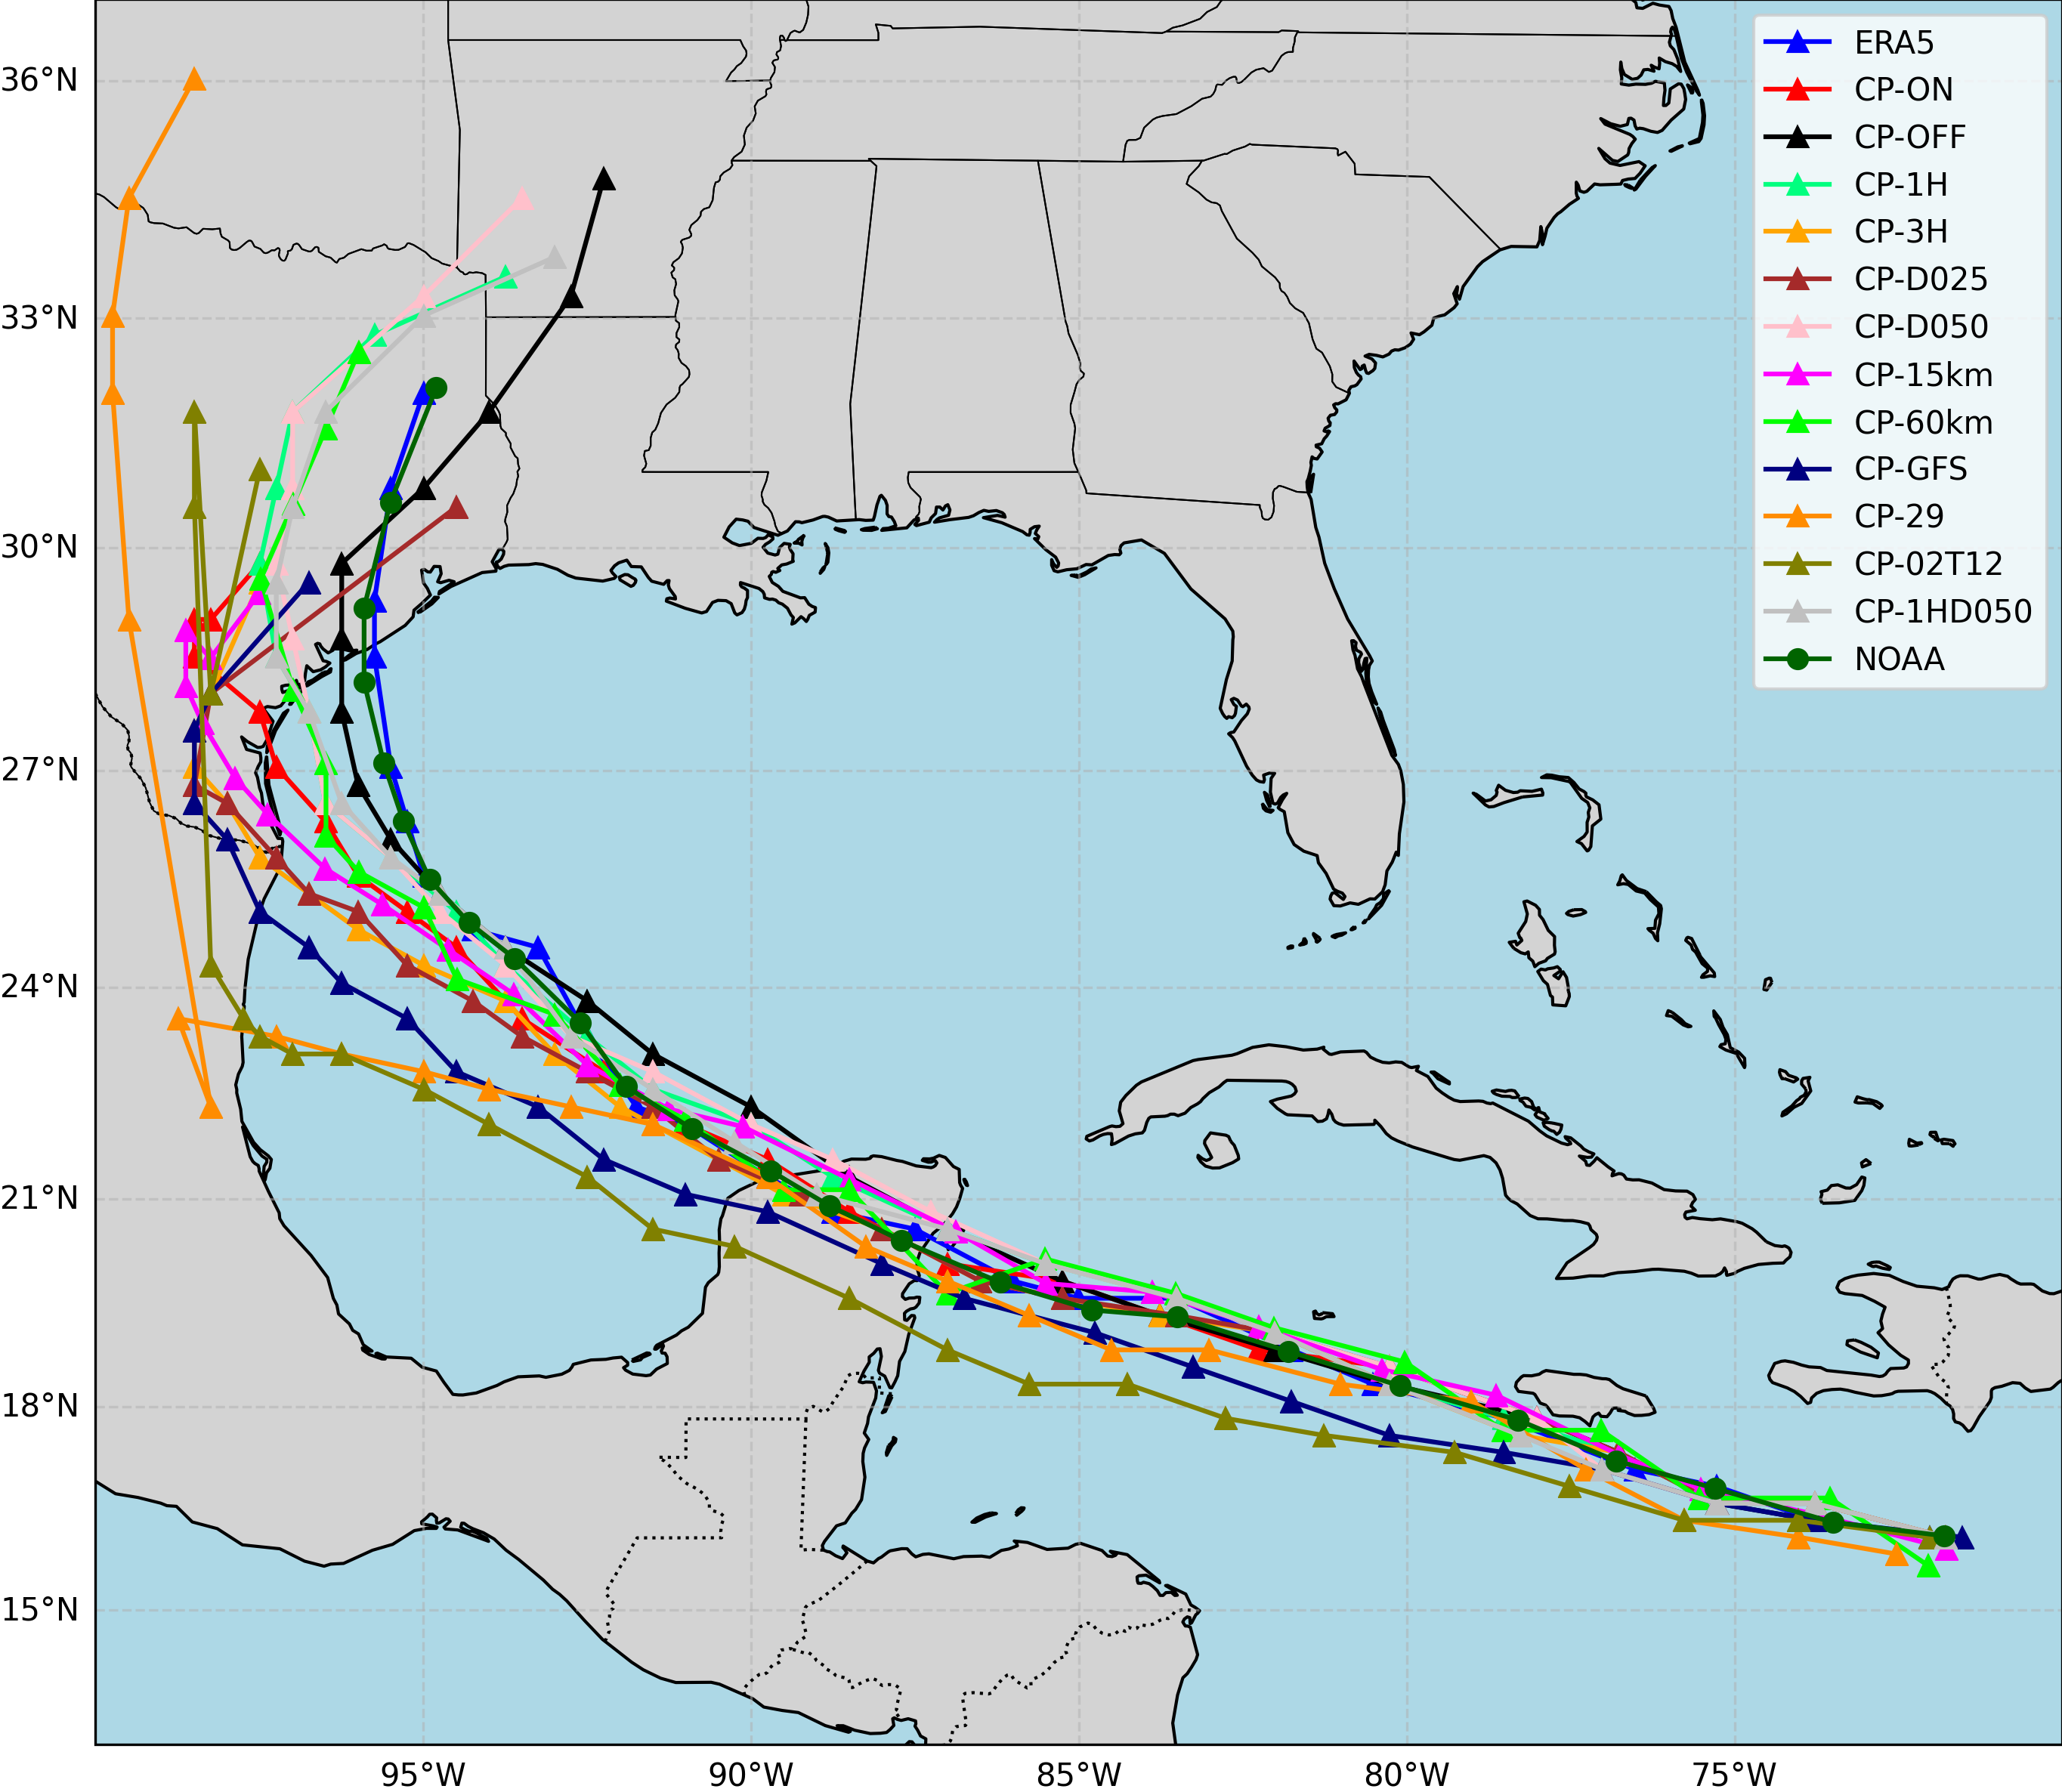
\includegraphics[width=\textwidth]{docs/figuras/chapter5/ALL_tracks_filter.png} 
    \vspace{0.5em}
    
    Source: Made by the author (2025). % Fonte abaixo da imagem
    \label{fig:all_tracks_selected} % Label para referenciar no texto
\end{figure}

This figure presents a map generated utilizing a tracking algorithm developed by the author. Firstly, the algorithm extracts each point corresponding to the minimum central pressure from the best track data between July 3rd and July 9th, 2024, sweeping a total integration period of 144 hours, with data plotted at 6-hour intervals. Furthermore, the minimum Mean Sea Level Pressure (MSLP) of the MONAN’s forecast and ERA5 reanalysis is extracted within a predefined spatial box surrounding the best track minimum central pressure. For instance, the initial bullet point depicted in dark green (representing NOAA’s best track at approximately 72.5° W) corresponds to the minimum central pressure obtained with the best track on July 3rd (00 UTC), 2024, while the final bullet point in dark green represents the data from July 9th (00 UTC), 2024 (close to 95° W).

At first glance, the reader will notice the observed congruence between the ERA5 reanalysis data and the best track observations. This strong agreement may be attributable to the reanalysis nature (Dulac et al., 2023), which integrates observational datasets throughout the integration period, thereby leading to this expected behaviour.

The CP-ON and CP-OFF experimental configurations exhibit comparable results for the majority of the integration period, with pronounced discrepancies evident near the Texas landfall and around the Yucatán Peninsula. A more detailed examination of these differences is warranted with other metrics. Concerning the cold pool lifetime, a 3-hour interval significantly deteriorates the accuracy of the forecasts. Furthermore, the downdraft maximum height coefficient of 0.50 appears to yield less precise results relative to the default values of 0.35 and 0.25. The trajectory forecasts utilizing a 60 km horizontal resolution demonstrate closer alignment with the reference data, outperforming the 15 km and 30 km horizontal resolutions, with the 60 km configuration exhibiting superior performance. Additionally, forecasts initialized with the GFS (CP-GFS) model appear to underperform in comparison to those initialized with ERA5.

It is observed that when initialization occurs before July 3rd (00 UTC), 2024, a visible degradation in trajectory forecast accuracy ensues. Note that there is a tendency for earlier initialization to result in poorer forecasts, a fact that can be confirmed later on with the MAE and RMSE metrics. This underscores the necessity of incorporating a module within the model to assess ensembles of initial conditions, also in agreement with what is found in the literature \cite{donkin2023capability}.

Finally, the configuration incorporating two parameters that have been changed simultaneously does not reveal significant deviations from the default setup. Overall, the forecasts exhibit a westward bias, a phenomenon that is also apparent in forecasts issued by the Hurricane Analysis and Forecast System (HAFS), as shown at Figure \ref{fig:berryl3rd}.

\begin{figure}[!ht]
	\centering
	\caption{Forecast made for Hurricane Beryl starting at July 3rd (00 UTC), 2024, available at the HAFS website} % Título acima da figura
	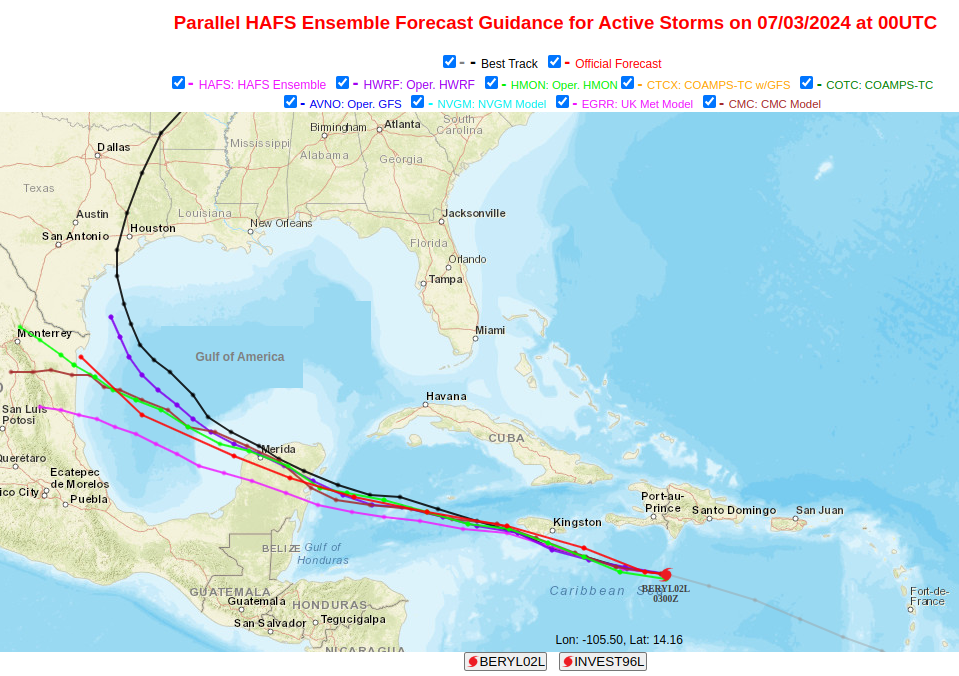
\includegraphics[width=\textwidth]{docs/figuras/chapter5/HAFS_trajectory.png} 
	\vspace{0.5em}
	Source: \url{https://www.emc.ncep.noaa.gov/HAFS/HAFSEPS/index.php} . % Fonte abaixo da imagem
	\label{fig:berryl3rd} % Label para referenciar no texto
\end{figure}

The next panel provides complementary information to the analysis, now in a more quantitative manner. It is important to mention that the time series display the errors after 12h of spin-up, and that value is maintained and the further analysis. In Figure (a), it is possible to better distinguish the differences among the experiments over time. In other words, it shows when each experiment presents lower errors throughout the integration period, along with an initial comparison among them. It is important to note that the vertical line E indicates the moment the hurricane makes landfall on the Yucatan Peninsula, while the vertical line F marks its entry into Texas. In Figure (b), this comparison becomes even clearer, especially because the bars are arranged vertically from the lowest to the highest error (from top to bottom).

\begin{figure}[!ht]
	\centering
	\caption{Track errors of the MONAN forecast and ERA5 reanalysis with the best track as reference. 12 hours of model spin-up are withdrawn from the analysis. (a) is displayed the distance error computed as the great circle, and (b), the MAE and RMSE calculated from (a).} % Título acima da figura
	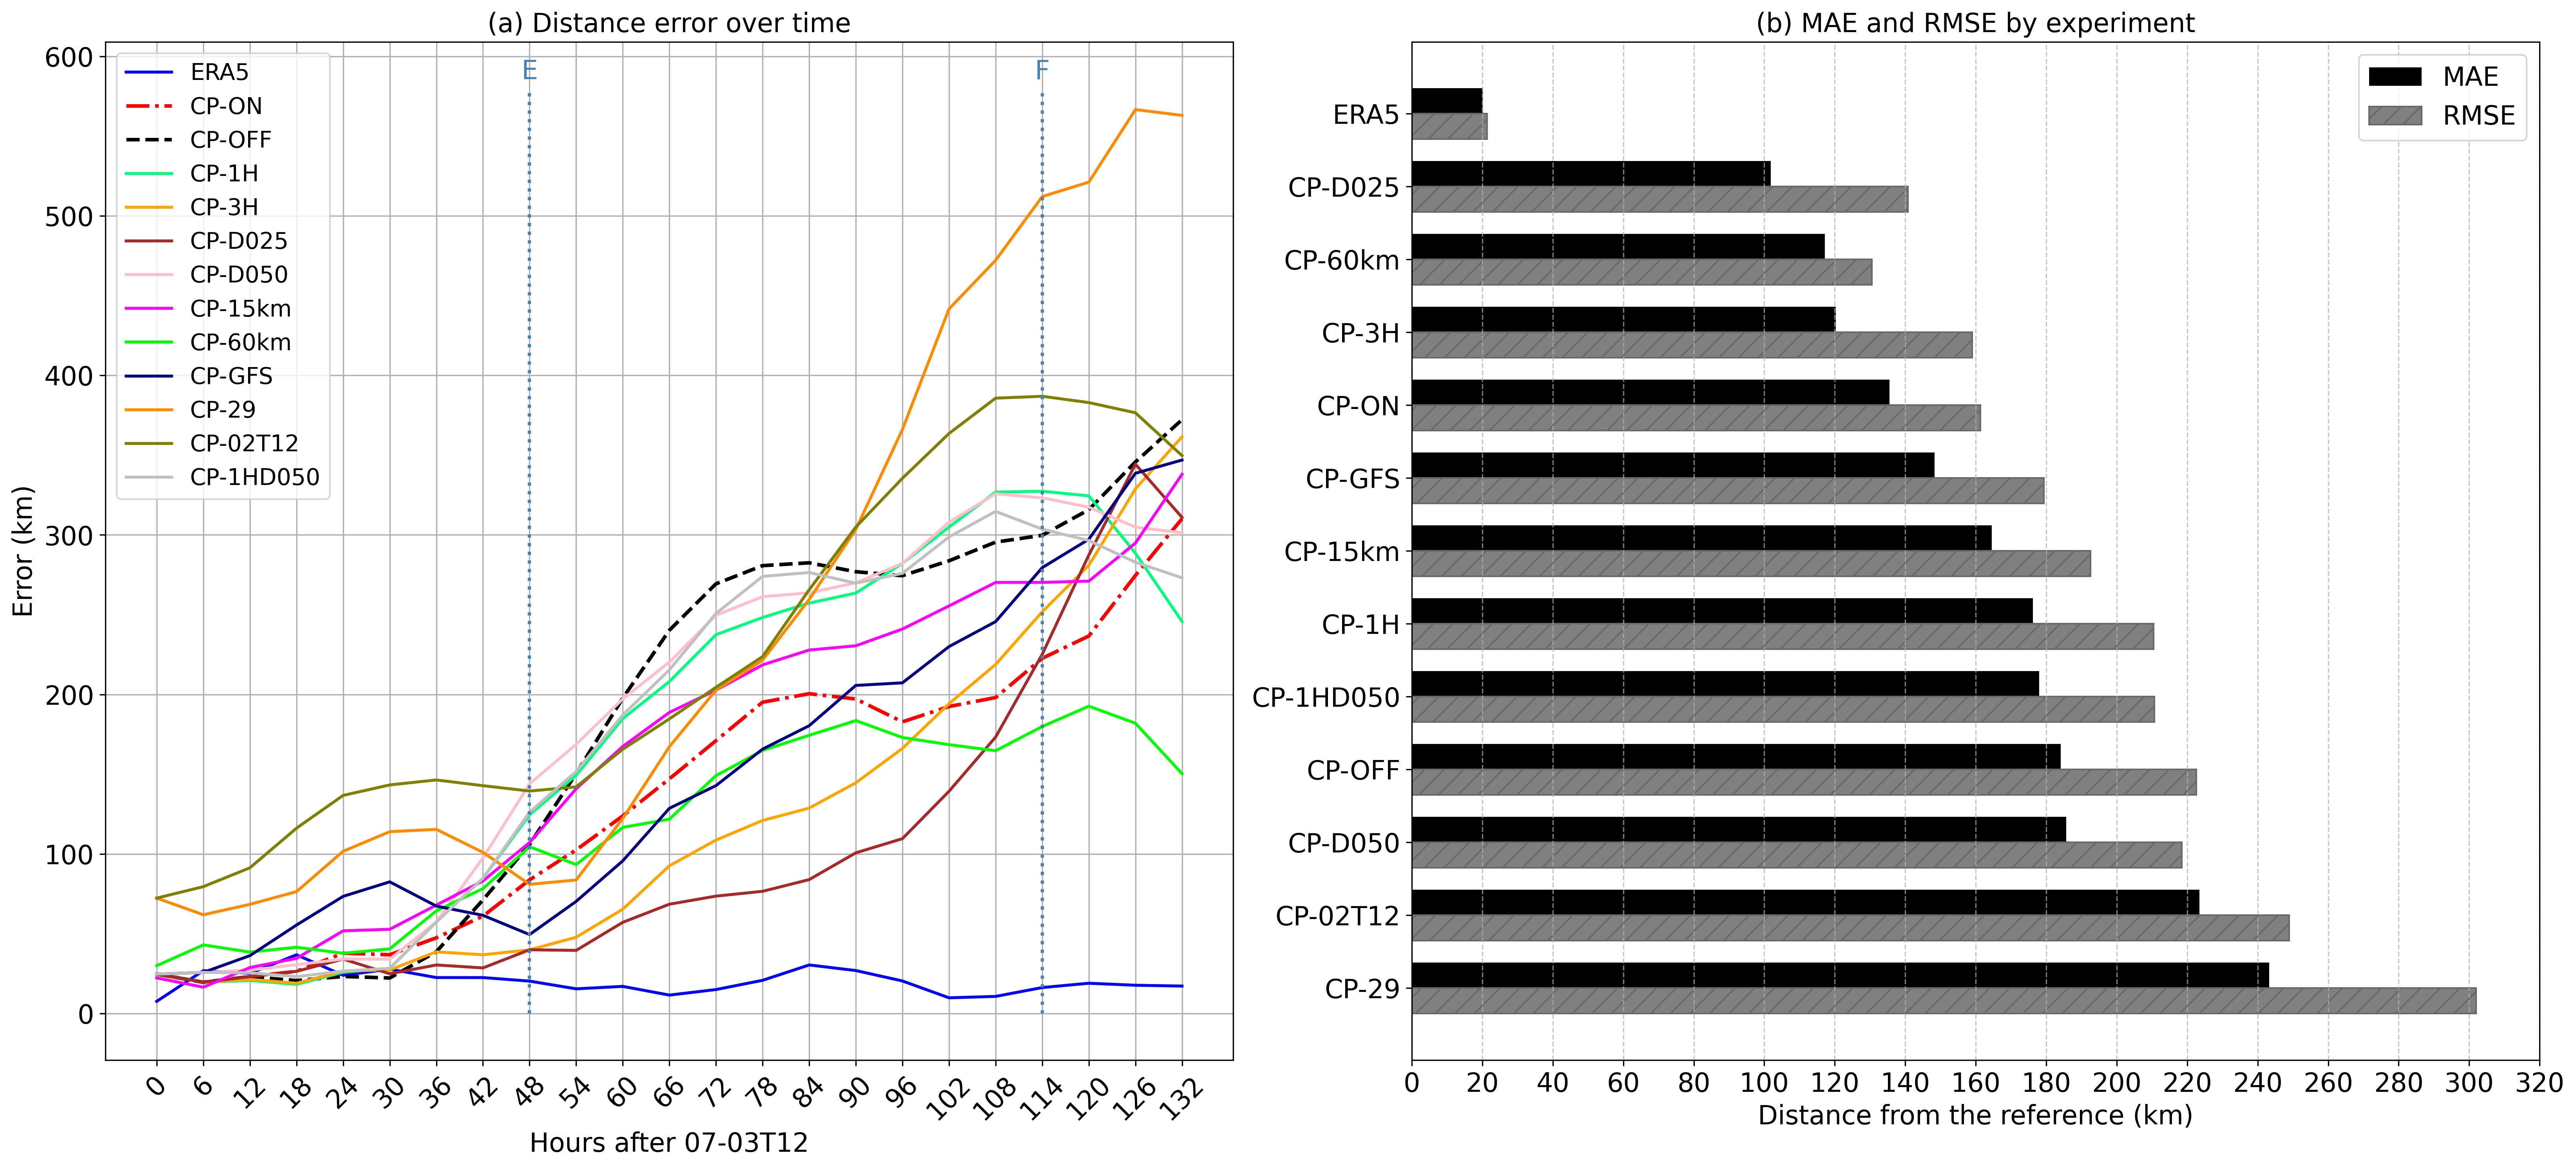
\includegraphics[width=\textwidth]{docs/figuras/chapter5/panel_errors_mae_rmse_FINAL.png} 
	\vspace{0.5em}
	Source: Made by the author, (2025).  % Fonte abaixo da imagem
	\label{fig:trackerrors} % Label para referenciar no texto
\end{figure}

As shown in the previous figure, ERA5 delivers the best track prediction performance. This could be attributed to the fact that ERA5 is a reanalysis product, meaning that observational data assimilation is injected into the model at each integration step. A fairer comparison would require conducting this analysis with another model similar to MONAN, which will be left for future work.

Overall, forecasts tend to show errors below 100 km up to 42 hours of lead time, except for those initialized earlier (CP-29 and CP-02T12). After 60 hours of forecast (two and a half days), some experiments begin to exceed 200 km of error. However, cold pool influence on track prediction only reaches this threshold after 84 hours (three and a half days), and the CP-D025 experiment only reaches it after about 111 hours (four and a half days). Therefore, we observe that with cold pool parameterization, forecast skill is extended by up to two days compared to the configuration without this scheme, for this specific case study.

In the literature, the best forecast limit reported is around 120 hours (five days) \cite{zhou2020prospects}, \cite{sippel2022impacts}. It is worth emphasizing that forecast errors beyond this threshold should be considered “chaotic,” given the nonlinear nature of the system.

The computation of MAE and RMSE provides insights into the overall error behavior in track forecasts. While MAE offers a generalized view of the error, RMSE takes into account the squared deviations, assigning more weight to larger errors at each time step. In general, it is notable that simply enabling the cold pool parameterization (CP-ON) already improved the track forecast, reducing the MAE by approximately 22\% compared to CP-OFF. Furthermore, we observe that tuning the parameters, such as in CP-D025, CP-3H, and modifying the resolution to 60 km (CP-60km), further enhanced this performance.

By observing the Figure \ref{fig:berryl3rd} and Figure \ref{fig:trackerrors}, one could notice the westward deviation in the forecast. The next panel showing the CTE and ATE can confirm this behaviour, at Figure \ref{fig:cte}.

\begin{figure}[!ht]
	\centering
	\caption{CTE (a) and ATE (b).} % Título acima da figura
	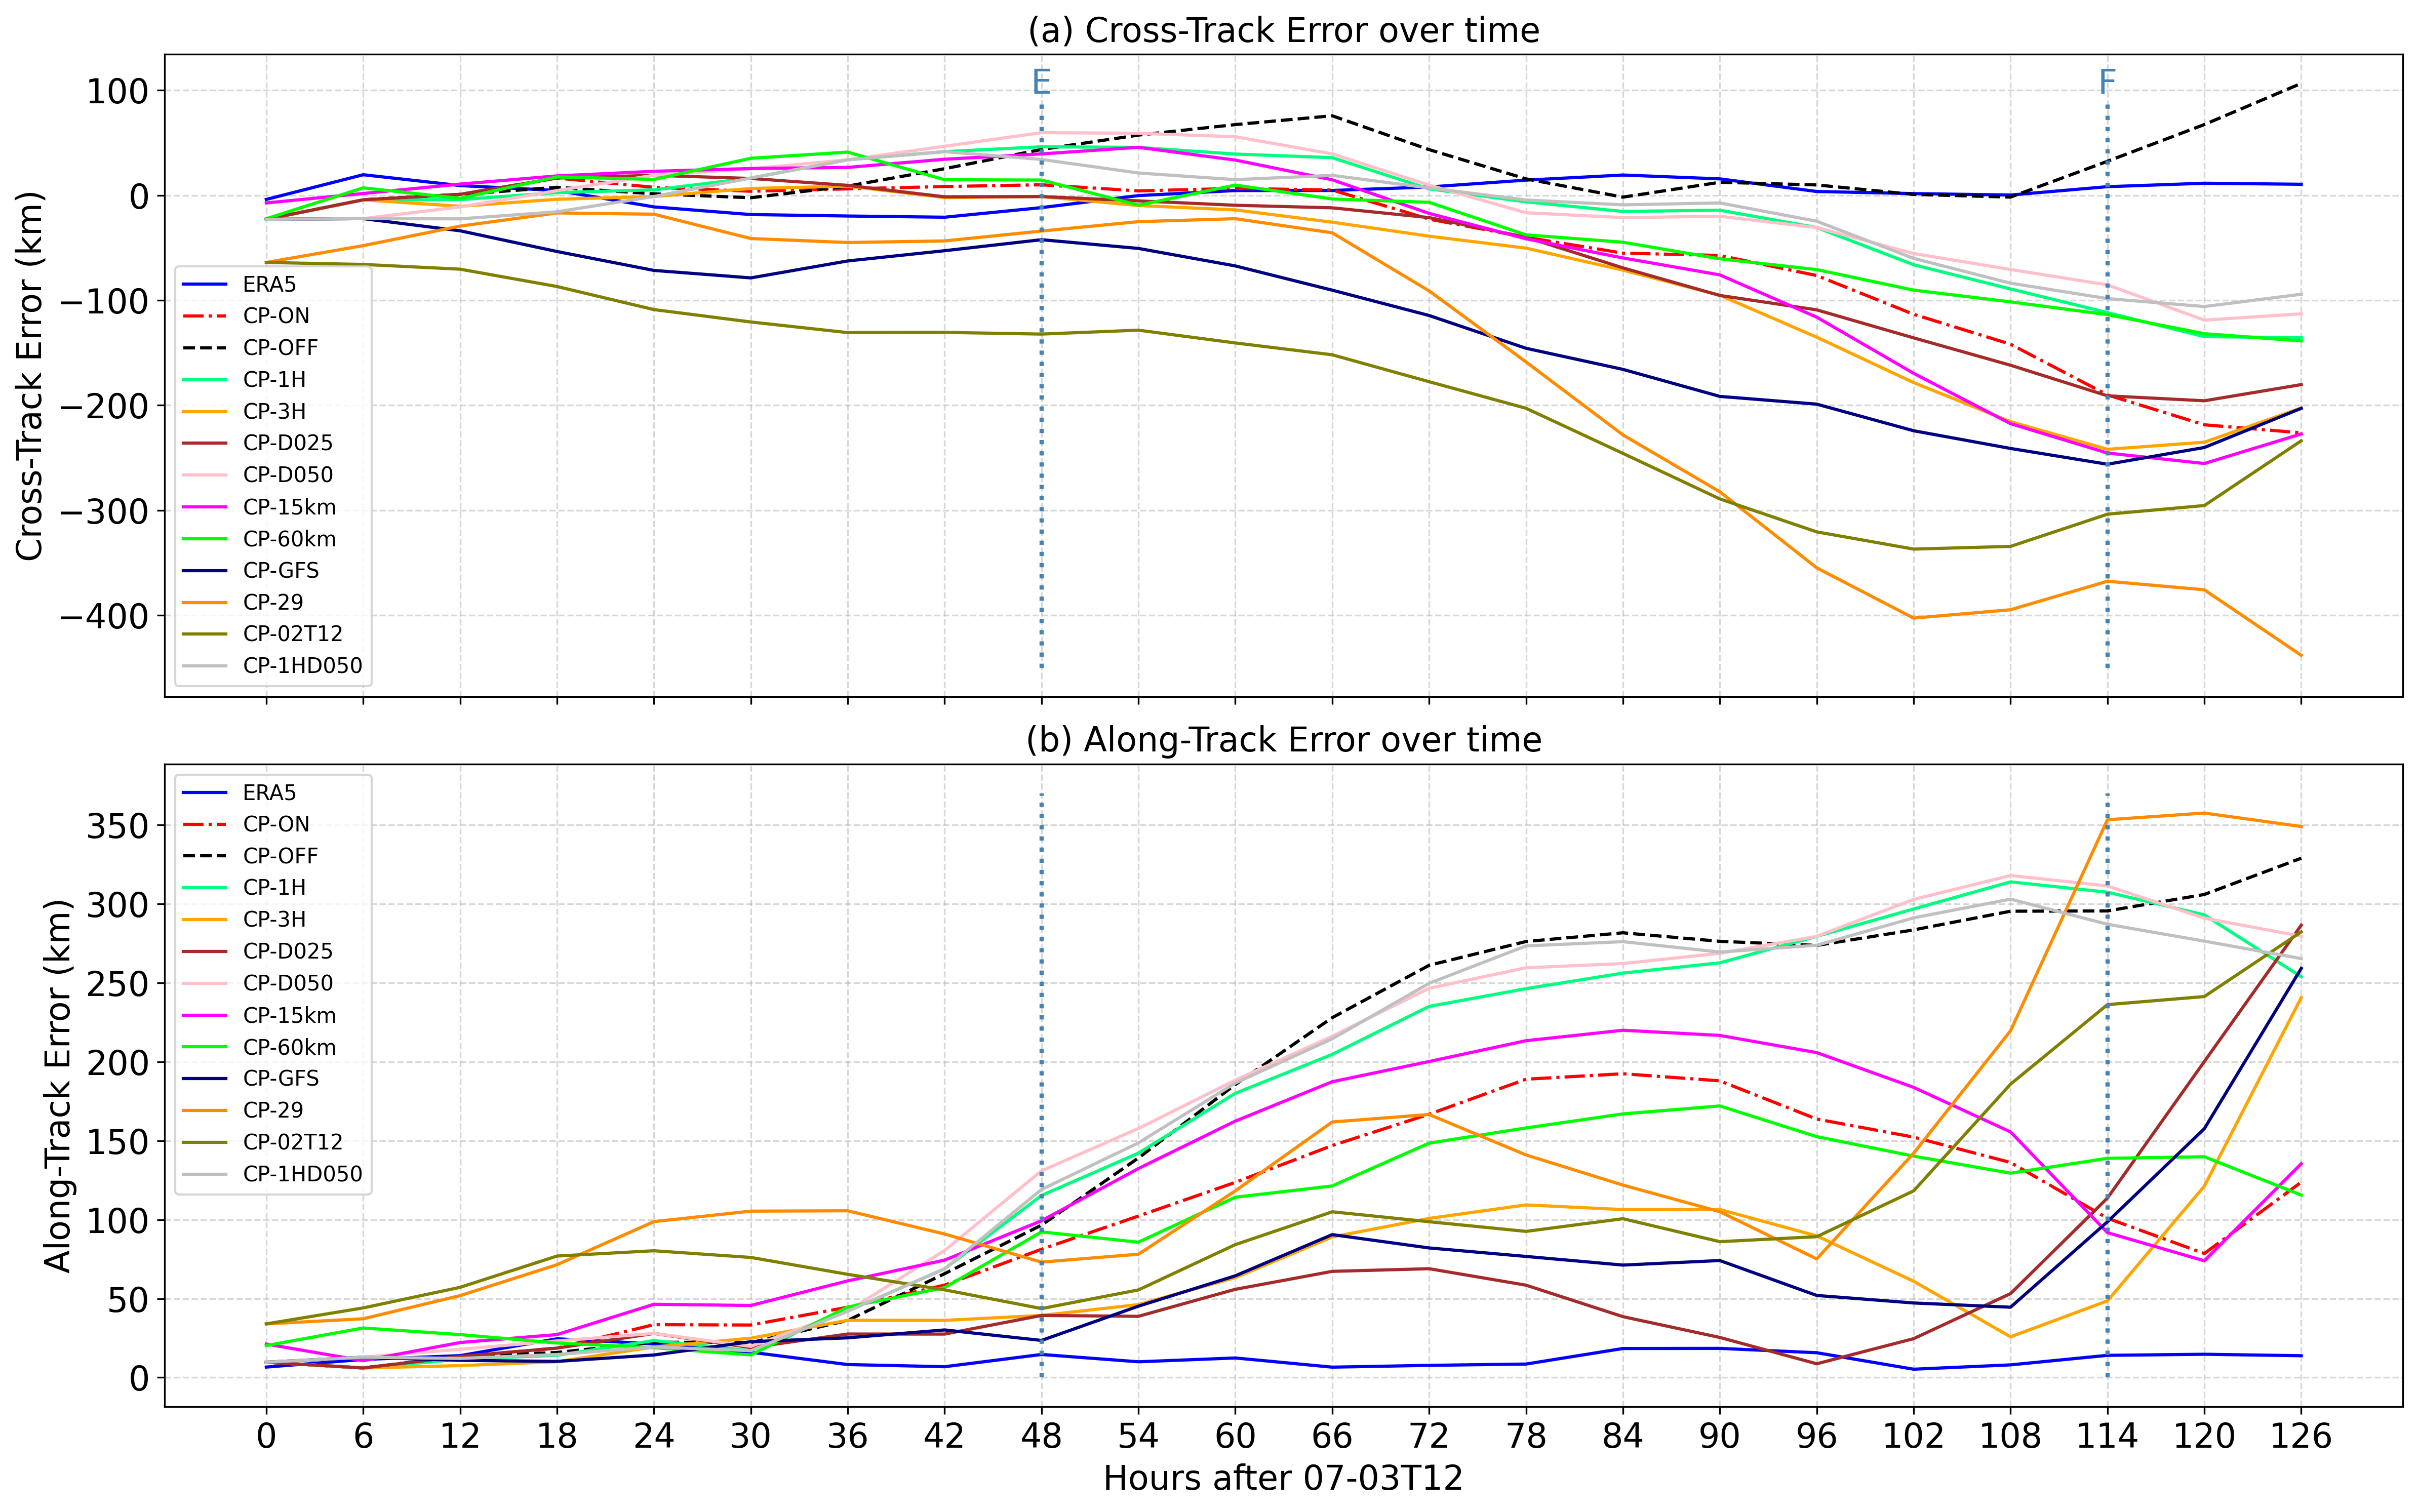
\includegraphics[width=\textwidth]{docs/figuras/chapter5/Cross_Track_Along_Track_Errors_FINAL.png} 
	\vspace{0.5em}
	Source: Made by the author, (2025).  % Fonte abaixo da imagem
	\label{fig:cte} % Label para referenciar no texto
\end{figure}

Overall, most of the forecasts show a negative CTE, meaning there is a leftward (westward) deviation from the observed trajectory, confirming Figure \ref{fig:all_tracks_selected}, which displays all the tracks, and Figure \ref{fig:berryl3rd}. This trend is particularly clear in the CP-02T12 experiment. Since the first hour of the forecast, the CTE is negative, which aligns with the fact that the predicted trajectory is consistently to the left of the observed one.

It is interesting to note that the CTE behavior differs significantly between the CP-ON and CP-OFF experiments. While CP-OFF maintains a positive CTE, CP-ON gradually shifts to a negative CTE as the integration period progresses. Notably, CP-ON begins to deviate leftward after around 72 hours of integration, after passing through the Yucatan Peninsula, whereas in other experiments, such as CP-OFF and CP-D025, this deviation occurs earlier.

Interestingly, despite exhibiting large overall errors (Figure \ref{fig:trackerrors}), the CP-D050 experiment performs better than CP-ON in this metric, as it does not deviate as strongly. This highlights the importance of evaluating forecast performance from multiple perspectives and understanding the sources of these differences, which we will further investigate using meteorological fields.

This westward bias was also noted in the forecasts from both the HAFS (Figure \ref{fig:berryl3rd}) and the UK Met Office  (Figure \ref{fig:metoff}) for Hurricane Beryl.

\begin{figure}[!ht]
	\centering
	\caption{Tracking available by the UK Met Office.} % Título acima da figura
	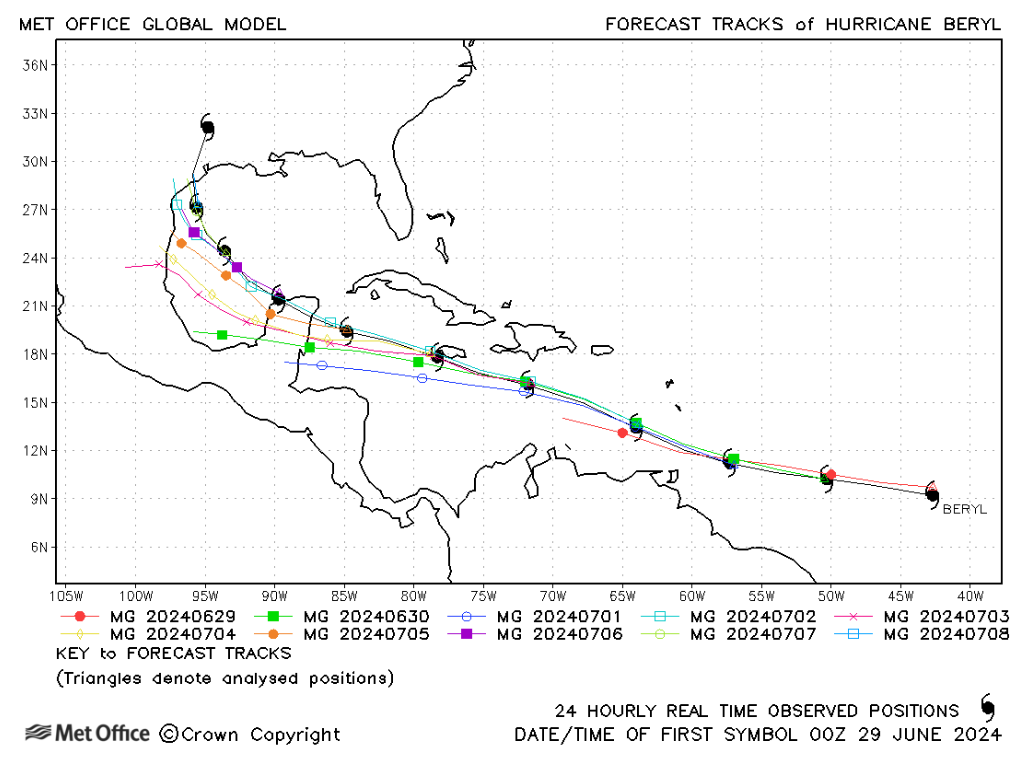
\includegraphics[width=\textwidth]{docs/figuras/chapter5/MetOffice.png} 
	\vspace{0.5em}
	Source: \url{https://www.metoffice.gov.uk/research/weather/tropical-cyclones/verification/seasons/nhem2024.}  % Fonte abaixo da imagem
	\label{fig:metoff} % Label para referenciar no texto
\end{figure}

The report \cite{metoffice2024} indicates that the track was forecasted with a notable degree of accuracy throughout the Caribbean region, furthermore, it was observed that there was a left-of-track bias in the forecasts as Beryl progressed into the Gulf of Mexico.

In general, the ATE is positive across all experiments, indicating a consistent tendency for the MONAN model to move faster than observed. Note that ERA5 also displays this trend, though it is not as pronounced as in MONAN.

When comparing CP-ON and CP-OFF, a growing ATE trend is evident in CP-OFF. As the integration period increases, CP-OFF moves increasingly ahead of the observed track, reaching 225 km ahead at 66 hours, whereas CP-ON is only about 150 km ahead at the same time.

The CP-D025 experiment appears to be more in phase with the observations in this metric than CP-ON during most of the forecast period, despite having a greater leftward deviation compared to CP-ON. Despite larger errors in track positioning, the early-initialized forecasts manage to better match the best track in terms of propagation speed. In this case, the forecast initialized with GFS outperformed the forecast initialized with ERA5 during most of the integration period.

A mean error performance of all MONAN forecasts were computed and shown at Figure \ref{fig:monera5}.

\begin{figure}[!ht]
	\centering
	\caption{Overall performance of MONAN trajectory forecasts compared with ERA5 reanalysis.} % Título acima da figura
	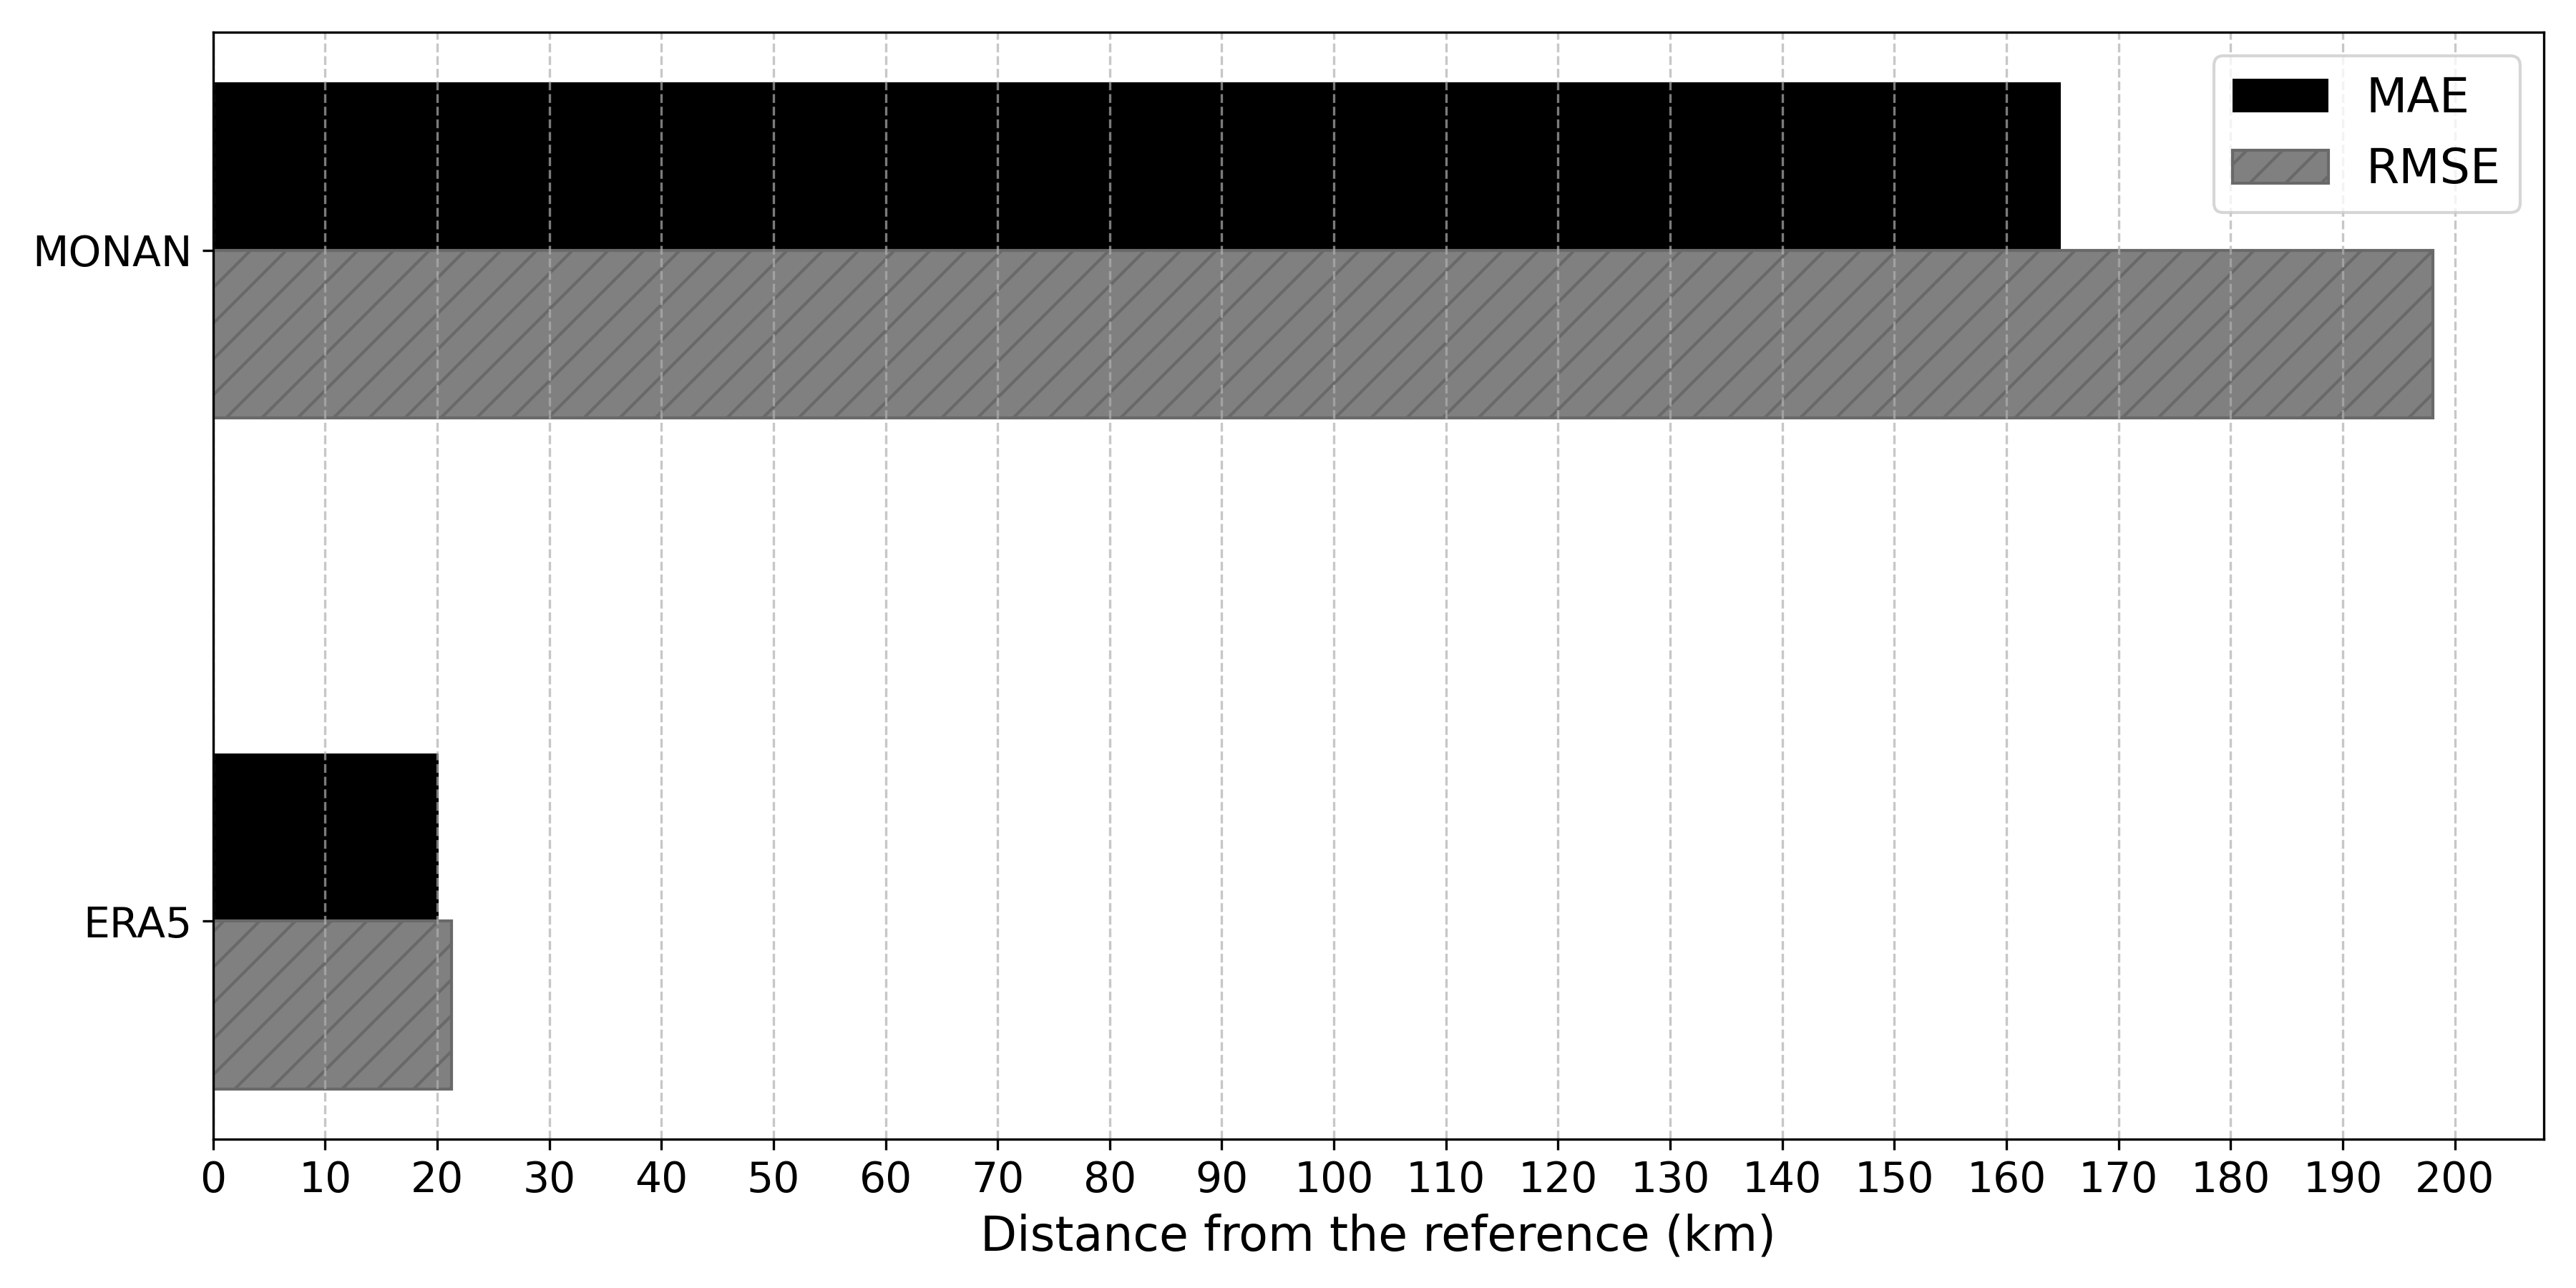
\includegraphics[width=\textwidth]{docs/figuras/chapter5/barplot_monan_vs_era5_mae_rmse_FINAL.png} 
	\vspace{0.5em}
	Source: Made by the author (2025).  % Fonte abaixo da imagem
	\label{fig:monera5} % Label para referenciar no texto
\end{figure}

In general, the MONAN forecast is approximately 8 times greater than the ERA5 reanalysis. Again, we can infer that it is not a fair comparison between the MONAN forecast and the ERA5 reanalysis, but it is important to notice the error scale to give us insights about improving the MONAN forecast.




\subsection{Intensity}




\subsection{Rainfall}

\subsubsection{Pattern and spatial rainfall distribution}

\subsubsection{Rainfall mean and overall distribution}

\subsubsection{MONAN performance at forecasting rainfall}

\subsection{Discussion of key outcomes}

 %% DATA
\chapter{CONCLUSIONS AND FUTURE WORK}
\label{ch:conclusion}

\section{Future Work}

\chapter{CONCLUSIONS AND FUTURE WORK}
\label{ch:conclusion}

\section{Future Work}
  

%%%%%%%%%%%%%%%%%%%%%%%%%%%%%%%%%%%%%%%%%%%%%%%%%%%%%%
% %Apêndice A
\hypertarget{estilo:apendice}{} %% uso para este Guia
%Este apêndice foi criado apenas para indicar como construir um apêndice no estilo, não existia no original da tese.
%%%%%%%%%%%%%%%%%%%%%%%%%%%%%%%%%%%%%%%%%%%%%%%%%%%%%%
\renewcommand{\thechapter}{A} % Define a letra A como identificador do capítulo
\chapter{APPENDIX - THE MASS FLUX DEDUCTION}
\label{appendixA}


Here is briefly described the mass flux approach in the cold pool parameterization context.


\chapter{APPENDIX B - THE TRACKING ALGORITHM}
\label{appendixB}
Descrever o algoritmo assim como referencias.

%% insira quantos capítulos desejar com o seguinte comando:
%\include{_pasta_do_arquivo_/_meu_arquivo_} %%sem a extensão
%% note que deverá haver um arquivo _meu_arquivo_.tex (com extensão) no diretório _pasta_do_arquivo_

% PARA PUBLICAÇÕES EM INGLÊS:
%% Descomentar essa linha para publicações em inglês
%\bibliographystyle{./template/abnt-alfenglish}

% PARA PUBLICAÇÕES EM PORTUGUÊS:
%% comentar essa linha para publicações em inglês
\bibliographystyle{./template/abnt-alfportuguese}

%% Bibliografia %% não alterar %% obrigatório %testebib
\bibliography{./bib/referencia} %% aponte para seu arquivo de bibliografia no formato bibtex (p.ex: referencia.bib)

%\include{./docs/09_glossario} %% insira os termos do glossário no arquivo glossario.tex %% opcional

%\inicioApendice %% opcional, comente esta linha e a seguintes se não houver apendice(s)
%\include{./docs/10_01_apendice1} %% insira apendices tal qual capítulos acima

%\inicioAnexo
%%%%%%%%%%%%%%%%%%%%%%%%%%%%%%%%%%%%%%%%%%%%%%%%%%%%%%%
%Anexo
%Este anexo foi incluido para explicar como incluir um anexo no estilo, não existia no original desta tese.
%%%%%%%%%%%%%%%%%%%%%%%%%%%%%%%%%%%%%%%%%%%%%%%%%%%%%%%%%%%%%%%%%%%%%%%%%%%%%%%%%
\renewcommand{\thechapter}{}%
\chapter{ANEXO A - ABREVIATURA DOS MESES} %% Título do anexo sempre em maiúsculas. Trocar A por B no próximo anexo e etc
\label{anexoA} %% Rótulo aplicado caso queira referir-se a este tópico em qualquer lugar do texto. Trocar A por B no próximo anexo e etc
\renewcommand{\thechapter}{A}%		% trocar A por B no próximo anexo e etc

\begin{table}[!ht]
 \label{tab:abreviaturas}
  \begin{center}
 	\begin{tabular}{lll}
	 \hline
	  \textbf{Português}    & \textbf{Espanhol}  & \textbf{Italiano}\\ 
   \hline
       janeiro   = jan.   & enero = ene.       & gennaio = gen.\\
       fevereiro = fev.   & febrero = feb.     & febbraio = feb.\\
       março     = mar.   & marzo = mar.       & marzo = mar.\\
       abril     = abr.   & abril = abr.       & aprile = apr.\\
       maio      = maio   & mayo = mayo        & maggio = mag.\\ 
       junho     = jun.   & junio = jun.       & giugno = giu.\\ 
       julho     = jul.   & julio = jul.       & luglio = lug.\\
       agosto    = ago.   & agosto = ago.      & agosto = ago.\\
       setembro  = set.   & septiembre = sep.  & settembre = set.\\
       outubro   = out.   & octubre = oct.     & ottobre = ott.\\
       novembro  = nov.   & noviembre =nov.    & novembre = nov.\\
       dezembro  = dez.   & diciembre = dic.   & dicembre = dic.\\ 
     \hline
   \textbf{Francês}       & \textbf{Inglês}    & \textbf{Alemão}\\
     \hline
       janvier = jan.     & January = Jan.     & Januar = Jan.\\
       février = fév.     & February = Feb.    & Februar = Feb.\\
       mars = mars        & March = Mar.       & März = März\\
       avril = avr.       & April = Apr.       & April = Apr.\\
       mai = mai          & May = May          & Mai = Mai.\\
       juin = juin        & June = June        & Juni = Juni\\
       juillet = juil.    & July = July        & Juli = Juli\\
       août = août        & August = Aug.      & August = Aug.\\
       septembre = sept.  & September = Sept.  & September = Sept.\\
       octobre = oct.     & October = Oct.     & Oktober = Okt.\\
       novembre = nov.    & November = Nov.    & November = Nov.\\
       décembre = déc.    & December = Dec.    & Dezember = Dez. \\ 
    \hline
   \end{tabular}
   \end{center}
	 \FONTE{Adaptada de \citeonline[p.~22]{NBR6023:2002b}.}
\end{table}
%%%%%%%%%%%%%%%%%%%%%%%%%%%%%%%%%%%%%%%%%%%%%%%%%%%%%%%%
%Anexo
%Este anexo foi incluido para explicar como incluir um anexo no estilo, não existia no original desta tese
%exceto algumas tabelas que foram modificadas
%%%%%%%%%%%%%%%%%%%%%%%%%%%%%%%%%%%%%%%%%%%%%%%%%%%%%%%%%%%%%%%%%%%%%%%%%%%%%%%%%
\renewcommand{\thechapter}{}%
\chapter{ANEXO B - EXEMPLOS DE FIGURAS E TABELAS NO \LaTeX} %% Título do anexo sempre em maiúsculas.
\label{anexoB} %% Rótulo aplicado caso queira referir-se a este tópico em qualquer lugar do texto.
\renewcommand{\thechapter}{B}%

\section{Figuras} %% Título de secção sempre com as primeiras letras em maiúsculas.
\label{anexo2}

\begin{figure}[ht]
	\caption{Exemplo de figura com título curto.}
	\vspace{6mm}	% acrescentar o espaçamento vertical apropriado entre o título e a borda superior da figura
	\begin{center}
    	\includegraphics[width=\mylenfig]{docs/figuras/gpa.pdf}  
	\end{center}
	\vspace{4mm}	% acrescentar o espaçamento vertical apropriado entre a borda inferior da figura e a legenda ou a fonte quando não há legenda (o valor pode ser negativo para subir)
	\legenda{Exemplo de legenda curta.}	% legenda - opcional
	\label{figgpa1}
	\FONTE{\citeonline{lba/06}.}	% fonte consultada (elemento obrigatório, mesmo que seja produção do próprio autor)
\end{figure}

\begin{figure}[!h]
	\caption{Figura com título que ocupa mais de uma linha, alinhar as demais com a primeira
letra depois do hífen.}
%o ajuste do título é feito automaticamente pelo \LaTeX\ caso este ocupe mais de uma linha.}
	\vspace{6mm}	% acrescentar o espaçamento vertical apropriado entre o título e a borda superior da figura
	\begin{center}
    	\includegraphics[width=\mylenfig]{docs/figuras/gpa.pdf}  
	\end{center}
	\vspace{4mm}	% acrescentar o espaçamento vertical apropriado entre a borda inferior da figura e a legenda ou a fonte quando não há legenda (o valor pode ser negativo para subir)
	\legenda{Exemplo de legenda que ocupa mais de uma linha, alinhar as demais com a primeira
letra da primeira linha.}	% legenda - opcional
%o \LaTeX\ alinha o texto automaticamente.
	\label{figgpa2}
	\FONTE{Se o texto da fonte for longo e ocupar mais de uma linha as demais ficam alinhadas
	com a palavra fonte. Adaptada de \citeonline{mauri:2003}.}	% fonte consultada (elemento obrigatório, mesmo que seja produção do próprio autor)
%o \LaTeX\ alinha o texto automaticamente.
\end{figure}

\clearpage
\section{Tabelas} 

\begin{table}[!ht]%[htbp] %opções de colocação da tabela no texto
  \begin{center}	% use sempre um ambiente para as tabelas
									% (opções: center (recomendado), flushright, flushleft)
									% NÃO USE \centering com TABELAS se houver \FONTE!	
  \caption{Exemplo de tabela, com fonte.}
    \begin{tabular}{l|l|c|c|r|r}
			\hline % desenha uma linha horizontal
				Campo 1 & Campo2 & Campo3 & Campo 4 & Campo5 & Campo6 \\
				Campo 1 & Campo2 & Campo3 & Campo 4 & Campo5 & Campo6 \\
				Campo 1 & Campo2 & Campo3 & Campo 4 & Campo5 & Campo6 \\				
			\hline % desenha uma linha horizontal
    \end{tabular}
    \end{center}
 \FONTE{Coloque a fonte de referência aqui, se houver.}
\end{table}

% \hhline{|--|} \multicolumn{2}{|c|}{continuação da página anterior} \\
% \hhline{|--|} \endhead % ate aqui eh definicao do "head" da pagina 
%   % dois em diante
% \hhline{|--|} \multicolumn{2}{|c|}{continua para próxima página} \\
% \hhline{|--|} \endfoot % ate aqui eh definicao do "foot" exceto ultima página
% \hhline{|b:=:=:b|} \endlastfoot % ate aqui eh definicao do "foot" 
%   % da ultima pagina

\begin{table}[hb]
\renewcommand{\baselinestretch}{1.4}% for tabular environment
\small
   \centering
   \caption{Exemplo de tabela, com fonte longa}
%   \label{\fullpaperid:table:1}% you must prefix your labels (here table:1) with the string \fullpaperid: (this will be important when combining all the full papers for the final book)
	\begin{center}
	   \begin{tabular}{lcc}
	       \hline% horizontal line
	       \itshape Parameter&
	           \itshape $\kappa$ Scaling&
	           \itshape $\kappa$, $\lambda$ Scaling\\*
	       \hline
	       Dimension&
	           $\kappa^{-1}$&
	           $\lambda^{-1}$\\*
	       Currant&
	           $\kappa^{-1}$&
	               $\lambda/\kappa^{2}$\\*
	       Dopant Concentration&
	           $\kappa$&
	           $\lambda2/\kappa$\\*
	       \hline
	   \end{tabular}
	\end{center}
    \renewcommand{\baselinestretch}{1.0}
    \FONTE{Coloque a fonte longa longa longa longa longa longa longa longa longa longa aqui, se houver.}
\end{table}

% Exemplos de 2 tabelas avançadas 

\begin{table}[ht!]
\caption{Outro exemplo de tabela}
%\label{\fullpaperid:table:2}
\begin{center}
\renewcommand{\baselinestretch}{1.2}% for tabular environment
\small
\begin{tabular}{cccccc}
\hline
   & \multirow{2}{22mm}{\renewcommand{\baselinestretch}{0.7}\small\centering Quantitative measures} & \multicolumn{4}{c}{Markers} \\ \cline{3-6}
   & & \multicolumn{1}{c}{RO} & \multicolumn{1}{c}{ASF} & \multicolumn{1}{c}{ISO} & \multicolumn{1}{c}{ADF} \\ \hline
   \multirow{3}{20mm}{\renewcommand{\baselinestretch}{0.7}\small\centering Test image scale 2}
& RMSE & 0.126 & 0.187 & 0.118 & 0.103 \\
& NMSE & 0.046 & 0.101 & 0.040 & 0.031 \\
& SSIM & 0.9981 & 0.9956 & 0.9984 & 0.9989 \\ \hline
   \multirow{3}{18mm}{\renewcommand{\baselinestretch}{0.7}\small\centering Cameraman scale 4}
& RMSE & 13.748 & 15.649 & 10.132 & 4.325 \\
& NMSE & 0.011 & 0.014 & 0.006 & 0.001 \\
& SSIM & 0.923 & 0.847 & 0.904 & 0.933 \\ \hline
   \multirow{3}{18mm}{\renewcommand{\baselinestretch}{0.7}\small\centering Cameraman scale 7}
& RMSE & 20.963 & 22.652 & 13.108 & 4.650 \\
& NMSE & 0.024 & 0.029 & 0.010 & 0.001 \\
& SSIM & 0.851 & 0.757 & 0.866 & 0.925 \\ \hline
   \multirow{3}{23mm}{\renewcommand{\baselinestretch}{1.2}\small\centering Crop of cameraman scale 7}
& RMSE & 30.914 & 31.943 & 17.831 & 2.870 \\
& NMSE & 0.053 & 0.057 & 0.018 & 0.001 \\
& SSIM & 0.831 & 0.772 & 0.891 & 0.983 \\ \hline
\end{tabular}
\end{center}
\end{table}

\begin{table}[ht!]
\caption{Mais um exemplo de tabela}
%\label{\fullpaperid:table:1}
\begin{center}
\renewcommand{\baselinestretch}{1.2}% for tabular environment
\small
\begin{tabular}{ccccc}
\hline
\multirow{4}{16mm}{\renewcommand{\baselinestretch}{0.7}\small\centering Leveling's Scale} & \multicolumn{4}{c}{Values for the scale relation of the four different type of markers} \\ \cline{2-5}
& \multirow{3}{29mm}{\renewcommand{\baselinestretch}{1}\small\centering Structure element's size $r$ for RO and ASF} & \multicolumn{2}{c}{Isotropic diffusion} & \multirow{3}{20mm}{\renewcommand{\baselinestretch}{1}\small\centering Anisotropic diffusion iterations $t$} \\ \cline{3-4}
& & \multirow{2}{23mm}{\renewcommand{\baselinestretch}{0.7}\small\centering Standard deviation $\sigma$} & \multirow{2}{12mm}{\renewcommand{\baselinestretch}{0.7}\small\centering Kernel size} & \\
& & & & \\ \hline
1 & 1 & 0.5 & $5 \times 5$ & 100 \\
2 & 2 & 1.0 & $7 \times 7$ & 200 \\
3 & 3 & 1.5 & $11 \times 11$ & 300 \\
4 & 4 & 2.0 & $13 \times 13$ & 400 \\
5 & 5 & 2.5 & $17 \times 17$ & 500 \\
6 & 6 & 3.0 & $19 \times 19$ & 600 \\
7 & 7 & 3.5 & $23 \times 23$ & 700 \\ \hline
\end{tabular}
\end{center}
\end{table} 

\setlongtables

\begin{longtable}[c]{c|c|c|c|c|c}
\caption{Exemplo de tabela longa que atravessa várias páginas.}\label{tab:longas}\\
\hline
\textbf{Campo1} & \textbf{Campo2} & \textbf{Campo3} & \textbf{Campo4} & \textbf{Campo5} & \textbf{Campo6} \\
\hline\hline
\endfirsthead

\endlastfoot
\hline
\multicolumn{6}{r}{\captionlabelfont\captionsize(Continua)}\\
\endfoot

	campo1 & campo2 & campo3 & campo4 & campo5 & campo6 \\
	campo1 & campo2 & campo3 & campo4 & campo5 & campo6 \\
	campo1 & campo2 & campo3 & campo4 & campo5 & campo6 \\
	campo1 & campo2 & campo3 & campo4 & campo5 & campo6 \\
	campo1 & campo2 & campo3 & campo4 & campo5 & campo6 \\
	campo1 & campo2 & campo3 & campo4 & campo5 & campo6 \\
	campo1 & campo2 & campo3 & campo4 & campo5 & campo6 \\
	campo1 & campo2 & campo3 & campo4 & campo5 & campo6 \\
	campo1 & campo2 & campo3 & campo4 & campo5 & campo6 \\
	campo1 & campo2 & campo3 & campo4 & campo5 & campo6 \\
	campo1 & campo2 & campo3 & campo4 & campo5 & campo6 \\
	campo1 & campo2 & campo3 & campo4 & campo5 & campo6 \\
	campo1 & campo2 & campo3 & campo4 & campo5 & campo6 \\
	campo1 & campo2 & campo3 & campo4 & campo5 & campo6 \\
	campo1 & campo2 & campo3 & campo4 & campo5 & campo6 \\
	campo1 & campo2 & campo3 & campo4 & campo5 & campo6 \\
	campo1 & campo2 & campo3 & campo4 & campo5 & campo6 \\
	campo1 & campo2 & campo3 & campo4 & campo5 & campo6 \\
	campo1 & campo2 & campo3 & campo4 & campo5 & campo6 \\
	campo1 & campo2 & campo3 & campo4 & campo5 & campo6 \\

\noalign{\makeatletter\global\setbox9\box\LT@head}
\pagebreak
\multicolumn{6}{c}{Tabela \ref{tab:longas} - Continuação} \\*
\hline
\textbf{Campo1} & \textbf{Campo2} & \textbf{Campo3} & \textbf{Campo4} & \textbf{Campo5} & \textbf{Campo6} \\
\hline\hline

	campo1 & campo2 & campo3 & campo4 & campo5 & campo6 \\
	campo1 & campo2 & campo3 & campo4 & campo5 & campo6 \\
	campo1 & campo2 & campo3 & campo4 & campo5 & campo6 \\
	campo1 & campo2 & campo3 & campo4 & campo5 & campo6 \\
	campo1 & campo2 & campo3 & campo4 & campo5 & campo6 \\
	campo1 & campo2 & campo3 & campo4 & campo5 & campo6 \\
	campo1 & campo2 & campo3 & campo4 & campo5 & campo6 \\
	campo1 & campo2 & campo3 & campo4 & campo5 & campo6 \\
	campo1 & campo2 & campo3 & campo4 & campo5 & campo6 \\
	campo1 & campo2 & campo3 & campo4 & campo5 & campo6 \\
	campo1 & campo2 & campo3 & campo4 & campo5 & campo6 \\
	campo1 & campo2 & campo3 & campo4 & campo5 & campo6 \\
	campo1 & campo2 & campo3 & campo4 & campo5 & campo6 \\
	campo1 & campo2 & campo3 & campo4 & campo5 & campo6 \\
	campo1 & campo2 & campo3 & campo4 & campo5 & campo6 \\
	campo1 & campo2 & campo3 & campo4 & campo5 & campo6 \\
	campo1 & campo2 & campo3 & campo4 & campo5 & campo6 \\
	campo1 & campo2 & campo3 & campo4 & campo5 & campo6 \\
	campo1 & campo2 & campo3 & campo4 & campo5 & campo6 \\
	campo1 & campo2 & campo3 & campo4 & campo5 & campo6 \\
	campo1 & campo2 & campo3 & campo4 & campo5 & campo6 \\
	campo1 & campo2 & campo3 & campo4 & campo5 & campo6 \\
	campo1 & campo2 & campo3 & campo4 & campo5 & campo6 \\
	campo1 & campo2 & campo3 & campo4 & campo5 & campo6 \\
	campo1 & campo2 & campo3 & campo4 & campo5 & campo6 \\
	campo1 & campo2 & campo3 & campo4 & campo5 & campo6 \\
	campo1 & campo2 & campo3 & campo4 & campo5 & campo6 \\
	campo1 & campo2 & campo3 & campo4 & campo5 & campo6 \\
	campo1 & campo2 & campo3 & campo4 & campo5 & campo6 \\
	campo1 & campo2 & campo3 & campo4 & campo5 & campo6 \\
	campo1 & campo2 & campo3 & campo4 & campo5 & campo6 \\
	campo1 & campo2 & campo3 & campo4 & campo5 & campo6 \\
	campo1 & campo2 & campo3 & campo4 & campo5 & campo6 \\
	campo1 & campo2 & campo3 & campo4 & campo5 & campo6 \\
	
\noalign{\makeatletter\global\setbox9\box\LT@head}
\pagebreak
\multicolumn{6}{c}{Tabela \ref{tab:longas} - Conclusão} \\*
\hline
\textbf{Campo1} & \textbf{Campo2} & \textbf{Campo3} & \textbf{Campo4} & \textbf{Campo5} & \textbf{Campo6} \\
\hline\hline

	campo1 & campo2 & campo3 & campo4 & campo5 & campo6 \\
	campo1 & campo2 & campo3 & campo4 & campo5 & campo6 \\
	campo1 & campo2 & campo3 & campo4 & campo5 & campo6 \\
	campo1 & campo2 & campo3 & campo4 & campo5 & campo6 \\
	campo1 & campo2 & campo3 & campo4 & campo5 & campo6 \\
	campo1 & campo2 & campo3 & campo4 & campo5 & campo6 \\
	campo1 & campo2 & campo3 & campo4 & campo5 & campo6 \\
	campo1 & campo2 & campo3 & campo4 & campo5 & campo6 \\
	campo1 & campo2 & campo3 & campo4 & campo5 & campo6 \\
	campo1 & campo2 & campo3 & campo4 & campo5 & campo6 \\
	campo1 & campo2 & campo3 & campo4 & campo5 & campo6 \\
	campo1 & campo2 & campo3 & campo4 & campo5 & campo6 \\
	campo1 & campo2 & campo3 & campo4 & campo5 & campo6 \\
	campo1 & campo2 & campo3 & campo4 & campo5 & campo6 \\
	campo1 & campo2 & campo3 & campo4 & campo5 & campo6 \\
	campo1 & campo2 & campo3 & campo4 & campo5 & campo6 \\
	campo1 & campo2 & campo3 & campo4 & campo5 & campo6 \\
	campo1 & campo2 & campo3 & campo4 & campo5 & campo6 \\
	campo1 & campo2 & campo3 & campo4 & campo5 & campo6 \\
\hline
\end{longtable}
% o comando \FONTE{} não pode ser usado neste caso
\vspace{-8mm}
\begin{center}
	Fonte: Referência a fonte da tabela.
\end{center}


A \autoref{tab:longa} é um exemplo de tabela no modo paisagem e que ocupa também várias páginas.

\setlongtables
\begin{landscape}
\begin{longtable}[c]{c|c|c|c|c|c|c|c|c|c}
\caption{Exemplo de tabela longa, em paisagem, que atravessa várias páginas.}\label{tab:longa}\\
\hline
\textbf{BOX1} & \textbf{BOX2} & \textbf{BOX3} & \textbf{BOX4} & \textbf{BOX5} & \textbf{BOX6} & \textbf{BOX7} & \textbf{BOX8} & \textbf{BOX9} & \textbf{BOX10} \\
\hline\hline
\endfirsthead
\caption[]{Conclusão}\\
\hline
\textbf{BOX1} & \textbf{BOX2} & \textbf{BOX3} & \textbf{BOX4} & \textbf{BOX5} & \textbf{BOX6} & \textbf{BOX7} & \textbf{BOX8} & \textbf{BOX9} & \textbf{BOX10} \\
\hline\hline
\endhead
\endlastfoot
\hline
\multicolumn{10}{r}{\captionlabelfont\captionsize(Continua)}\\
\endfoot
	
	BOX1 & BOX2 & BOX3 & BOX4 & BOX5 & BOX6 & BOX7 & BOX8 & BOX9 & BOX10 \\
	BOX1 & BOX2 & BOX3 & BOX4 & BOX5 & BOX6 & BOX7 & BOX8 & BOX9 & BOX10 \\
	BOX1 & BOX2 & BOX3 & BOX4 & BOX5 & BOX6 & BOX7 & BOX8 & BOX9 & BOX10 \\
	BOX1 & BOX2 & BOX3 & BOX4 & BOX5 & BOX6 &	BOX7 & BOX8 & BOX9 & BOX10 \\
	BOX1 & BOX2 & BOX3 & BOX4 & BOX5 & BOX6 &	BOX7 & BOX8 & BOX9 & BOX10 \\
	BOX1 & BOX2 & BOX3 & BOX4 & BOX5 & BOX6 &	BOX7 & BOX8 & BOX9 & BOX10 \\
	BOX1 & BOX2 & BOX3 & BOX4 & BOX5 & BOX6 &	BOX7 & BOX8 & BOX9 & BOX10 \\
	BOX1 & BOX2 & BOX3 & BOX4 & BOX5 & BOX6 &	BOX7 & BOX8 & BOX9 & BOX10 \\
	BOX1 & BOX2 & BOX3 & BOX4 & BOX5 & BOX6 &	BOX7 & BOX8 & BOX9 & BOX10 \\
	BOX1 & BOX2 & BOX3 & BOX4 & BOX5 & BOX6 &	BOX7 & BOX8 & BOX9 & BOX10 \\
	BOX1 & BOX2 & BOX3 & BOX4 & BOX5 & BOX6 & BOX7 & BOX8 & BOX9 & BOX10 \\
	BOX1 & BOX2 & BOX3 & BOX4 & BOX5 & BOX6 &	BOX7 & BOX8 & BOX9 & BOX10 \\
	BOX1 & BOX2 & BOX3 & BOX4 & BOX5 & BOX6 &	BOX7 & BOX8 & BOX9 & BOX10 \\
	BOX1 & BOX2 & BOX3 & BOX4 & BOX5 & BOX6 &	BOX7 & BOX8 & BOX9 & BOX10 \\
	BOX1 & BOX2 & BOX3 & BOX4 & BOX5 & BOX6 &	BOX7 & BOX8 & BOX9 & BOX10 \\
	BOX1 & BOX2 & BOX3 & BOX4 & BOX5 & BOX6 &	BOX7 & BOX8 & BOX9 & BOX10 \\
	BOX1 & BOX2 & BOX3 & BOX4 & BOX5 & BOX6 &	BOX7 & BOX8 & BOX9 & BOX10 \\
	BOX1 & BOX2 & BOX3 & BOX4 & BOX5 & BOX6 &	BOX7 & BOX8 & BOX9 & BOX10 \\
	BOX1 & BOX2 & BOX3 & BOX4 & BOX5 & BOX6 &	BOX7 & BOX8 & BOX9 & BOX10 \\                                 
	BOX1 & BOX2 & BOX3 & BOX4 & BOX5 & BOX6 &	BOX7 & BOX8 & BOX9 & BOX10 \\
	BOX1 & BOX2 & BOX3 & BOX4 & BOX5 & BOX6 &	BOX7 & BOX8 & BOX9 & BOX10 \\
	BOX1 & BOX2 & BOX3 & BOX4 & BOX5 & BOX6 &	BOX7 & BOX8 & BOX9 & BOX10 \\
	BOX1 & BOX2 & BOX3 & BOX4 & BOX5 & BOX6 &	BOX7 & BOX8 & BOX9 & BOX10 \\
	BOX1 & BOX2 & BOX3 & BOX4 & BOX5 & BOX6 &	BOX7 & BOX8 & BOX9 & BOX10 \\
	BOX1 & BOX2 & BOX3 & BOX4 & BOX5 & BOX6 &	BOX7 & BOX8 & BOX9 & BOX10 \\
	BOX1 & BOX2 & BOX3 & BOX4 & BOX5 & BOX6 &	BOX7 & BOX8 & BOX9 & BOX10 \\
	BOX1 & BOX2 & BOX3 & BOX4 & BOX5 & BOX6 &	BOX7 & BOX8 & BOX9 & BOX10 \\
	BOX1 & BOX2 & BOX3 & BOX4 & BOX5 & BOX6 &	BOX7 & BOX8 & BOX9 & BOX10 \\
\hline
\end{longtable}
\vspace{-8mm}
% o comando \FONTE{} não pode ser usado neste caso
\begin{center}
	Fonte: Referência a fonte da tabela.
\end{center}
\end{landscape}
%%%%%%%%%%%%%%%%%%%%%%%%%%%%%%%%%%%%%%%%%%%%%%%%%%%%%%%
%Anexo
%Este anexo foi incluido para explicar como incluir um anexo no estilo, não existia no original desta tese.
%%%%%%%%%%%%%%%%%%%%%%%%%%%%%%%%%%%%%%%%%%%%%%%%%%%%%%%%%%%%%%%%%%%%%%%%%%%%%%%%%
\renewcommand{\thechapter}{}%
\chapter{ANEXO C - TIPOS DE REFERÊNCIAS NO \LaTeX} %% Título do anexo sempre em maiúsculas.
\label{anexoC} %% Rótulo aplicado caso queira referir-se a este tópico em qualquer lugar do texto.
\renewcommand{\thechapter}{C}%

\begin{verbatim}

@BOOK{aacr2004, 
  title = {Cataloga{\c{c}}{\~a}o de recursos bibliogr{\'a}ficos 
  pelo {AACR2R} 2002}, 
  edition = {2},
  address = {Bras{\'i}lia},
  publisher = {Editora do Autor},
  author = {Antonia Motta Castro Memória Ribeiro},
  year = {2004}, 
  note = {v{\'a}rias p{\'a}gina{\c{c}}{\~o}es},
 }

@BOOK{rey93,
  title = {Planejar e redigir trabalhos cient\'ificos},
	subtitle = {teste de subtítulo},
  publisher = {Edgard Blücher},
  year = {1993},
  author = {Rey, L.},
  address = {S\~ao Paulo},
  pages = {318},
} 

@MISC{adobe00,
  title = {Adobe Acrobat 5.0.},
  year = {2000},
  note = {1 CD-ROM},
  address = {San Jose, CA},
  publisher = {Adobe Systems},
}


@ARTICLE{amaral98,
  author = {J. R. Amaral},
  title = {{INPE} estuda queda de meteorito na {A}maz{\^o}nia},
  journal = {Jornal Valeparaibano},
  year = {1998},
  month = {22 mar.},
  note = {Caderno 1, p. 12},
  address = {S{\~a}o Jos{\'e} dos Campos},}
}

@BOOK{assireu03,
  title = {Aplica{\c{c}}{\~a}o do operador de fragmenta{\c{c}}{\~a}o  
  assim{\'e}trica {(FA)} na caracteriza{\c{c}}{\~a}o de controles 
  geomorfol{\'o}gicos em reservat{\'o}rios hidrel{\'e}tricos},
  publisher = {INPE},
  year = {2003},
  author = {A. T. Assireu and E. M. L. M. Novo and J. A. Lorenzzetti 
  and C. Z.	F. Braga and I. B. T. Lima and J. L. Stech},
  address = {S{\~a}o Jos{\'e} dos Campos},
  note = {(INPE-9543-RPQ/737)},
  pages = {34},
}

@BOOK{assireu03e,
  title = {Aplica{\c{c}}{\~a}o do operador de fragmenta{\c{c}}{\~a}o 
  assim{\'e}trica {(FA)} na caracteriza{\c{c}}{\~a}o de controles 
  geomorfol{\'o}gicos em reservat{\'o}rios hidrel{\'e}tricos},
  publisher = {INPE},
  year = {2003},
  author = {A. T. Assireu and E. M. L. M. Novo and J. A. Lorenzzetti 
  and C. Z.	F. Braga and I. B. T. Lima and J. L. Stech},
  address = {S{\~a}o Jos{\'e} dos Campos},
  note = {(INPE-9543-RPQ/737)},
  pages = {34},
  url = {goto-/bol.com.br/mirian_cris/2003/01.31.11.23},
  urlaccessdate = {03 maio 2004},
}

@INCOLLECTION{aurelio86, 
  author = {Especializa{\c{c}}{\~a}o},
  editor = {Aur{\'e}lio Buarque Holanda Ferreira},  
  title = {Novo dicion{\'a}rio da l{\'\i}ngua portuguesa},
  publisher = {Nova Fronteira},
  year = {1986},
  address = {Rio de Janeiro}, 
  pages = {698},
  edition = {2},
}

@MANUAL{banon98,
  title = {Apresenta{\c{c}}{\~a}o e ilustra{\c{c}}{\~a}o de 
  uso de uma biblioteca digital},
  author = {G. F. Banon},
  address = {S{\~a}o Jos{\'e} dos Campos},
  year = {1998},
  note = {Palestra realizada no Instituto Nacional de Pesquisas 
  Espaciais (INPE),
	em 17 fev. 1998},
}

@MISC{barbosa70, 
  author = {O. Barbosa},
  title = {Projeto Leste do Tocantins/Oeste do Rio S{\~a}o Francisco},  
  publisher = {Companhia de Pesquisas de Recursos Minerais (CPRM)/
  Departamento Nacional de Produ{\c{c}}{\~a}o Mineral (DNPM)/(PROSPEC)},
  year = {1970},
  address = {Rio de Janeiro}, 
  pages = {170},
  note = {Conv{\^e}nio},
}

@THESIS{boggione03,
  address = {S{\~a}o Jos{\'e} dos Campos},
  author = {G. A. Boggione}, 
  note = {(INPE-10462-TDI/929)},
  pages = {2003. 160},
  school = {Instituto Nacional de Pesquisas Espaciais (INPE)},
  title = {Restaura{\c{c}}{\~a}o de imagens do sat{\'e}lite Landsat-7},
  type = {Disserta{\c{c}}{\~a}o (Mestrado em Sensoriamento Remoto)},
  year = {2003},
}

@ARTICLE{brasil74,
  title = {Decreto-lei nº 6129, de 6 de novembro de 1974. Disp\~oe 
  sobre a transforma{\c{c}}{\~a}o do Conselho Nacional de 
  Desenvolvimento Cient\'ifico e Tecnol\'ogico -- {CNPq}},
  journal = {Lex},
  year = {1974},
  volume = {38},
  pages = {1017-1018},
  month = {out./dez.},
  organization = {Brasil},
  section = {Legisla{\c{c}}{\~a}o Federal e Margin\'alia},
}

@ARTICLE{brasil04,
  title = {Portaria {CCIVIL} nº 388, de 15.04.2004. {D}esigna os 
  membros para compor a {C}omiss\~ao {E}xecutiva do {P}lano de 
  {A}{\c{c}}{\~a}o para a {P}reven{\c{c}}{\~a}o e {C}rontole do 
  {D}esmatamento na {A}maz\^onia {L}egal},
  year = {2004},
  organization = {Brasil},
  url = {http://www.mct.gov.br/legis/portarias/Minist.htm\#2004},
  urlaccessdate = {19 ago. 2004},
}

@MISC{brum99,
  author = {C. G. M. Brum},
  title = {Resistrador anal\'ogico usado para registrar o 
  ru\'ido c\'osmico},
  year = {1999},
  note = {1 fotografia},
  owner = {ePrint},
}

@BOOK{camara01,
  title = {Introdu{\c{c}}{\~a}o {\`a} ci{\^e}ncia da 
  geoinforma{\c{c}}{\~a}o},
  publisher = {INPE},
  year = {2001},
  editor = {G. C\^amara and C. Davis and A. M. V. Monteiro},
  address = {S{\~a}o Jos{\'e} dos Campos},
  pages = {344},
  url = {goto-/sid.inpe.br/sergio/2004/04.22.07.43},
  urlaccessdate = {22 de abr. 2004},
}

@BOOKLET{clima02,
  title = {{C}liman\'alise: {B}oletim de {M}onitoramento e 
  {A}n{\'a}lise {C}lim{\'a}tica},
  address = {S{\~a}o Jos{\'e} dos Campos: INPE},
  month = {jan.},
  year = {2002},
  number = {1},
  url = {http://www.cptec.inpe.br/products/climanalise/capa1.html},
  urlaccessdate = {3 maio 2004},
  volume = {17},
}

@BOOK{clima86,
  title = {Climan\'alise: Boletim de Monitoramento e 
  An\'alise Clim\'atica},
  publisher = {INPE},
  year = {1986},
  address = {S\~ao Jos\'e dos Campos},
  note = {Mensal},
}

@BOOKLET{clima96,
  title = {{C}liman\'alise: {B}oletim de {M}onitoramento e 
  {A}n{\'a}lise {C}lim{\'a}tica},
  address = {S{\~a}o Jos{\'e} dos Campos: INPE},
  month = {jan.},
  year = {1996},
  number = {1},
  pages = {53},
  volume = {11},
}

@BOOK{diller93,
  title = {\LaTeX\ by line},
  publisher = {John Wiley \& Sons},
  year = {1993},
  author = {Antoni Diller},
  address = {Chichester, West Sussex},
  isbn = {0-471-93471-2},
  pages = {291},
}

@INPROCEEDINGS{drummond03,
  author = {I. N. Drummond and L. Godo and S. A. Sandri},
  title = {Learning fuzzy systems with similarity relations},
  booktitle = {Proceedings...},
  year = {2003},
  pages = {516--523},
  address = {Istanbul},
  organization = {International Fuzzy Systems Association 
  World Congress},
  publisher = {ICI/IFSA},
  note = {(INPE-10533-PRE/6005)},
  conference-location = {Istanbul, Turkey},
  conference-number = {10},
  conference-year = {2003},
  isbn = {975-518-208-X},
  org-short = {IFSA},
}

@MISC{fepam92,
  title = {Mata {A}tl\^antica no Rio Grande do Sul},
  year = {1992},
  note = {1 Mapa. Escala 1:250.000},
  address = {Porto Alegre},
  org-short = {FEPAM},
  organization = {Funda{\c{c}}{\~a}o Estadual de Prote{\c{c}}{\~a}o 
  Ambiental Henrique Luis Roessler (FEPAM)},
  subtitle = {tombamento da {R}eserva da {B}iosfera},
  url = {http://www.fepam.rs.gov.br/programas/kfw.asp},
  urlaccessdate = {13 fev. 2002},
}

@ARTICLE{ferreira03,
  author = {R. N. Ferreira and T. M. Richenbach and D. L. Herdies 
  and L. M. V. Carvalho},
  title = {Variability of {S}outh {A}merican convective cloud systems and 
  tropospheric circulation during {J}anuary-{M}arch 1998 and 1999},
  journal = {Monthly Weather Review},
  year = {2003},
  volume = {131},
  pages = {961--973},
  number = {5},
  month = {May},
  note = {(INPE-9991-PRE/5551)},
}

@MISC{filme96,
  title = {Space: helping to complete the picture},
  year = {1996},
  note = {1 videocassete (15 min), VHS, son},
  address = {London},
  publisher = {BNSC},
}

@ARTICLE{formaggio01,
  author = {A. R. Formaggio and J. C. N. Epiphanio and M. D. Sim{\~o}es},
  title = {Radarsat backscattering from an agricultural scene},
  journal = {Pesquisa Agropecu{\'a}ria Brasileira},
  address = {Bras\'ilia},
  year = {2001},
  volume = {36},
  pages = {823--830},
  number = {5},
  url = {http://isi3.isiknowledge.com/portal.cgi?DestApp=WOS&Func=Frame},
  urlaccessdate = {3 maio 2004},
}
 
@BOOK{franca2004,
  title = {Manual para normaliza{\c{c}}{\~a}o de publica{\c{c}}{\~o}es 
  t\'ecnico-cient\'ificas},
  publisher = {UFMG},
  year = {2004},
  author = {Fran{\c{c}a} J\'unia Lessa  and  Vasconcellos Ana Cristina 
  and Magalh{\~a}es Maria Helena A. and  Borges Stella Maris},
  pages = {242},
  address = {Belo Horizonte},
}

@MISC{fsosma02a,
  title = {Atlas dos remanescentes florestais da {M}ata {A}tl{\^a}ntica; 
  per{\'i}odo 1995--2000},
  year = {2002a},
  note = {Cont{\'e}m 11 Mapas. (INPE-9694-PRP/238)},
  address = {S{\~a}o Jos{\'e} dos Campos},
  org-short = {FSOSMA},
  organization = {Funda{\c{c}}{\~a}o SOS Mata Atl\^antica 
  (FSOSMA) / 
  Instituto Nacional de Pesquisas	Espaciais (INPE)},
  pages = {47},
}

@MISC{fsosma02b,
  title = {Atlas dos remanescentes florestais da {M}ata 
  {A}tl{\^a}ntica; 
  per{\'i}odo	1995--2000},
  year = {2002b},
  note = {Cont{\'e}m 11 Mapas. (INPE-9694-PRP/238)},
  address = {S{\~a}o Jos{\'e} dos Campos},
  org-short = {FSOSMA},
  organization = {Funda{\c{c}}{\~a}o SOS Mata Atl\^antica 
  (FSOSMA)/ Instituto Nacional de Pesquisas 	Espaciais (INPE)},
  pages = {47},
  url = {goto-/sid.inpe.br/jeferson/2003/06.02.07.45},
  urlaccessdate = {3 maio 2004},
}

@BOOK{ibge93,
  title = {Normas de apresenta{\c{c}}{\~a}o tabular},
  publisher = {IBGE},
  year = {1993},
  address = {Rio de Janeiro},
  edition = {2},
  isbn = {85-240-0471-1},
  org-short = {IBGE},
  organization = {Instituto Brasileiro de Geografia e Estat\'istica
  (IBGE)},
  pages = {62},
}  

@MANUAL{inpe00,
  title = {Laborat{\'o}rio Associado de Combust{\~a}o e 
  Propuls{\~a}o(LCP)},
  organization = {Instituto Nacional de Pesquisas Espaciais 
  (INPE)},
  address = {Cachoeira Paulista},
  publisher = {INPE},
  year = {2000},
  note = {Folder},
  org-short = {INPE},
}

 @MISC{inpe87,
  title = {S{\~a}o Jos{\'e} dos Campos (SP)},
  year = {1987},
  note = {1 Mapa Topogr{\'a}fico. Escala 1:100.000},
  address = {S{\~a}o Jos{\'e} dos Campos},
  org-short = {INPE},
  organization = {Instituto Nacional de Pesquisas Espaciais (INPE)},
  subtitle = {atualiza{\c{c}}{\~a}o do uso da terra. {SF-23-YD-II-1 
  MI-2769/1}},
}


@MISC{inpe89,
  title = {{CBERS}},
  month = {jan.},
  year = {1989},
  note = {28 transpar{\^e}ncias. 25 x 20 cm},
  address = {S\~ao Jos\'e dos Campos},
  org-short = {INPE},
  organization = {Instituto Nacional de Pesquisas Espaciais (INPE)},
  publisher = {INPE},
}

@MISC{inpe95, 
  organization = {Instituto Nacional de Pesquisas Espaciais (INPE)},
  year = {1995},
  title = {Mem{\'o}ria {T}{\'e}cnico-{C}ient{\'i}fica do INPE},
  org-short = {INPE},
  subtitle = {biblioteca digital},
  url = {http://iris.sid.inpe.br:1905/col/sid.inpe.br/banon/2001/
  04.03.15.36.19/doc/mirror.cgi},
  urlaccessdate = {11 maio 2004},
} 
 
@MANUAL{inpedgi03,
  title = {Cat{\'a}logo CBERS 2},
  organization = {Instituto Nacional de Pesquisas Espaciais (INPE)},
  address = {S{\~a}o Jos{\'e} dos Campos},
  year = {2004},
  org-short = {INPE},
  url = {http://www.dgi.inpe.br},
  urlaccessdate = {03 maio 2004},
}

@MISC{inpedgi04,
  title = {Imagem da cidade de S{\~a}o Jos{\'e} dos Campos},
  year = {2004},
  note = {Cachoeira Paulista, 2000. 1 imagem de sat{\'e}lite. CBERS 2 / 
  Sensor 	CCD. 30 jan. 2004. Base 153 / Ponto: 126, Composi{\c{c}}{\~a}o 
  RGB, bandas	4, 3, 2},
  organization = {Instituto Nacional de Pesquisas Espaciais. Divis{\~a}o de 
  Gera{\c {c}}{\~a}o de Imagens (INPE.DGI)},
  org-short = {INPE.DGI},
}

@MISC{inpedgi05,
  title = {Imagem da cidade de S{\~a}o Jos{\'e} dos Campos},
  year = {2004},
  note = {Cachoeira Paulista, 2000. 1 imagem de sat{\'e}lite. CBERS 1 / 
  Sensor CCD -- Composi{\c{c}}{\~a}o RGB, bandas 4, 3, 2, Base 153 / 
  Ponto: 126},
  organization = {Instituto Nacional de Pesquisas Espaciais. 
  {Divis{\~a}o de Gera{\c {c}}{\~a}o de Imagens (INPE-DGI)}},
  org-short = {INPE-DGI},
  url = {http://www.dgi.inpe.br/html/gal-2.htm},
  urlaccessdate = {20 abr. 2004},
}

@PATENT{inpep95,
  organization = {INSTITUTO NACIONAL DE PESQUISAS ESPACIAIS}, 
  howpublished = {Vladimir Jesus Trava-Airoldi and Evaldo Jose Corat 
  and Edson Del Bosco and Marcia Carneiro Valera and Angel Fidel 
  Pi{\~n}a and Victor Baranauskas and N{\'e}lia Ferreira Leite},
  year = {1995},
  title = {Brocas para uso odontol{\'o}gico ou uso correlato de desgaste ou 
  perfura{\c{c}}{\~a}o revestidas com diamante obtido com as t{\'e}cnicas 
  qu{\'í}micas de crescimento a partir da Fase 
  Vapor-CVD (Chemical Vapor Deposition)},
  note = {21 fev. 1995, 8 out. 2002},
  number = {BR, n. PI 9500865-9},
}

@PATENT {Scha84
  organization = {Santrade Limited},
  year = {1985},
  furtherresp = {Schachner H.},
  title = {Body with superhard coating},
  number = {4,734,339},
  howpublished = {Mar. 29, 1988 and Jun. 24, 1985},
}

@MISC{gomes98,
  title = {Elei{\c{c}}{\~a}o}, 
  year = {1998},
  note = {Entrevistador: M{\'a}rcio Manzi Alvarenga. 
  Uberl{\^a}ndia: Funda{\c{c}}{\~a}o R{\'a}dio e Televis{\~a}o 
  Educativa de Uberl{\^a}ndia, 30 mar. 1998. Entrevista 
  concedida ao programa de televisão "Acontece o seguinte".},
  author = {C Gomes}, 
  subtitle = {poss{\'i}vel candidatura},
}

@BOOK{goossens94,
  title = {The \LaTeX\ companion},
  publisher = {Addison-Wesley},
  year = {1994},
  author = {Michel Goossens and Frank Mittelbach and 
  Alexander Samarin},
  address = {Reading, Massachusetts},
  bibliograpy = {yes},
  index = {yes},
  isbn = {0-201-54199-8},
  pages = {530},
}

@ARTICLE{jeon92,
  author = {B. Jeon and D. A. Landgrebe},
  title = {Classification with spatio-temporal interpixel 
  class dependency 
  contexts},
  journal = {IEEE Transactions on Geoscience and Remote 
  Sensing},
  year = {1992},
  volume = {30},
  pages = {664-672},
  number = {4},
  month = {July},
  note = {Special issue on the 1991 International 
  Geoscience and Remote 
  Sensing
	Symposium (IGARSS'91)},
}

@ARTICLE{jereissati98,
  author = {T. Jereissati},
  title = {Cuidado com o já ganhou},
  journal = {Veja},
  year = {1998},
  address = {S{\~a}o Paulo},
  volume = {31}, 
  pages = {9--11},
  number = {11},
  month =  mar,
  note = {Entrevista concedida a Ernesto Bernardes},
}

@UNPUBLISHED{kishore,
  author = {Ram Kishore and A. K. Mishra},
  year = {},
  title = {Algebra of orthofermions and equivalence of their 
thermodynamics to the infinite U Hubbard model},
  note  = {Aceito pela revista Physica B. 
  Acesso em: 21 jun. 2006.},
}   
        
@INCOLLECTION{kirchhoff91,
  author = {V. W. J. H. Kirchhoff},
  title = {Composi{\c{c}}{\~a}o, estrutura, 
  press{\~a}o e densidade},
  booktitle = {Introdu{\c{c}}{\~a}o {\`a} 
  geof{\'\i}sica espacial},
  publisher = {INPE},
  year = {2001},
  editor = {V. W. J. H. Kirchhoff},
  chapter = {3},
  pages = {31--42},
  address = {S{\~a}o Paulo},
  note = {149 p.},
}

@BOOK{kotait81,
  title = {Editora{\c{c}}{\~a}o cient{\'i}fica},
  publisher = {{\'A}tica},
  year = {1981},
  author = {Ivani Kotait},
  address = {S\~ao Paulo},
  pages = {118},
}

@MANUAL{man90,
  title = {Manual de normas para publica{\c{c}}{\~o}es 
  t{\'e}cnico-cient{\'i}ficas},
  organization = {Instituto Nacional de Pesquisas 
  Espaciais (INPE)},
  org-short = {INPE},
  address = {S{\~a}o Jos{\'e} dos Campos},
  publisher = {INPE},
  year = {1990},
  pages = {133},
  note = {(INPE-5116-MAN/001)},
}

@BOOK{massago04, 
  title = {Um Curso de latex via exemplos},
  publisher = {UFSCAR}, 
  year = {2002},
  author = {Sadao Massago},
  address = {S{\~a}o Paulo},
  url = {http://www2.dm.ufscar.br/~sadao/curso/latex/},
  urlaccessdate = {25 maio 2006},
}


@INCOLLECTION{medeiros01,
  author = {J. S. Medeiros and G. C{\^a}mara},
  title = {Geoprocessamento para projetos ambientais},
  booktitle = {Introdu{\c{c}}{\~a}o {\`a} ci{\^e}ncia da 
  geoinforma{\c{c}}{\~a}o},
  publisher = {INPE},
  year = {2001},
  editor = {G. C\^amara and C. Davis and A. M. V. Monteiro},
  address = {S{\~a}o Jos{\'e} dos Campos},
  note = {(INPE-8568-PRE/4312)},
  url = {goto-/sid.inpe.br/sergio/2004/04.19.15.08},
  urlaccessdate = {23 abr. 2004},
}

@MANUAL{NBR6021:1994a,
  title = {{NBR} 6021},
  organization = {Associa{\c{c}}{\~a}o Brasileira de 
  Normas T{\'e}cnicas (ABNT)},
  address = {Rio de Janeiro},
  month = oct,
  year = {1994a},
  org-short = {ABNT},
  pages = {3},
  subtitle = {Apresenta{\c{c}}{\~a}o de peri\'odicos},
}

@MANUAL{NBR6022:1994b,
  title = {{NBR} 6022},
  organization = {Associa{\c{c}}{\~a}o Brasileira de 
  Normas T{\'e}cnicas (ABNT)},
  address = {Rio de Janeiro},
  month = aug,
  year = {1994b},
  org-short = {ABNT},
  pages = {2},
  subtitle = {Apresenta{\c{c}}{\~a}o de artigos em 
  publica{\c{c}{\~o}es} 
  peri\'odicas},
}

@MANUAL{NBR6023:2002b,
  title = {{NBR} 6023},
  organization = {Associa{\c{c}}{\~a}o Brasileira de Normas 
  T{\'e}cnicas (ABNT)},
  address = {Rio de Janeiro},
  month = aug,
  year = {2002b},
  org-short = {ABNT},
  pages = {24},
  subtitle = {Informa{\c{c}}{\~a}o e documenta{\c{c}}{\~a}o: 
  refer\^encias: 
  elabora{\c{c}}{\~a}o},
}

@MANUAL{NBR6024:1989c,
  title = {{NBR} 6024},
  organization = {Associa{\c{c}}{\~a}o Brasileira de 
  Normas T{\'e}cnicas (ABNT)},
  address = {Rio de Janeiro},
  month = aug,
  year = {1989c},
  org-short = {ABNT},
  pages = {2},
  subtitle = {Numera{\c{c}}{\~a}o progressiva das 
  se{\c{c}}{\~o}es de um documento},  
} 

@MANUAL{NBR6026:1994c,
  title = {{NBR} 6026},
  organization = {Associa{\c{c}}{\~a}o Brasileira de 
  Normas T{\'e}cnicas (ABNT)},
  address = {Rio de Janeiro},
  month = mar,
  year = {1994c},
  org-short = {ABNT},
  pages = {2},
  subtitle = {Legenda bibliogr{\'a}fica},
}

@MANUAL{NBR6027:1989b,
  title = {{NBR} 6027},
  organization = {Associa{\c{c}}{\~a}o Brasileira de 
  Normas T{\'e}cnicas (ABNT)},
  address = {Rio de Janeiro},
  month = aug,
  year = {1989b},
  org-short = {ABNT},
  pages = {2},
  subtitle = {Sum{\'a}rio},
}

@MANUAL{NBR6028:1990,
  title = {{NBR} 6028},
  organization = {Associa{\c{c}}{\~a}o Brasileira de 
  Normas T{\'e}cnicas (ABNT)},
  address = {Rio de Janeiro},
  month = may,
  year = {1990},
  org-short = {ABNT},
  pages = {3},
  subtitle = {Resumos},
}

@MANUAL{NBR6029:2005b,
  title = {{NBR} 6029},
  organization = {Associa{\c{c}}{\~a}o Brasileira de 
  Normas T{\'e}cnicas (ABNT)},
  address = {Rio de Janeiro},
  month = sep,
  year = {2005b},
  org-short = {ABNT},
  pages = {9},
  subtitle = {Informa{\c{c}}{\~a}o e documenta{\c{c}}{\~a}o: 
  livros e folhetos: 
  Apresenta{\c{c}}{\~a}o},
}

@MANUAL{NBR6032:1989,
  title = {{NBR} 6032},
  organization = {Associa{\c{c}}{\~a}o Brasileira de 
  Normas T{\'e}cnicas (ABNT)},
  address = {Rio de Janeiro},
  month = aug,
  year = {1989},
  org-short = {ABNT},
  pages = {14},
  subtitle = {Abrevia{\c{c}}{\~o}es de T{\'i}tulos de 
  peri{\'o}dicos e 
  publica{\c{c}}{\~o}es 
  seriadas},
}

@MANUAL{NBR6033:1989,
  title = {{NBR} 6033},
  organization = {Associa{\c{c}}{\~a}o Brasileira de 
  Normas T{\'e}cnicas (ABNT)},
  address = {Rio de Janeiro},
  month = aug,
  year = {1989},
  org-short = {ABNT},
  pages = {5},
  subtitle = {Ordem alfab{\'e}tica},
}

@MANUAL{NBR6034:1989d,
  title = {{NBR} 6034},
  organization = {Associa{\c{c}}{\~a}o Brasileira de 
  Normas T{\'e}cnicas (ABNT)},
  address = {Rio de Janeiro},
  month = aug,
  year = {1989d},
  org-short = {ABNT},
  pages = {3},
  subtitle = {Prepara{\c{c}}{\~a}o de {\'i}ndice de publica{\c{c}}{\~o}es},
}

@MANUAL{NBR10520:2002a,
  title = {{NBR} 10520},
  organization = {Associa{\c{c}}{\~a}o Brasileira de 
  Normas T{\'e}cnicas (ABNT)},
  address = {Rio de Janeiro},
  month = aug,
  year = {2002a},
  org-short = {ABNT},
  pages = {7},
  subtitle = {Informa{\c{c}}{\~a}o e documenta{\c{c}}{\~a}o: 
  apresenta{\c{c}}{\~a}o de 
  cita{\c{c}}{\~o}es em documentos},
}

@MANUAL{NBR10521:1988,
  title = {{NBR} 10521},
  organization = {Associa{\c{c}}{\~a}o Brasileira de 
  Normas T{\'e}cnicas (ABNT)},
  address = {Rio de Janeiro},
  month = oct,
  year = {1988},
  org-short = {ABNT},
  pages = {2},
  subtitle = {Numera{\c{c}}{\~a}o internacional para livro: isbn},
}

@MANUAL{NBR10719:1989a,
  title = {{NBR} 10719},
  organization = {Associa{\c{c}}{\~a}o Brasileira de 
  Normas T{\'e}cnicas (ABNT)},
  address = {Rio de Janeiro},
  month = aug,
  org-short = {ABNT},
  pages = {17},
  subtitle = {Apresenta{\c{c}}{\~a}o de relat{\'o}rios  
  t{\'e}cnico-cient{\'i}ficos},
  year = {1989a},
}

@MANUAL{NBR12256:1992,
  title = {{NBR} 12256},
  organization = {Associa{\c{c}}{\~a}o Brasileira de 
  Normas T{\'e}cnicas (ABNT)},
  address = {Rio de Janeiro},
  month = apr,
  year = {1992},
  org-short = {ABNT},
  pages = {4},
  subtitle = {Apresenta{\c{c}}{\~a}o de originais},
}

@MANUAL{NBR14724:2005a,
  title = {{NBR} 14724},
  organization = {Associa{\c{c}}{\~a}o Brasileira de 
  Normas T{\'e}cnicas (ABNT)},
  address = {Rio de Janeiro},
  month = jan,
  year = {2005a},
  org-short = {ABNT},
  pages = {9},
  subtitle = {Informa{\c{c}}{\~a}o e documenta{\c{c}}{\~a}o: 
  trabalhos acad{\^e}micos: apresenta{\c{c}}{\~a}o},
}

@TECHREPORT{mauri:2003,
   author = {Instituto Nacional de Pesquisas (INPE)}, 
   year = {2003},
   title = {Resolu{\c{c}}{\~a}o do problema de programa{\c{c}}{\~a}o 
   de tripula{\c{c}}{\~o}es de um sistema de transporte p{\'u}blico via 
   simulated annealing},
   address = {Ouro Preto},
   organization = {Departamento de Ci{\^e}ncia da Computa{\c{c}}{\~a}o{-} 
   Universidade Federal de Ouro Preto},
   url = {http://www.decom.ufop.br/prof/marcone/Orientacoes/
   PPTviaSimulatedAnnealing.pdf},
   urlaccessdate  = {28 ago. 2006},   
   note = { 98p. Relat{\'orio t{\'e}cnico}},
}


@THESIS{padua04,
  address = {S{\~a}o Jos{\'e} dos Campos},
  author = {Marcelo Banik  P\'adua},
  pages = {2004. 162},
  note = {(INPE-12565-TDI/1004)},
  school = {Instituto Nacional de Pesquisas Espaciais (INPE)},
  title = {Estudo da indu{\c{c}}{\~a}o eletromagn{\'e}tica na 
  caracteriza{\c{c}}{\~a}o de estruturas profundas sob a borda sul do
  cr{\'a}ton de S{\~a}o Francisco},
  type = {Tese (Doutorado em Geof{\'i}sica)},
  url = {http://mtc-m16.sid.inpe.br:80/rep/sid.inpe.br/jeferson/
  2005/02.15.14.39},
  urlaccessdate = {22 ago. 2005}, 
  year = {2004},
}

@MISC{padua05,
  author = {Irani In{\'a}cio Cordeiro P\'adua},
  title = {Estilo TDIINPE LaTeX},
  year = {2005},
  note = {58 transparências}, 
  address = {S{\~a}o Jos{\'e} dos Campos},
  publisher = {INPE},
  subtitle = {Curso de editora{\c{c}}{\~a}o eletr{\^o}nica e 
publica{\c{c}}{\~a}o t{\'e}cnico-cient{\'i}fica},
  url = {http://ePrint.sid.inpe.br:1905/rep/sid.inpe.br/ePrint@1905/
  2005/10.26.13.54},
  urlaccessdate = {19 jun. 2006},
}

@MISC{parc96, 
  title = {Parc-nov.xls},
  organization = {Instituto Nacional de Pesquisas Espaciais (INPE)},
  address = {S{\~a}o Jos{\'e} dos Campos},
  year = {1996},
  note = {tabela de par{\^a}metros dendrom{\'e}tricos para estimativa de 
  biomassa.  1 disquete. 
  3.5 pol. 120832 caracteres. Excel.},
}

@BOOK{prado01,
  title = {Trajet{\'o}rias espaciais e manobras assistidas por gravidade},
  publisher = {INPE},
  year = {2001},
  author = {F. A. B. A. Prado},
  address = {S{\~a}o Jos{\'e} dos Campos},
  pages = {169},
}

@MISC{radam83,
  title = {Folhas {SC}. 24/25 Aracaj{\'u}/Sergipe}, 
  subtitle = {geologia, geomorfologia, pedologia, vegeta{\c{c}}{\~a}o e 
  uso potencial da terra}, 
  year = {1983},
  organization = {PROJETO RADAMBRASIL},
  address = {Rio de Janeiro},
  publisher = {IBGE},
  note = {5 mapas col. (Levantamento de Recursos Naturais, 30)},
  pages = {856},
 
}

@ARTICLE{raun95,
  author = {W. R. Raun and H. J. Barreto},
  title = {Regional maize grain response to applied phosphorus in 
  {C}entral	{A}merica},
  journal = {Agronomy Journal},
  year = {1995},
  volume = {87},
  pages = {208-213},
  number = {2},
  month = {Mar.},
  note = {Resumo em \textbf{Abstracts in Tropical Agriculture}, v. 20, 
  n. 12, p. 100, Dec. 1995},
}

@MANUAL{rca73,
  title = {Silicon transistor for 200-watt quasi-complementary symmetry 
  audio	amplifiers with parallel output transistor},
  organization = {Radio Corporation of America (RCA)},
  address = {Somerville, NJ},
  year = {1973},
  note = {Cat\'alogo},
  org-short = {RCA},
}

@BOOK{rey93,
  title = {Planejar e redigir trabalhos cient\'ificos},
	publisher = {Edgard Blücher},
  year = {1993},
  author = {Rey, L.},
  address = {S\~ao Paulo},
  pages = {318},
} 
  
@INPROCEEDINGS{rocha2005,
 author = {Elizabeth Rocha  and  Maria Feitosa Barros and Rafael 
 Silva Cruz and Carla Bernadete Madureira},
 title = {Uso de modelos digitais de eleva{\c{c}}{\~a}o de 
imagens de Radar para extra{\c{c}}{\~a}o de fei{\c{c}}{\~o}es 
topogr{\'a}ficas {-}um estudo de caso Maci{\c{c}}o da Tijuca, vertente 
Ba{\'i}a da Guanabara},
 booktitle = {Anais...},
 year = {2005}, 
 pages = {4469--4472}, 
 publisher = {{INPE}}, 
 address = {S{\~a}o Jos{\'e} dos Campos},
 organization = {Simp{\'o}sio Brasileiro de Sensoriamento Remoto},
 conference-location = {Goi{\^a}nia},
 conference-number = {12},
 conference-year = {2005},
 url = {http://marte.dpi.inpe.br:80/rep/ltid.inpe.br/sbsr/2004/
 11.20.11.59},
 urlacessdate = {12 jun. 2006},   
}
 
@MISC{rudorff04,
  author = { B. F. T. Rudorff},
  title = {Autoriza{\c{c}}{\~a}o para c{\'o}pia de publica{\c{c}}{\~a}o},
  year = {2004},
  note = {[mensagem pessoal].Mensagem recebida por \url{pubtc@sid.inpe.br} 
  em 19 abr. 2004},
}

@BOOK{saty04,
  title = {Rudimentos de meteorologia dinâmica},
  publisher = {INPE},
  year = {2004},
  author = {Satyamurty, P.},
  address = {S{\~a}o Jos{\'e} dos Campos},
  isbn = {85-17-00019-6},
  note = {(INPE-11437-RPQ/769)},
  pages = {154},
  url = {http://mtc-m16.sid.inpe.br/rep-/sid.inpe.br/marciana/2004/
  10.07.14.05},
  urlaccessdate = {02 out. 2006},
}

@INPROCEEDINGS{shima03,
  author = {Yosio Edemir Shimabukuro and Tomoaki Miura and Alfredo Huete 
  and  Egidio Arai and Fernando Del Bon Esp\'irito-Santo and Marcelo 
  Lopes Latorre},
  title = {An{\'a}lise dos dados hiperespectrais do {EO}-1 obtidos 
  sobre a {F}loresta {N}acional de {T}apaj{\'o}s no estado do {P}ar{\'a}},
  booktitle = {Anais...},
  year = {2003},
  pages = {1099--1106},
  publisher = {INPE},
  address = {S{\~a}o Jos{\'e} dos Campos},
  organization = {Simp{\'o}sio Brasileiro de Sensoriamento Remoto},
  note = {1 CD-ROM},
  conference-location = {Belo Horizonte},
  conference-number = {11},
  conference-year = {2003},
}

@INPROCEEDINGS{shima03e,
  author = {Yosio Edemir Shimabukuro and Tomoaki Miura and 
  Alfredo Huete and  Egidio Arai and Fernando Del Bon Esp{\'i}rito-Santo 
  and Marcelo Lopes Latorre},
  title = {An{\'a}lise dos dados hiperespectrais do {EO}-1 obtidos 
  sobre a   {F}loresta {N}acional de {T}apaj{\'o}s no estado do {P}ar{\'a}},
  booktitle = {Anais...},
  year = {2003},
  pages = {1099--1106},
  publisher = {INPE},
  address = {S{\~a}o Jos{\'e} dos Campos},
  organization = {Simp{\'o}sio Brasileiro de Sensoriamento Remoto},
  conference-location = {Belo Horizonte},
  conference-number = {11},
  conference-year = {2003},
  url = {goto-/ltid.inpe.br/sbsr/2002/11.17.13.39},
  urlaccessdate = {22 abr. 2004},
}

@INCOLLECTION{souza01,
  author = {M. L. O. Souza},
  title = {Sistemas de controle de atitude e de {\'o}rbita},
  booktitle = {Fundamentos de tecnologia espacial},
  publisher = {INPE},
  year = {2001},
  editor = {A. F. B. A. Prado and H. K. Kuga},
  chapter = {10},
  pages = {133--137},
  address = {S{\~a}o Jos{\'e} dos Campos},
}

@ARTICLE{taylor96,
  author = {D. Taylor},
  title = {{WWW} weatherfax images},
  journal = {{YACHT-L}},
  year = {1996},
  url = {listserv@hearn.bitnet},
  urlaccessdate = {17 Apr. 1996},
}

@BOOK{tierno2006,   
  title = {Ferramentas do word de apoio para utiliza{\c{c}}{\~a}o do 
  TDIINPE.dot},
  publisher = {INPE},  
  year = {2006},  
  author = {Maria Ros{\'a}rio Giffoni Tierno}, 
  address = {S{\~a}o Jos{\'e} dos Campos},   
  pages = {50},  
  url = {http://ePrint.sid.inpe.br:1905/rep/sid.inpe.br/
  ePrint@1905/2006/}, 
  urlaccessdate = {jul. 2006},
}

@MANUAL{tourrilhes2001,
  author = {Jean Tourrilhes},
  year = {2001},
  title = {A bit More about the technologies involved},
  subtitle = {Information and documentation},
  url = {http://www.hpl.hp.com/personal/Jean_Tourrilhes/Linux/Linux.
  Wireless.Overview.html},
  urlaccessdate = {15 jun. 2005},
}

%transparência
 @MISC{traina2002,
  author ={Agma Juici Machado Traina and Traina, Junior, Caetano}
  title = {Como escrever artigos cient{\'i}ficos},
  publisher = {UFSCAR},
  year = {2002},
  note = {27 transparências},
  url = {http://gbdi.icmc.usp.br/disciplinas/sce-5845/ComoEscrever
  /Single.html},
  urlaccessdate = {25 maio 2006},
}

 @INCOLLECTION{venancio84,
  author = {Alberto {VEN{\^A}NCIO FILHO}},
  title =  {Constituição de 1934},
  booktitle = {Dicion{\'a}rio hist{\'o}rico biogr{\'a}fico brasileiro 
  1930-1983},
  editor = {I. Beloch  and  A. A. Abreu},
  publisher = {FGV, CPDOC : FINEP}, 
  year = {1984},
  address = {Rio de Janeiro}, 
  pages = {913-914},
  volume = {2},
}  

@INCOLLECTION{camposvelho97,
  author = {Haroldo Fraga, Campos Velho},
  title =  {Constituição de 1934},
  booktitle = {Dicion{\'a}rio hist{\'o}rico biogr{\'a}fico brasileiro 
  1930-1983},
  editor = {I. Beloch  and  A. A. Abreu},
  publisher = {FGV, CPDOC : FINEP}, 
  year = {1997},
  address = {Rio de Janeiro}, 
  pages = {913-914},
  volume = {2},
}  

%Este é um exemplo de capítulo de livro 

@INCOLLECTION{sousa:2004,
  author = {SOUSA, F.L. and RAMOS, F.M. and GALSKI, R.L. and MURAOKA, I.},
  title = {Generalized extremal optimization: a new meta-heuristic inspired by a model of natural evolution},
  booktitle = {Recent developments in biologically inspired computing},
  publisher = {Idea Group Inc.},
  year = {2004},
  editor = {Leandro N. de Castro and Fernando J. Von Zuben},
  chapter = {},
  pages = {41--60},
  address = {Hershey PA},
}

 @ARTICLE{dias,
 author = {Silva, Dias, M. A. F.},
 title = { Sistemas de Mesoescala e previs{\~a}o de tempo a curto prazo},
 journal = {Revista Brasileira de Meteorologia},
 volume = {2},
 pages = {133-150},
 year = {1987},
}

%Este exemplo segundo uma aluna fica com et al nos autores 

@ARTICLE{Oost02, 
 author = {W.A. Oost and G.J Komen and C.M.J. Jacobs and C.V. Oort},
 title = {New Evidence For a Relation Between Wind Stress and  Wave age 
 from Measurements During Asgamage},
 journal = {Boundary Layer Meteorology},
 year = {2002},
 volume = {103},
 pages = {409-438}
}

%Este é um exemplo de título de tese com subtítulo

@THESIS{leite04,
 address = {Maceió},
 author = {C.C. Leite},
 school = {Universidade Federal de Alagoas (UFAL)},
 title = {Características da {C}amada {L}imite {C}onvectiva durante a 
 transi{\c{c}}{\~a}o da  esta{\c{c}}{\~a}o seca para chuvosa na {A}maz\^onia (2002)},
 subtitle = {{C}omparação {F}loresta/{P}astagem ({DRY TO WET AMC}/{LBA})},
 type = {Dissertação (Mestrado em Meteorologia)},
 year = {2004},
}


%Este é um exemplo de capítulo de livro, onde foi adicionado o campo nota, 
%para indicar a série 

 @INCOLLECTION{athanassoula01,
 author = {Evangelia Athanassoula},
 title = {Secular evolution of disc galaxies and of their components},
 booktitle = {Mapping the galaxy and nearby galaxies},
 publisher = {Springer},
 year = {2008},
 editor = {Keiichi Wada and Françoise Combes},
 address = {New York},
 pages = {47--54},
 note = {Astrophysics and Space Science Proceedings},
}

%Este é um exemplo para decreto publicado em coletânea, 
%criado pelo Estado de São Paulo

 @ARTICLE{saopaulo98,
 organization = {S{\~a}o Paulo {(Estado)}},  
 title = {Decreto nº 42.822, de 20 de janeiro de 1998},
 journal = {Lex:},	
 section = {colet\^anea de legisla{\c{c}}{\~a}o e jurisprud\^encia},
 year = {1998},
 volume = {62},
 number = {3},
 pages = {217-220},
 address = {S{\~a}o Paulo },
}

%Este é um exemplo para título contendo aspas 
 @THESIS{mattos/06,
 address = {S{\~a}o Jos{\'e} dos Campos},
 author = {Mattos, Jo{\~a}o Gerd Zell},
 note = {(INPE-14794-TDI/1237)},
 pages = {2006. 129},
 school = {Instituto Nacional de Pesquisas Espaciais (INPE)},
 title = {Sensibilidade do uso de "Pseudo-temps" na  assimila{\c{c}}{\~a}o 
 de dados do modelo de  circula{\c{c}}{\~a}o geral atmosf{\'e}rica do CPTEC/COLA},
 type = {Tese (Doutorado em Meteorologia)},
 year = {2006},              
 url = {http://urlib.net/sid.inpe.br/mtc-m17@80/2007/02.15.17.37},
 urlaccessdate = {12 abr. 2011},
}
 
%Este é um exemplo de título com fórmulas e sigla
 @ARTICLE{chedin:2003,
 author = {A. Chedin and S. Serrar and N.A. Scott and C. Crevoisier and R. Armante},
 title = {First global measurement of midtropospheric {CO}$_2$ 
         from {NOAA} polar	satellites: tropical zone},
 journal = {J. Geophys. Res.},
 volume = {108 (D18)},
 pages = {13 pp.},
 year =  {2003},
 note =  {4581, doi:10.1029/2003JD003439},
}

%Este é um exemplo de relatório técnico cujo título tem subtítulo e 
% cujo autor é uma entidade

@TECHREPORT{IPCC:2001,
   year = {2001},
   title = {Climate change 2001},
	 subtitle = {the physical science basis. contribution of working group I
	 to the third assessment
   report of the intergovernmental panel on climate change},
   address = {Cambridge, United Kingdom},
   organization = {Intergovernmental Panel on Climate Change (IPCC)},
   url = {http://www.grida.no/publications/other/ipcc_tar/},
   urlaccessdate  = { },  
   note = {98p. Relat{\'orio t{\'e}cnico}},
}

%Este é um exemplo de livro com subtítulo 

@BOOK{Beale:90,
  author = {Beale, R.; Jackson, T.},
  title =   {Neural computing},
	subtitle = {an introduction},
  edition =  {},
  address =  {New York, NY},
  publisher = {Adam Higler Bristol},
  year =  {1990},
}

\end{verbatim}

%\inicioIndice
%%%%%%%%%%%%%%%%%%%%%%%%%%%%%%%%%%%%%%%%%%%%%%%%%%%%%%%
%Contracapa
%%%%%%%%%%%%%%%%%%%%%%%%%%%%%%%%%%%%%%%%%%%%%%%%%%%%%%

\thispagestyle{empty}
 \begin{table}
  \begin{center}
  \begin{tabularx}{\textwidth}{X}
   \textbf{PUBLICAÇÕES TÉCNICO-CIENTÍFICAS EDITADAS PELO INPE}
  \end{tabularx} 
  \end{center}
 \end{table}
  
 \begin{table}
  \begin{center}
  \begin{tabularx}{\textwidth}{X X}
      
  \textbf{Teses e Dissertações (TDI)}              & \textbf{Manuais Técnicos (MAN)}\\
\\
Teses e Dissertações apresentadas nos Cursos de Pós-Graduação do INPE.	&
São publicações de caráter técnico que incluem normas, procedimentos, instruções e orientações.\\
\\
\textbf{Notas Técnico-Científicas (NTC)}           & \textbf{Relatórios de Pesquisa (RPQ)}\\
\\
Incluem resultados preliminares de pesquisa, descrição de equipamentos, descrição e ou documentação de programas de computador, descrição de sistemas e experimentos, apresentação de testes, dados, atlas, e documentação de projetos de engenharia. 
&	
Reportam resultados ou progressos de pesquisas tanto de natureza técnica quanto científica, cujo nível seja compatível com o de uma publicação em periódico nacional ou internacional.\\
\\
\textbf{Propostas e Relatórios de Projetos (PRP)}	& \textbf{Publicações Didáticas (PUD)} 
\\
\\
São propostas de projetos técnico-científicos e relatórios de acompanhamento de projetos, atividades e convênios.
&	
Incluem apostilas, notas de aula e manuais didáticos. \\
\\         
\textbf{Publicações Seriadas} 	& \textbf{Programas de Computador (PDC)}\\
\\
São os seriados técnico-científicos: boletins, periódicos, anuários e anais de eventos (simpósios e congressos). Constam destas publicações o Internacional Standard Serial Number (ISSN), que é um código único e definitivo para identificação de títulos de seriados. 
&	
São a seqüência de instruções ou códigos, expressos em uma linguagem de programação compilada ou interpretada, a ser executada por um computador para alcançar um determinado objetivo. Aceitam-se tanto programas fonte quanto os executáveis.\\
\\
\textbf{Pré-publicações (PRE)} \\
\\
Todos os artigos publicados em  periódicos, anais e como capítulos de livros. \\                 \end{tabularx}
  \end{center}
 \end{table}


\end{document}